% Source: printed pp. 115-202; PDF pp. 124-211.
\chapter{Phạm trù và hàm tử, dù chưa gọi tên}
\label{ch:categories-without-admitting}
% The source uses a smiley face as a mathematical element.
\newcommand{\ctfoursmiley}{\mathord{\vcenter{\hbox{
\begin{tikzpicture}[x=1ex,y=1ex,line width=.35pt]\draw (0,0) circle (.62);\fill (-.21,.2) circle (.055);\fill (.21,.2) circle (.055);\draw (-.32,-.1) .. controls (-.2,-.42) and (.2,-.42) .. (.32,-.1);\end{tikzpicture}}}}}
% Editorial notes use a dagger and do not advance the source footnote counter.
\newcommand{\ctfournote}[1]{\begingroup\renewcommand{\thefootnote}{\ensuremath{\dagger}}\footnote{\emph{Ghi chú của bản dịch.} #1}\addtocounter{footnote}{-1}\endgroup}
% Source: printed p. 115; PDF p. 124
Trong chương này, chúng ta bắt đầu dùng hiểu biết về tập hợp để khảo sát những thế giới toán học thú vị hơn, mỗi thế giới giúp tổ chức hiểu biết về một loại lĩnh vực nhất định. Chẳng hạn, monoid giúp tổ chức suy nghĩ về các tác nhân tác động lên đối tượng. Nhóm là monoid, nhưng với hạn chế rằng các tác nhân chỉ được tác động theo những cách có thể đảo ngược. Sau đó, chúng ta nghiên cứu đồ thị, tức những hệ thống gồm nút và mũi tên, có thể nắm bắt các ý tưởng như luồng thông tin qua một mạng hoặc mô hình hóa các mối liên kết giữa những thành phần cấu tạo nên một vật liệu. Chúng ta bàn về thứ tự, có thể dùng để nghiên cứu các hệ thống phân loại hay phân cấp. Cuối cùng, chúng ta nhìn cơ sở dữ liệu dưới góc độ toán học; thực ra, cơ sở dữ liệu bao quát mọi nội dung khác trong chương. Cơ sở dữ liệu là những mẫu liên kết để cấu trúc hóa thông tin.

Mọi thứ được nghiên cứu trong chương này đều là một ví dụ về phạm trù (xem Chương~5). $\Set$, phạm trù các tập hợp được nghiên cứu trong Chương~2 và~3, cũng vậy. Một cách hình dung phạm trù là xem nó như một tập các đối tượng cùng một mẫu liên kết giữa chúng. Phạm trù $\Set$ có các tập hợp riêng lẻ làm đối tượng, còn các hàm đóng vai trò các liên kết giữa chúng. Nhưng ở đây có một tính tự đồng dạng nhất định: mỗi tập hợp, khi được hình dung như một túi các chấm, tự nó cũng có thể được xem là một phạm trù, chỉ có điều những đối tượng bên trong không được nối với nhau. Mỗi tập hợp là một phạm trù, nhưng đồng thời cũng có một phạm trù các tập hợp. Theo cách này, tập hợp có một góc nhìn bên trong và một góc nhìn bên ngoài, cũng như mọi phạm trù trong chương. Mỗi monoid là một phạm trù, nhưng đồng thời cũng có một phạm trù các monoid.

Tuy nhiên, từ \emph{phạm trù} không được dùng nhiều trong chương này. Dường như sẽ tốt hơn nếu để các ý tưởng xuất hiện như những cấu trúc tự thân đã thú vị, trước khi giải thích cách mọi thứ cùng nằm trong một khuôn khổ duy nhất.

% Source: printed p. 116; PDF p. 125
\section{Monoid}

Một cách thường dùng để diễn giải những hiện tượng xung quanh là nói rằng các tác nhân đang tác động lên các đối tượng. Chẳng hạn, người dùng một chương trình vẽ trên máy tính tác động lên khung vẽ theo những cách được quy định. Các hành động được chọn từ một danh sách sẵn có có thể được thực hiện lần lượt để biến một hình ảnh thành hình ảnh khác. Một ví dụ nữa là ta có thể khảo sát ý tưởng rằng thời gian tác động lên vị trí các kim đồng hồ theo một cách được quy định. Quy tắc đầu tiên về tác động được nắm bắt trong phương châm sau.

\noindent\textit{Phương châm 4.1.0.14.}\keepwithnext
\begin{quote}\emph{Thực hiện một chuỗi gồm nhiều hành động tự nó cũng là thực hiện một hành động: một hành động phức tạp hơn, nhưng dù sao vẫn là một hành động.}\end{quote}

Những đối tượng toán học gọi là \emph{monoid} và \emph{nhóm} có nhiệm vụ mã hóa góc nhìn của tác nhân, tức tác nhân có thể làm gì và điều gì xảy ra khi người ấy thực hiện liên tiếp một chuỗi hành động. Có thể hiểu monoid như một tập các hành động cùng một công thức mã hóa cách một chuỗi hành động tự nó được xem là một hành động. Nhóm giống monoid, chỉ khác là mọi hành động đều phải có thể đảo ngược.

\subsection{Định nghĩa và ví dụ}

\noindent\textbf{Định nghĩa 4.1.1.1 (Monoid).} Một \emph{monoid} là một bộ $(M,e,\star)$, trong đó $M$ là một tập hợp, $e\in M$ là một phần tử, và $\star:M\times M\to M$ là một hàm, sao cho các \emph{luật monoid} sau đúng với mọi $m,n,p\in M$:
\begin{itemize}
\item $m\star e=m$.
\item $e\star m=m$.
\item $(m\star n)\star p=m\star(n\star p)$.
\end{itemize}
Ta gọi $e$ là \emph{phần tử đơn vị}, còn $\star$ là \emph{công thức nhân} của monoid.\footnote{Mặc dù hàm $\star:M\times M\to M$ được gọi là công thức nhân, nó có thể chẳng liên quan gì đến phép nhân. Nó chỉ là một công thức nhận hai đầu vào và trả về một đầu ra.} Ta gọi hai quy tắc đầu là \emph{luật đơn vị}, còn quy tắc thứ ba là \emph{luật kết hợp} của monoid.

\noindent\textit{Nhận xét 4.1.1.2.} Nếu muốn thật tỉ mỉ, các điều kiện trong Định nghĩa~4.1.1.1 phải được phát biểu như sau:
\begin{itemize}
\item $\star(m,e)=m$.
\item $\star(e,m)=m$.
% Source: printed p. 117; PDF p. 126
\item $\star(\star(m,n),p)=\star(m,(\star(n,p)))$.
\end{itemize}
Cách viết trong Định nghĩa~4.1.1.1 được gọi là \emph{ký pháp trung tố}. Cho một hàm $\star:A\times B\to C$, ta có thể viết $a\star b$ thay cho $\star(a,b)$.

\noindent\textit{Ví dụ 4.1.1.3 (Monoid cộng của các số tự nhiên).} Cho $M=\mathbb{N}$ là tập các số tự nhiên. Đặt $e=0$, và cho $\star:M\times M\to M$ biểu thị phép cộng, để $\star(4,18)=4\star18=22$. Khi đó các phương trình $m\star0=m$ và $0\star m=m$ đều đúng, còn $(m\star n)\star p=m\star(n\star p)$ vì, như đã học ở tiểu học, phép cộng có tính kết hợp. Bằng cách gán $e$ và $\star$ như vậy, ta đã trang bị cho $\mathbb{N}$ một cấu trúc monoid. Ta thường ký hiệu monoid này là $(\mathbb{N},0,+)$.

\noindent\textit{Nhận xét 4.1.1.4.} Đôi khi ta làm việc với một monoid $(M,e,\star)$ mà đơn vị $e$ và phép nhân $\star$ đã rõ từ bối cảnh. Khi ấy ta có thể nói đến tập hợp $M$ như thể đó là toàn bộ monoid. Chẳng hạn, khi bàn về monoid trong Ví dụ~4.1.1.3, ta có thể gọi nó là $\mathbb{N}$. Nguy cơ nằm ở chỗ một tập hợp có thể có nhiều cấu trúc monoid (xem Bài tập~4.1.1.6).

\noindent\textit{Ví dụ 4.1.1.5 (Không phải monoid).} Nếu $M$ là một tập hợp, ta có thể gọi một hàm $f:M\times M\to M$ là một \emph{phép toán trên $M$}. Chẳng hạn, nếu $M=\mathbb{N}$ là tập các số tự nhiên, ta có thể xét phép toán $f:\mathbb{N}\times\mathbb{N}\to\mathbb{N}$ gọi là phép lũy thừa, ví dụ $f(2,5)=2*2*2*2*2=32$ và $f(7,2)=49$. Đây đúng là một phép toán, nhưng không phải công thức nhân của bất kỳ monoid nào. Thứ nhất, không có phần tử nào có thể làm đơn vị. Thử lựa chọn hiển nhiên là $e=1$, ta thấy $a^1=a$ (tốt), nhưng $1^a=1$ (không tốt: ta cần kết quả là $a$). Thứ hai, phép toán này không có tính kết hợp, vì nói chung $a^{(b^c)}\ne(a^b)^c$. Chẳng hạn, $2^{(1^2)}=2$, nhưng $(2^1)^2=4$.

Ta cũng có thể định xét một phép toán $f:M\times M\to M$ mà khi xem kỹ lại thì thậm chí không phải một phép toán. Chẳng hạn, nếu $M=\mathbb{Z}$ thì phép lũy thừa thậm chí không phải một phép toán. Thật vậy, $f(2,-1)=2^{-1}=\tfrac12$, không phải số nguyên. Để có một hàm $f:M\times M\to M$, mọi phần tử của miền xác định, trong trường hợp này là mọi cặp số nguyên, đều phải có một đầu ra qua $f$. Vì vậy, không có hàm lũy thừa trên $\mathbb{Z}$.

\noindent\textit{Bài tập 4.1.1.6.}\keepwithnext

Cho $M=\mathbb{N}$ là tập các số tự nhiên. Lấy $e=1$ làm đơn vị, hãy xây dựng một công thức cho $\star$ để trang bị cho $\mathbb{N}$ cấu trúc monoid.\hfill$\diamond$

\noindent\textit{Lời giải 4.1.1.6.}\keepwithnext

Cho $\star$ biểu thị phép nhân thông thường của các số tự nhiên, ví dụ $5\star7=35$. Khi đó, với mọi $m,n,p\in\mathbb{N}$, ta có $1\star m=m\star1=m$ và $(m\star n)\star p=m\star(n\star p)$, như yêu cầu.\hfill$\blacklozenge$

% Source: printed p. 118; PDF p. 127
\noindent\textit{Bài tập 4.1.1.7.}\keepwithnext

Hãy tìm một phép toán trên tập $M=\{1,2,3,4\}$, tức một hàm hợp lệ $f:M\times M\to M$, sao cho $f$ không thể là công thức nhân của một monoid trên $M$. Nghĩa là hoặc nó không có tính kết hợp, hoặc không phần tử nào của $M$ có thể làm đơn vị.\hfill$\diamond$

\noindent\textit{Lời giải 4.1.1.7.}\keepwithnext

Đây là một ví dụ: $f(m,n)=4$ với mọi $m,n\in M$. Hàm này không thể làm công thức nhân vì không phần tử nào của $M$ có thể làm đơn vị.

Dưới đây là những công thức nhân có đơn vị (cụ thể là $4$), nhưng đã được chọn để không có tính kết hợp.
\[
\begin{array}{c|cccc}
\star&1&2&3&4\\\hline
1&?&2&2&1\\
2&?&?&3&2\\
3&?&?&?&3\\
4&1&2&3&4
\end{array}
\]
Ở đây $1\star3=2$, v.v. Mỗi dấu hỏi $(?)$ có thể được thay bằng bất kỳ phần tử nào của $M$, và kết quả vẫn không thể là một công thức nhân, vì lập luận sau cho thấy nó không thể có tính kết hợp:
\[
(1\star2)\star3=2\star3=3\ne2=1\star3=1\star(2\star3).
\tag*{$\blacklozenge$}
\]

\noindent\textit{Bài tập 4.1.1.8.}\keepwithnext

Trong cả Ví dụ~4.1.1.3 và Bài tập~4.1.1.6, các monoid $(M,e,\star)$ đều thỏa mãn một quy tắc bổ sung gọi là \emph{tính giao hoán}, cụ thể là $m\star n=n\star m$ với mọi $m,n\in M$. Trong đại số tuyến tính có một monoid $(M,e,\star)$ không giao hoán; nếu có nền tảng đại số tuyến tính, bạn đoán tôi đang nói đến monoid $(M,e,\star)$ nào?\hfill$\diamond$

\noindent\textit{Lời giải 4.1.1.8.}\keepwithnext

Phép nhân ma trận không giao hoán. Cho $M$ là tập các ma trận $2\times2$, cho $e\in M$ là ma trận đơn vị, và cho $\star$ là phép nhân ma trận. Nó không giao hoán:
\[
\begin{pmatrix}1&1\\0&0\end{pmatrix}
\begin{pmatrix}1&0\\1&0\end{pmatrix}
\ne
\begin{pmatrix}1&0\\1&0\end{pmatrix}
\begin{pmatrix}1&1\\0&0\end{pmatrix}.
\tag*{$\blacklozenge$}
\]

% Source: printed p. 119; PDF p. 128
\noindent\textit{Bài tập 4.1.1.9.}\keepwithnext

Nhắc lại khái niệm tính giao hoán của monoid trong Bài tập~4.1.1.8.
\begin{enumerate}[label=\alph*.]
\item Tập hợp $M$ nhỏ nhất mà bạn có thể trang bị cấu trúc monoid không giao hoán là gì?
\item Tập hợp $M$ nhỏ nhất mà bạn có thể trang bị cấu trúc monoid là gì?\nobreak\hfill$\diamond$
\end{enumerate}

\noindent\textit{Lời giải 4.1.1.9.}\keepwithnext
\begin{enumerate}[label=\alph*.]
\item Lấy $M=\{1,2,3\}$ với đơn vị $1$ và phép nhân cho như sau:
\[
\begin{array}{c|ccc}
\star&1&2&3\\\hline
1&1&2&3\\
2&2&2&3\\
3&3&2&3
\end{array}
\]
Khi đó $2\star3=3\ne2=3\star2$, nên nó không giao hoán. Có thể kiểm tra rằng nó có tính kết hợp. Trên bất kỳ tập hợp hai phần tử nào đều có hai cấu trúc monoid, và cả hai đều giao hoán.\ctfournote{Khẳng định ``hai cấu trúc'' của nguyên bản được hiểu là hai kiểu đến đẳng cấu. Nếu cố định một tập có hai phần tử phân biệt nhưng chưa chọn đơn vị, có bốn cấu trúc: hai cách chọn đơn vị, và với phần tử còn lại $a$, hai khả năng $a\star a=e$ hoặc $a\star a=a$. Khi đổi tên các phần tử, chỉ còn hai kiểu, đều giao hoán.}
\item Tập $M=\{\ctfoursmiley\}$ chỉ có một lựa chọn duy nhất cho đơn vị và công thức nhân; chúng trang bị cho nó cấu trúc monoid.\nobreak\hfill$\blacklozenge$
\end{enumerate}

\noindent\textit{Ví dụ 4.1.1.10 (Monoid tầm thường).} Có một monoid chỉ có một phần tử, $\mathcal{M}=(\{e\},e,\star)$, trong đó $\star:\{e\}\times\{e\}\to\{e\}$ là hàm duy nhất. Ta gọi monoid này là \emph{monoid tầm thường}, và đôi khi ký hiệu nó là $\underline{1}$.

\noindent\textit{Ví dụ 4.1.1.11.} Giả sử $(M,e,\star)$ là một monoid. Cho các phần tử $m_1,m_2,m_3,m_4$, có năm cách khác nhau để đặt dấu ngoặc cho tích $m_1\star m_2\star m_3\star m_4$, và luật kết hợp của monoid sẽ cho thấy tất cả đều bằng nhau. Ta có
\begin{align*}
((m_1\star m_2)\star m_3)\star m_4
&=(m_1\star m_2)\star(m_3\star m_4)\\
&=(m_1\star(m_2\star m_3))\star m_4\\
&=m_1\star(m_2\star(m_3\star m_4))\\
&=m_1\star((m_2\star m_3)\star m_4).
\end{align*}
Thực ra, tích của bất kỳ danh sách phần tử monoid nào cũng như nhau, bất kể cách đặt dấu ngoặc. Vì vậy, ta có thể viết $m_1\star m_2\star m_3\star m_4\star m_5$ một cách không mơ hồ, thay vì một cách đặt ngoặc cụ thể nào đó. Một khái quát hóa đáng kể của điều này được gọi là \emph{định lý nhất quán}, có thể tìm thấy trong Mac Lane~[29].

% Source: printed p. 120; PDF p. 129
\subsubsection*{4.1.1.12\quad Monoid tự do và monoid có trình bày hữu hạn}

\noindent\textbf{Định nghĩa 4.1.1.13.} Cho $X$ là một tập hợp. Một \emph{danh sách trong $X$} là một cặp $(n,f)$, trong đó $n\in\mathbb{N}$ là một số tự nhiên (gọi là \emph{độ dài của danh sách}) và $f:\underline{n}\to X$ là một hàm, với $\underline{n}=\{1,2,\ldots,n\}$. Ta có thể ký hiệu danh sách ấy là
\[
(n,f)=[f(1),f(2),\ldots,f(n)].
\]
Tập các danh sách trong $X$ được ký hiệu là $\operatorname{List}(X)$.

\emph{Danh sách rỗng} là danh sách duy nhất có $n=0$; ta có thể ký hiệu nó là $[\ ]$. Cho một phần tử $x\in X$, \emph{danh sách một phần tử trên $x$} là danh sách $[x]$. Cho một danh sách $L=(n,f)$ và một số $i\in\mathbb{N}$ với $1\le i\le n$, \emph{phần tử thứ $i$} của $L$ là phần tử $f(i)\in X$.\ctfournote{Bản gốc, tr.~120, chỉ viết $i\le n$. Vì miền xác định của $f$ là $\underline{n}=\{1,\ldots,n\}$, phải có thêm $i\ge1$ để $f(i)$ được xác định; điều kiện này được bổ sung.}

Cho hai danh sách $L=(n,f)$ và $L'=(n',f')$, định nghĩa \emph{phép nối $L$ và $L'$}, ký hiệu $L\mathbin{+\!+}L'$, là danh sách $(n+n',f\mathbin{+\!+}f')$, trong đó $f\mathbin{+\!+}f':\underline{n+n'}\to X$ được cho trên $1\le i\le n+n'$ bởi
\[
(f\mathbin{+\!+}f')(i):=
\begin{cases}
f(i)&\text{nếu }1\le i\le n,\\
f'(i-n)&\text{nếu }n+1\le i\le n+n'.
\end{cases}
\]

\noindent\textit{Ví dụ 4.1.1.14.} Cho $X=\{a,b,c,\ldots,z\}$. Những danh sách sau là các phần tử của $\operatorname{List}(X)$:
\[
[a,b,c],\quad[p],\quad[p,a,a,a,p],\quad[\ ],\quad\ldots.
\]
Nối $[a,b,c]$ với $[p,a,a,a,p]$ cho $[a,b,c,p,a,a,a,p]$. Nối bất kỳ danh sách $\ell$ nào với $[\ ]$ cũng chỉ cho $\ell$.

\noindent\textbf{Định nghĩa 4.1.1.15.} Cho $X$ là một tập hợp. \emph{Monoid tự do sinh bởi $X$} là bộ $F_X:=(\operatorname{List}(X),[\ ],\mathbin{+\!+})$, trong đó $\operatorname{List}(X)$ là tập các danh sách phần tử của $X$, $[\ ]\in\operatorname{List}(X)$ là danh sách rỗng, và $\mathbin{+\!+}$ là phép nối danh sách. Ta gọi $X$ là tập các \emph{phần tử sinh} của monoid $F_X$.

\noindent\textit{Bài tập 4.1.1.16.}\keepwithnext

Cho $\{\ctfoursmiley\}$ biểu thị một tập hợp một phần tử.
\begin{enumerate}[label=\alph*.]
\item Monoid tự do sinh bởi tập $\{\ctfoursmiley\}$ là gì?
\item Monoid tự do sinh bởi $\varnothing$ là gì?\nobreak\hfill$\diamond$
\end{enumerate}

% Source: printed p. 121; PDF p. 130
\noindent\textit{Lời giải 4.1.1.16.}\keepwithnext
\begin{enumerate}[label=\alph*.]
\item Tập $\operatorname{List}(\{\ctfoursmiley\})$ gồm các danh sách mà mỗi phần tử đều là $\ctfoursmiley$ có thể được đồng nhất với tập $\mathbb{N}$ các số tự nhiên, vì một danh sách như vậy chỉ có độ dài mà không mang thông tin bổ sung. Danh sách rỗng tương ứng với $0\in\mathbb{N}$, còn phép nối danh sách tương ứng với phép cộng số tự nhiên. Vì vậy, monoid tự do $F_{\ctfoursmiley}$ trên một phần tử sinh là $(\mathbb{N},0,+)$, như trong Ví dụ~4.1.1.3.
\item Một phần tử của $\operatorname{List}(\varnothing)$ là một cặp $(n,f)$, trong đó $n\in\mathbb{N}$ và $f:\underline{n}\to\varnothing$. Nhưng chỉ có thể có một hàm $X\to\varnothing$ khi $X=\varnothing$, nên ta phải có $n=0$. Nghĩa là $\operatorname{List}(\varnothing)$ chỉ gồm một phần tử, danh sách rỗng $[\ ]$, đóng vai trò đơn vị. Vì vậy, monoid tự do $F_{\varnothing}$ trên một tập phần tử sinh rỗng là monoid tầm thường $\underline{1}$ (xem Ví dụ~4.1.1.10).\nobreak\hfill$\blacklozenge$
\end{enumerate}

Một quan hệ tương đương tương tác tốt với công thức nhân của một monoid được gọi là một quan hệ đồng dư trên monoid ấy.

\noindent\textbf{Định nghĩa 4.1.1.17.} Cho $\mathcal{M}:=(M,e,\star)$ là một monoid. Một \emph{quan hệ đồng dư trên $\mathcal{M}$} là một quan hệ tương đương $\sim$ trên $M$, sao cho với mọi $m,m'\in M$ và mọi $n,n'\in M$, nếu $m\sim m'$ và $n\sim n'$ thì $m\star n\sim m'\star n'$.\ctfournote{Bản gốc, tr.~121, in $m\star n\sim m'\sim n'$. Dấu $\sim$ thứ hai được sửa thành $\star$, vì tính tương thích của quan hệ đồng dư với phép nhân đòi hỏi hai tích $m\star n$ và $m'\star n'$ tương đương.}

\noindent\textbf{Mệnh đề 4.1.1.18.} \emph{Giả sử $\mathcal{M}:=(M,e,\star)$ là một monoid. Khi đó những điều sau đúng:}
\begin{enumerate}
\item Cho bất kỳ quan hệ $R\subseteq M\times M$, có một quan hệ đồng dư nhỏ nhất $S$ chứa $R$. Ta gọi $S$ là \emph{quan hệ đồng dư sinh bởi $R$}.
\item Nếu $R=\varnothing$ và $\sim$ là quan hệ đồng dư mà nó sinh ra, thì có một đẳng cấu $M\xrightarrow{\cong}(M/{\sim})$.
\item Giả sử $\sim$ là một quan hệ đồng dư trên $\mathcal{M}$. Khi đó có một cấu trúc monoid $\mathcal{M}/{\sim}$ trên tập thương $M/{\sim}$, tương thích với $\mathcal{M}$.
\end{enumerate}

\noindent\textit{Chứng minh.}
\begin{enumerate}
\item Cho $L_R$ là tập mọi quan hệ đồng dư trên $\mathcal{M}$ chứa $R$. Bằng lập luận tương tự như trong chứng minh Mệnh đề~3.3.1.7, ta thấy $L_R$ không rỗng và giao của nó, $S=\bigcap_{\ell\in L_R}\ell$, đáp ứng yêu cầu.
\item Nếu $R=\varnothing$, thì quan hệ phản xạ tối thiểu $\{(m,m)\mid m\in M\}\subseteq M\times M$ là quan hệ đồng dư sinh bởi $R$.\ctfournote{Bản gốc, tr.~121, viết ``generated by $M$'' (sinh bởi $M$). Ở đây $R=\varnothing$ là quan hệ được cho; $M$ là tập nền của monoid, không phải quan hệ đang sinh ra quan hệ đồng dư. Vì vậy, $M$ được sửa thành $R$.} Ta có một đẳng cấu $M\xrightarrow{\cong}M/{\sim}$ theo Bài tập~3.3.1.9.
% Source: printed p. 122; PDF p. 131
\item Cho $Q:M\to M/{\sim}$ là hàm thương (như trong Định nghĩa~3.3.1.1); chú ý rằng nó toàn ánh. Trước hết, ta muốn trang bị một cấu trúc monoid trên $M/{\sim}$, tức cần một phần tử đơn vị $e'$ và một công thức nhân $\star'$. Đặt $e'=Q(e)$. Giả sử cho $p,q\in M/{\sim}$, và lần lượt lấy $m,n\in M$ là một cặp đại diện, để $Q(m)=p$ và $Q(n)=q$. Định nghĩa $p\star' q:=Q(m\star n)$. Nếu ta chọn một cặp đại diện khác, $Q(m')=p$ và $Q(n')=q$, thì có $m\sim m'$ và $n\sim n'$, nên $(m\star n)\sim(m'\star n')$, suy ra $Q(m\star n)=Q(m'\star n')$; do đó công thức hợp thành được xác định tốt. Dễ dàng kiểm tra rằng $\mathcal{M}/{\sim}:=(M/{\sim},e',\star')$ là một monoid. Suy ra $Q:M\to M/{\sim}$ mở rộng thành một đồng cấu monoid $Q:\mathcal{M}\to\mathcal{M}/{\sim}$, như trong Định nghĩa~4.1.4.1, làm chính xác khẳng định về tính tương thích.
\end{enumerate}
\hfill$\square$

\noindent\textbf{Định nghĩa 4.1.1.19 (Monoid được trình bày).} Cho $G$ là một tập hữu hạn, và cho $R\subseteq\operatorname{List}(G)\times\operatorname{List}(G)$ là một quan hệ. \emph{Monoid được trình bày bởi các phần tử sinh $G$ và các quan hệ $R$} là monoid $\mathcal{M}=(M,e,\star)$, được định nghĩa như sau. Bắt đầu với monoid tự do $F_G=(\operatorname{List}(G),[\ ],\mathbin{+\!+})$ sinh bởi $G$. Cho $\sim$ biểu thị quan hệ đồng dư trên $F_G$ sinh bởi $R$, như trong Mệnh đề~4.1.1.18, và định nghĩa $\mathcal{M}:=F_G/{\sim}$.\ctfournote{Tiêu đề mục nói đến trình bày hữu hạn, nhưng định nghĩa nguyên bản chỉ yêu cầu $G$ hữu hạn. Một trình bày hữu hạn còn đòi hỏi $R$ hữu hạn. Phép xây dựng vẫn có nghĩa khi $G$ vô hạn; Nhận xét~4.1.1.21 về mọi monoid tự do dùng cách hiểu tổng quát ấy. Bản dịch giữ nguyên giả thiết của định nghĩa.}

Mỗi phần tử $r\in R$ có dạng $r=(\ell,\ell')$ với các danh sách $\ell,\ell'\in\operatorname{List}(G)$. Vì những lý do lịch sử, ta gọi mỗi biểu thức $\ell\sim\ell'$ thu được là một \emph{quan hệ trong $R$}.

\noindent\textit{Phương châm 4.1.1.20.}\keepwithnext
\begin{quote}\emph{Một monoid được trình bày là một tập các nút mà bạn có thể bấm và một số sự kiện về khi nào những chuỗi bấm nút khác nhau có cùng kết quả.}\end{quote}

\noindent\textit{Nhận xét 4.1.1.21.} Mọi monoid tự do đều là một monoid được trình bày, vì ta chỉ cần lấy tập các quan hệ là tập rỗng.

\noindent\textit{Ví dụ 4.1.1.22.} Cho $G=\{a,b,c,d\}$. Hãy hình dung chúng như các nút có thể bấm. Monoid tự do $F_G=(\operatorname{List}(G),[\ ],\mathbin{+\!+})$ là tập mọi cách bấm nút; chẳng hạn bấm $a$, rồi $a$, rồi $c$, rồi $c$, rồi $d$ tương ứng với danh sách $[a,a,c,c,d]$. Ý tưởng của monoid được trình bày là ta có thể khẳng định rằng bấm $[a,a,c]$ luôn cho cùng kết quả như bấm $[d,d]$, và bấm $[c,a,c,a]$ cũng giống như không làm gì.\ctfournote{Bản gốc, tr.~122, dùng $[c,a,c,a]$ trong lời văn nhưng $[a,c,a,c]$ trong bảng quan hệ ngay sau đó. Bản dịch giữ nguyên cả hai dạng để ghi nhận sự không nhất quán này.} Trong trường hợp này, quan hệ $R\subseteq\operatorname{List}(G)\times\operatorname{List}(G)$ sẽ là
\[
\begin{array}{|c|c|}\hline
\multicolumn{2}{|c|}{R}\\\hline
{}[a,a,c]&[d,d]\\
{}[a,c,a,c]&[\ ]\\\hline
\end{array}
\]
% Source discrepancy retained: preceding prose says [c,a,c,a]; table says [a,c,a,c].
Như trong Mệnh đề~4.1.1.18, quan hệ $R$ sinh ra một quan hệ đồng dư $\sim$ trên $\operatorname{List}(G)$, và quan hệ này có thể phức tạp. Chẳng hạn, bạn có đoán được rằng
\[
[b,c,b,d,d,a,c,a,a,c,d]\sim
% The right-hand list of this comparison is printed on source p.123.
[b,c,b,a,d,d,d]
\]
không?
% Sentence continues on printed p. 123 in the next part.

% Source: printed p. 123; PDF p. 132
Dưới đây là phép tính trong $M=\operatorname{List}(G)/{\sim}$:
\begin{align*}
[b,c,b,d,d,a,c,a,a,c,d]
&=[b,c,b]\star[d,d]\star[a,c,a,a,c,d]\\
&=[b,c,b,a]\star[a,c,a,c]\star[a,a,c,d]\\
&=[b,c,b,a,a,a,c,d]\\
&=[b,c,b,a]\star[a,a,c]\star[d]\\
&=[b,c,b,a,d,d,d].
\end{align*}

\noindent\textit{Bài tập 4.1.1.23.}\keepwithnext

Cho $K:=\{BS,a,b,c,\ldots,z\}$, một tập có 27 phần tử. Giả sử ta xem $BS\in K$ là phím xóa lùi, còn các phần tử $a,b,\ldots,z\in K$ là các phím chữ trên bàn phím. Khi đó monoid tự do $\operatorname{List}(K)$ chưa thật thích hợp để mô hình hóa bàn phím, vì ta muốn, chẳng hạn, $[a,b,d,BS]=[a,b]$.
\begin{enumerate}[label=\alph*.]
\item Chọn một tập các quan hệ sao cho monoid được trình bày bởi các phần tử sinh $K$ và những quan hệ đã chọn thích hợp cho ứng dụng này.
\item Với những quan hệ bạn chọn, danh sách một phần tử $[BS]$ so với danh sách rỗng $[\ ]$ như thế nào? Điều đó có phù hợp không?\nobreak\hfill$\diamond$
\end{enumerate}

\noindent\textit{Lời giải 4.1.1.23.}\keepwithnext
\begin{enumerate}[label=\alph*.]
\item Ta cần một quan hệ $R\subseteq\operatorname{List}(K)\times\operatorname{List}(K)$. Đặt\ctfournote{Bản gốc, tr.~123, in $x\in\operatorname{List}(K)$. Nhưng $x$ ở đây là một phím, và $[x,BS]$ phải là một danh sách các phần tử của $K$, nên điều kiện đúng là $x\in K$.}
\[
R=\{([x,BS],[\ ])\mid x\in K,\ x\ne BS\}.
\]
Ý tưởng là với mọi phím không phải phím xóa lùi $x\ne BS$, nếu bấm $x$ rồi bấm $BS$, ta được cùng kết quả như không làm gì. Nghĩa là $[x,BS]\sim[\ ]$.
\item Chú ý rằng $[BS]\ne[\ ]$, điều có thể có vẻ lạ vì ta thường nghĩ bấm phím xóa lùi trên một chuỗi rỗng sẽ cho ra chuỗi rỗng. Nhưng điều này là bắt buộc: nếu có $[BS]\overset{?}{=}[\ ]$, thì ta sẽ có $[\ ]=[x_1,BS]=[x_1]\star[BS]\overset{?}{=}[x_1]$, làm triệt tiêu mọi thứ, tức khiến monoid được trình bày trở thành tầm thường.\nobreak\hfill$\blacklozenge$
\end{enumerate}

% Source: printed p. 124; PDF p. 133
\subsubsection*{4.1.1.24\quad Monoid cyclic}

\noindent\textbf{Định nghĩa 4.1.1.25.} Một monoid được gọi là \emph{cyclic} nếu nó có một trình bày chỉ gồm một phần tử sinh.

\noindent\textit{Ví dụ 4.1.1.26.} Cho $Q$ là một ký hiệu; ta xét một số monoid cyclic sinh bởi $\{Q\}$. Nếu không có quan hệ nào, monoid sẽ là monoid tự do trên một phần tử sinh, có tập nền $\{[\ ],[Q],[Q,Q],[Q,Q,Q],\ldots\}$, với phần tử đơn vị $[\ ]$ và phép nhân là phép nối (ví dụ $[Q,Q,Q]\mathbin{+\!+}[Q,Q]=[Q,Q,Q,Q,Q]$). Đây chính là $\mathbb{N}$, monoid cộng của các số tự nhiên.

Với quan hệ rất mạnh $[Q]\sim[\ ]$, ta thu được monoid tầm thường, như trong Ví dụ~4.1.1.10.

Một khả năng khác được cho trong phần đầu Ví dụ~4.1.2.3, nơi dùng quan hệ $Q^{12}\sim[\ ]$, với $Q^{12}$ là cách viết tắt cho $[Q,Q,Q,Q,Q,Q,Q,Q,Q,Q,Q,Q]$. Monoid này có 12 phần tử.

\noindent\textit{Ví dụ 4.1.1.27.} Xét monoid cyclic có phần tử sinh $Q$ và quan hệ $Q^7=Q^4$. Monoid này có bảy phần tử,
\[
\{Q^0,Q^1,Q^2,Q^3,Q^4,Q^5,Q^6\},
\]
trong đó $Q^0=e$ và $Q^1=Q$. Một ví dụ về công thức nhân là:
\[
Q^6\star Q^5=Q^7*Q^4=Q^4*Q^4=Q^7*Q=Q^5.
\]
Ta có thể biểu diễn monoid cyclic có quan hệ $Q^7=Q^4$ như sau:
\begin{center}
\begin{tikzpicture}[>=Stealth,scale=1.05,every node/.style={font=\small},vertex/.style={circle,fill,inner sep=1.2pt}]
\node[vertex,label=above:{$e$}] (q0) at (0,0) {};
\node[vertex,label=above:{$Q$}] (q1) at (1.5,0) {};
\node[vertex,label=above:{$Q^2$}] (q2) at (3,0) {};
\node[vertex,label=above:{$Q^3$}] (q3) at (4.5,0) {};
\node[vertex,label=above:{$Q^4$}] (q4) at (6.3,0) {};
\node[vertex,label=above:{$Q^5$}] (q5) at (7.2,-1.3) {};
\node[vertex,label=above:{$Q^6$}] (q6) at (5.4,-1.3) {};
\draw[->] (q0)--(q1);\draw[->] (q1)--(q2);\draw[->] (q2)--(q3);\draw[->] (q3)--(q4);
\draw[->] (q4)--(q5);\draw[->] (q5)--(q6);\draw[->] (q6)--(q4);
\end{tikzpicture}
\end{center}
Để thấy nguồn gốc toán học của cách biểu diễn trực quan này, xem Ví dụ~7.2.1.19.

\noindent\textit{Bài tập 4.1.1.28.}\keepwithnext

Phân loại mọi monoid cyclic đến đẳng cấu. Nghĩa là xây dựng một hệ thống đặt tên sao cho mỗi monoid cyclic đều có thể được đặt một tên trong hệ thống của bạn, không có hai monoid cyclic không đẳng cấu nào mang cùng một tên, và không có tên nào trong hệ thống trừ khi nó chỉ một monoid cyclic.

Gợi ý: Ta có thể thấy một quy luật trong đó ba monoid của Ví dụ~4.1.1.26 lần lượt tương ứng với $\infty$, $1$ và $12$, rồi nghĩ rằng các monoid cyclic có thể được phân loại bằng (tức được đặt tên một cách hệ thống bằng các phần tử của) tập $\mathbb{N}\sqcup\{\infty\}$. Ý tưởng ấy đi đúng hướng, nhưng chưa đầy đủ.\hfill$\diamond$

% Source: printed p. 125; PDF p. 134
\noindent\textit{Lời giải 4.1.1.28.}\keepwithnext

Monoid cyclic hoặc hữu hạn hoặc vô hạn. Monoid tự do trên một phần tử sinh $(\mathbb{N},0,+)$ là monoid cyclic vô hạn duy nhất, vì một khi đặt một quan hệ $Q^m\sim Q^n$ trên $\operatorname{List}(Q)$ với $n>m$, ta bảo đảm chỉ còn hữu hạn phần tử (thực ra là $n$ phần tử). Các monoid cyclic hữu hạn có thể được vẽ như các chữ $\sigma$ viết ngược (tức như $\reflectbox{$\sigma$}$), với độ dài vòng và tổng độ dài khác nhau. Các monoid cyclic hữu hạn có thể được phân loại bằng tập
\[
FCM:=\{(n,k)\in\mathbb{N}\times\mathbb{N}\mid1\le k\le n\}.
\]
Với mỗi $(n,k)\in FCM$, có một monoid cyclic gồm $n$ phần tử và một vòng dài $k$. Chẳng hạn, ta có thể lần lượt vẽ $(8,6)$ và $(5,1)$ như sau:
\begin{center}
\begin{tikzpicture}[>=Stealth,every node/.style={font=\small},vertex/.style={circle,fill,inner sep=1.2pt},scale=.83]
\node[vertex,label=above:{$0$}] (a0) at (0,0) {};
\node[vertex,label=above:{$1$}] (a1) at (1,0) {};
\node[vertex,label=above:{$2$}] (a2) at (2,0) {};
\node[vertex,label=above:{$3$}] (a3) at (3,0) {};
\node[vertex,label=above:{$4$}] (a4) at (4,-1.3) {};
\node[vertex,label=above:{$5$}] (a5) at (3,-2.6) {};
\node[vertex,label=above:{$6$}] (a6) at (2,-2.6) {};
\node[vertex,label=above:{$7$}] (a7) at (1,-1.3) {};
\draw[->] (a0)--(a1);\draw[->] (a1)--(a2);\draw[->] (a2)--(a3);\draw[->] (a3)--(a4);
\draw[->] (a4)--(a5);\draw[->] (a5)--(a6);\draw[->] (a6)--(a7);\draw[->] (a7)--(a2);
\node[vertex,label=above:{$0$}] (b0) at (6.2,0) {};
\node[vertex,label=above:{$1$}] (b1) at (7.2,0) {};
\node[vertex,label=above:{$2$}] (b2) at (8.2,0) {};
\node[vertex,label=above:{$3$}] (b3) at (9.2,0) {};
\node[vertex,label=above:{$4$}] (b4) at (10.2,0) {};
\draw[->] (b0)--(b1);\draw[->] (b1)--(b2);\draw[->] (b2)--(b3);\draw[->] (b3)--(b4);
\draw[->] (b4) to[out=-50,in=-130,looseness=8] (b4);
\end{tikzpicture}
\end{center}
Những hình này tương ứng với monoid như thế nào? Các nút biểu diễn phần tử, nên $(8,6)$ có tám phần tử. Phần tử đơn vị là nút ngoài cùng bên trái (nút duy nhất không có mũi tên trỏ tới). Mỗi nút được gắn nhãn bằng độ dài đường đi ngắn nhất từ đơn vị (nên $0$ là đơn vị). Để tính tích $m\star n$, ta xem đường đi có độ dài $m+n$, bắt đầu từ $0$, kết thúc ở đâu. Vì vậy, trong monoid cyclic kiểu $(8,6)$, ta có $4+4=2$, còn trong $(5,1)$, ta có $4+4=4$.\hfill$\blacklozenge$

\subsection{Tác động monoid}

\noindent\textbf{Định nghĩa 4.1.2.1 (Tác động monoid).} Cho $(M,e,\star)$ là một monoid, và cho $S$ là một tập hợp. Một \emph{tác động của $(M,e,\star)$ lên $S$}, hay đơn giản là một \emph{tác động của $M$ lên $S$}, hoặc một \emph{$M$-tác động lên $S$}, là một hàm
\[
\circlearrowright:M\times S\to S
\]
sao cho những \emph{luật tác động monoid} sau đúng với mọi $m,n\in M$ và mọi $s\in S$:
\begin{itemize}
\item $e\circlearrowright s=s$.
\item $m\circlearrowright(n\circlearrowright s)=(m\star n)\circlearrowright s$.\footnote{Định nghĩa~4.1.2.1 thực ra định nghĩa một \emph{tác động trái} của $(M,e,\star)$ lên $S$. Một \emph{tác động phải} giống tác động trái, chỉ khác là thứ tự thực hiện các phép toán được đảo lại theo một cách nào đó. Trong sách này, chúng ta tập trung vào tác động trái, nhưng ở đây cũng định nghĩa ngắn gọn tác động phải cho đầy đủ. Khác biệt duy nhất nằm ở điều kiện thứ hai. Với cùng ký pháp, ta thay nó bằng điều kiện rằng với mọi $m,n\in M$ và mọi $s\in S$, ta có $m\circlearrowright(n\circlearrowright s)=(n\star m)\circlearrowright s$.}
\end{itemize}
% Source footnote 2 continues across printed pp. 125-126 and is translated in full above.

% Source: printed p. 126; PDF p. 135
\noindent\textit{Nhận xét 4.1.2.2.} Để thật tỉ mỉ (và vì đôi khi điều này hữu ích), ta có thể quyết định không dùng ký pháp trung tố. Nghĩa là ta có thể viết lại $\circlearrowright$ thành $\alpha:M\times S\to S$ và phát biểu lại các điều kiện trong Định nghĩa~4.1.2.1 như sau:
\begin{itemize}
\item $\alpha(e,s)=s$;
\item $\alpha(m,\alpha(n,s))=\alpha(m\star n,s)$.
\end{itemize}

\noindent\textit{Ví dụ 4.1.2.3.} Cho $S=\{0,1,2,\ldots,11\}$, và cho $\mathcal{N}=(\mathbb{N},0,+)$ là monoid cộng của các số tự nhiên (xem Ví dụ~4.1.1.3). Ta định nghĩa một hàm $\circlearrowright:\mathbb{N}\times S\to S$ bằng cách đưa một cặp $(n,s)$ đến số dư khi chia $n+s$ cho $12$. Chẳng hạn, $4\circlearrowright2=6$ và $8\circlearrowright9=5$. Hàm này có cấu trúc của một tác động monoid vì các luật monoid trong Định nghĩa~4.1.2.1 đều đúng.

Tương tự, cho $T$ biểu thị tập các điểm trên một đường tròn, các phần tử của nó được biểu thị bằng một số thực thuộc khoảng $[0,12)$, tức
\[
T=\{x\in\mathbb{R}\mid0\le x<12\},
\]
và cho $\mathcal{R}=(\mathbb{R},0,+)$ biểu thị monoid cộng của các số thực. Khi đó có một tác động $\mathcal{R}\times T\to T$, tương tự tác động trên (xem Bài tập~4.1.2.4).

Ta có thể hình dung đây là tác động của monoid thời gian lên đồng hồ. Ở đây $T$ là tập các vị trí mà kim giờ có thể trỏ tới. Cho bất kỳ số $r\in\mathbb{R}$, ta có thể đi quanh mặt đồng hồ thêm $r$ giờ và thu được một vị trí kim giờ mới. Chẳng hạn, $7.25\circlearrowright8.5=3.75$, nghĩa là $7.25$ giờ sau $8{:}30$ là $3{:}45$.

\noindent\textit{Bài tập 4.1.2.4.}\keepwithnext

Lưu ý: Bài tập này có tính trừu tượng.
\begin{enumerate}[label=\alph*.]
\item Biểu diễn tập $T:=[0,12)\subseteq\mathbb{R}$ như một đối bộ cân bằng của một cặp mũi tên nào đó $\mathbb{R}\rightrightarrows\mathbb{R}$.
\item Với mọi $x\in\mathbb{R}$, xây dựng ánh xạ $x+:T\to T$ được gợi ra trong Ví dụ~4.1.2.3, bằng tính chất phổ dụng của đối bộ cân bằng.
\item Chứng minh rằng đó là một tác động.\hfill$\diamond$
\end{enumerate}

% Source: printed p. 127; PDF p. 136
\noindent\textit{Lời giải 4.1.2.4.}\keepwithnext
\begin{enumerate}[label=\alph*.]
\item Cho $f:\mathbb{R}\to\mathbb{R}$ được cho bởi $f(x)=x+12$. Khi đó $\id_{\mathbb{R}}$ và $f$ là một cặp mũi tên $\mathbb{R}\rightrightarrows\mathbb{R}$, và đối bộ cân bằng của chúng là $T$.
\item Cho $x\in\mathbb{R}$ là một số thực. Ta muốn có một hàm $x+:T\to T$, nhưng bắt đầu với một hàm (cũng mang tên ấy) $x+:\mathbb{R}\to\mathbb{R}$, được cho bằng cách cộng $x$ vào bất kỳ số thực nào. Sơ đồ các mũi tên liền nét sau giao hoán vì $12+x=x+12$ với mọi $x\in\mathbb{R}$:
\[
\begin{tikzcd}[column sep=large,row sep=large]
\mathbb{R}\arrow[r,shift left=.7ex,"\id_{\mathbb{R}}"]\arrow[r,shift right=.7ex,"f"']\arrow[d,"x+"']&\mathbb{R}\arrow[r]\arrow[d,"x+"']&T\arrow[d,dotted]\\
\mathbb{R}\arrow[r,shift left=.7ex,"\id_{\mathbb{R}}"]\arrow[r,shift right=.7ex,"f"']&\mathbb{R}\arrow[r]&T
\end{tikzcd}
\]
Theo tính chất phổ dụng của đối bộ cân bằng, có một mũi tên chấm duy nhất $T\to T$ làm sơ đồ giao hoán, và đó chính là $x+:T\to T$. Nó biểu diễn tác động ``cộng thêm $x\in\mathbb{R}$ giờ vào vị trí đồng hồ $t\in T$''.
\item Rõ ràng, nếu $x=0$, thì hàm $x+$ là $\id_{\mathbb{R}}$, và từ tính chất phổ dụng suy ra $0+=\id_T$. Ta thấy $x+(y+t)=(x+y)+t$ bằng sơ đồ giao hoán
\[
\begin{tikzcd}[column sep=large,row sep=large]
\mathbb{R}\arrow[r,shift left=.7ex,"\id_{\mathbb{R}}"]\arrow[r,shift right=.7ex,"f"']\arrow[d,"x+"']&\mathbb{R}\arrow[r]\arrow[d,"x+"']&T\arrow[d,"x+"]\\
\mathbb{R}\arrow[r,shift left=.7ex,"\id_{\mathbb{R}}"]\arrow[r,shift right=.7ex,"f"']\arrow[d,"y+"']&\mathbb{R}\arrow[r]\arrow[d,"y+"']&T\arrow[d,"y+"]\\
\mathbb{R}\arrow[r,shift left=.7ex,"\id_{\mathbb{R}}"]\arrow[r,shift right=.7ex,"f"']&\mathbb{R}\arrow[r]&T
\end{tikzcd}
\]
Tính chất phổ dụng của đối bộ cân bằng suy ra kết quả.\nobreak\hfill$\blacklozenge$
\end{enumerate}

\noindent\textit{Bài tập 4.1.2.5.}\keepwithnext

Cho $B$ biểu thị tập các nút (hoặc vị trí) của một tay cầm điều khiển trò chơi điện tử (không kể, chẳng hạn, ``start'' và ``select''), và xét monoid tự do $\operatorname{List}(B)$ trên $B$.
\begin{enumerate}[label=\alph*.]
\item Việc $\operatorname{List}(B)$ tác động lên tập trạng thái của một trò chơi điện tử nào đó (dành cho một người chơi) có nghĩa là gì? Hãy hình dung một trò chơi điện tử $G'$ dùng tay cầm ấy nhưng ta sẽ không nói rằng $\operatorname{List}(B)$
% Source: printed p. 128; PDF p. 137
tác động lên các trạng thái của $G'$. Bây giờ hãy hình dung một trò chơi đơn giản $G$ mà ta sẽ nói rằng $\operatorname{List}(B)$ tác động lên nó. Mô tả hai trò chơi $G$ và $G'$.
\item Bạn có thể nghĩ ra một trạng thái $s$ của $G$ và hai phần tử khác nhau $\ell,\ell'\in\operatorname{List}(B)$ sao cho $\ell\circlearrowright s=\ell'\circlearrowright s$ không?
\item Theo cách nói trong trò chơi điện tử, bạn sẽ gọi một phần tử monoid $b\in B$ sao cho với mọi trạng thái $s\in G$, ta có $b\circlearrowright s=s$ là gì?
\item Theo cách nói trong trò chơi điện tử, bạn sẽ gọi một trạng thái $s\in S$ sao cho với mọi chuỗi nút $\ell\in\operatorname{List}(B)$, ta có $\ell\circlearrowright s=s$ là gì?
\item Định nghĩa $\mathbb{R}_{>0}$ là tập các số thực dương, và xét monoid tự do $M:=\operatorname{List}(\mathbb{R}_{>0}\times B)$. Một phần tử của monoid này có thể được hiểu như một danh sách mà mỗi phần tử là một nút $b\in B$ được bấm sau một khoảng chờ $t\in\mathbb{R}_{>0}$. Bạn có tìm được một trò chơi dùng tay cầm ấy nhưng $M$ không tác động lên nó không?\nobreak\hfill$\diamond$
\end{enumerate}

\noindent\textit{Lời giải 4.1.2.5.}\keepwithnext
\begin{enumerate}[label=\alph*.]
\item Giả sử $B=\{up,right\}$ (lên, phải). Khi đó $B$ tác động lên tập trạng thái của một trò chơi nếu bấm nút lên hoặc phải đều tác động theo cùng một cách trong mọi lần thực hiện trên một trạng thái cho trước, đưa bạn đến một trạng thái mới, và nếu không làm gì với tay cầm thì trạng thái vẫn giữ nguyên hoàn toàn. Bấm nút thật nhanh sẽ cho cùng kết quả cuối cùng như bấm chậm.

Phần lớn trò chơi mà ta có thể nghĩ đến sẽ không được mô hình hóa bằng một tác động như vậy. Nhưng một trò chơi đơn giản mà ta có thể nói tay cầm tác động lên nó chỉ là trò chơi trong đó một nhân vật có thể đi quanh một đấu trường, như thể thời gian đã dừng lại. Nếu đấu trường trong $G'$ mang cảm giác thời gian đang trôi, thì trạng thái trò chơi sẽ thay đổi ngay cả khi không bấm tay cầm (và vì thế $G'$ sẽ không được mô hình hóa bằng tác động của monoid này).

Tuy nhiên, chẳng hạn có một trò chơi ``Streetfighter'' cũ mà đôi khi người chơi được giao nhiệm vụ phá hủy một chiếc xe bằng cách đá và đấm nó. Nếu tốc độ bấm nút không ảnh hưởng gì, đây sẽ tạo thành một tác động. Hãy gọi trò chơi ấy là $G$, với $B=\{punch,kick\}$ (đấm, đá).
\item Có: khi chiếc xe đã bị phá hủy hoàn toàn thì dù đấm hay đá nó, kết quả đều như nhau.
\item Tôi sẽ gọi nó là ``một nút vô dụng''.
\item Tôi sẽ gọi nó là ``hết trò chơi''.
% Source: printed p. 129; PDF p. 138
\item Đây là một mô hình rất tốt. Bây giờ, một trạng thái là một tình huống đang diễn tiến trong đó tác nhân không hành động. Toàn bộ lịch sử tương lai của hành động cuối cùng của người ấy được đồng nhất thành một trạng thái duy nhất. Người ấy tác động lên trạng thái đó bằng cách chờ một khoảng thời gian nhất định rồi bấm một nút, vì thế ``thay đổi tương lai''.

Theo tôi, với bất kỳ trò chơi điện tử một người chơi nào hiện có với tay cầm $B$, ta đều có thể làm cho monoid $\operatorname{List}(\mathbb{R}_{>0}\times B)$ tác động phù hợp với cách chơi thực tế. (Ngay cả Wii hay Kinect cũng chỉ nên lấy làm dữ liệu một số hữu hạn mẫu trong một chuyển động liên tục.)\nobreak\hfill$\blacklozenge$
\end{enumerate}

\noindent\textit{Ứng dụng 4.1.2.6.} Cho $f:\mathbb{R}\to\mathbb{R}$ là một hàm khả vi mà ta muốn tìm nghiệm (những điểm $x\in\mathbb{R}$ sao cho $f(x)=0$). Cho $x_0\in\mathbb{R}$ là một điểm khởi đầu. Với mọi $n\in\mathbb{N}$, ta có thể áp dụng phương pháp Newton vào $x_n$ để được
\[
x_{n+1}=x_n-\frac{f(x_n)}{f'(x_n)}.
\]
Đây là một monoid (cụ thể là $\mathbb{N}$, monoid tự do trên một phần tử sinh) tác động lên một tập hợp (cụ thể là $\mathbb{R}$).\ctfournote{Để có tác động theo Định nghĩa~4.1.2.1, bước Newton phải là một hàm toàn phần từ tập trạng thái vào chính nó. Công thức trên chưa xác định khi $f'(x)=0$, như tác giả lưu ý ngay sau đây; chẳng hạn với $f(x)=x^2+1$ tại $x=0$. Vì vậy, khẳng định về tác động trên toàn $\mathbb R$ cần thêm một quy tắc xử lý các điểm ấy, hoặc cần giới hạn vào một tập bất biến mà mọi bước lặp đều xác định.}

Tuy nhiên, phương pháp Newton có thể gặp rắc rối. Chẳng hạn, tại một điểm tới hạn, nó gây ra phép chia cho không, và đôi khi nó có thể dao động hoặc vượt quá đích. Trong những trường hợp này, ta muốn dịch nhiễu một chút sang trái hoặc phải. Để có sẵn những tác động này, ta sẽ thêm các phần tử ``dịch nhiễu'' vào monoid. Bây giờ ta có nhiều tác động khả dụng hơn ở mọi điểm, nhưng phải dùng một monoid phức tạp hơn.

Khi công bố một phát hiện thực nghiệm, có thể có những vấn đề phương pháp luận sâu sắc mà người ta không xem là đủ quan trọng để nhắc đến. Chẳng hạn, người ta có thể không công bố loại phương pháp tìm nghiệm (ví dụ phương pháp Newton hay Runge--Kutta) đã dùng, hoặc tập các tác động khả dụng, ví dụ những loại dịch nhiễu mà nhà nghiên cứu đã sử dụng. Tuy nhiên, những điều này thực sự có thể ảnh hưởng đến khả năng tái lập kết quả. Bằng một ngôn ngữ như ngôn ngữ tác động monoid, ta có thể làm cho mô hình dữ liệu phù hợp với những giả định không nói ra của mình về cách phân tích các hàm.\nobreak\hfill$\diamond\diamond$

\noindent\textit{Nhận xét 4.1.2.7.} Monoid hữu ích để hiểu cách một tác nhân tác động lên tập trạng thái của một đối tượng, nhưng chỉ có một \emph{bối cảnh} cho tác động: ở mọi thời điểm, mọi tác động đều khả dụng. Trong thực tế, bối cảnh thường có thể thay đổi và các tác động khác nhau khả dụng vào những thời điểm khác nhau. Chẳng hạn, trên máy tính, các lệnh có trong một ứng dụng không có ý nghĩa trong ứng dụng khác. Điều này hướng ta đến các phạm trù, là những khái quát hóa của monoid (xem Chương~5).

% Source: printed p. 130; PDF p. 139
\subsubsection*{4.1.2.8\quad Tác động monoid dưới dạng olog}

Nếu hiểu monoid qua cách chúng tác động lên các tập hợp, thì ta có lý do để hình dung chúng bằng olog. Thực ra, các olog gắn với monoid chính là những olog có đúng một kiểu (và có thể có nhiều mũi tên cùng các sơ đồ giao hoán).

\noindent\textit{Ví dụ 4.1.2.9.} Ví dụ này chỉ ra cách gắn một olog với một tác động monoid. Xét monoid $\mathcal{M}$ sinh bởi tập $\{u,d,r\}$, đại diện cho ``lên, xuống, phải'', và tuân theo các quan hệ
\[
[u,d]\sim[\ ],\quad[d,u]\sim[\ ],\quad[u,r]=[r,u],\quad[d,r]=[r,d].
\]
Ta có thể hình dung rằng $\mathcal{M}$ tác động lên tập vị trí của một nhân vật trong một trò chơi điện tử cũ. Khi đó olog tương ứng với tác động này phải có dạng gần như Hình~4.1.

\begin{figure}[htbp]
\centering
\begin{tikzpicture}[>=Stealth,every node/.style={font=\small}]
\node[draw,circle,minimum size=3.5cm,align=center] (position) at (0,0) {một vị trí\\của nhân vật};
\draw[->,thick] (position.80) to[out=50,in=30,looseness=5] node[pos=.5,right,text width=2.2cm,align=left,font=\footnotesize] {khi được dịch lên, cho ra} (position.110);
\draw[->,thick] (position.-75) to[out=-60,in=-45,looseness=5] node[pos=.5,right,xshift=2mm,text width=2.2cm,align=left,font=\footnotesize] {khi được dịch xuống, cho ra} (position.-30);
\draw[->,thick] (position.135) to[out=150,in=195,looseness=5] node[pos=.5,left,text width=2.2cm,align=left,font=\footnotesize] {khi được dịch phải, cho ra} (position.200);
\end{tikzpicture}
\caption{}
\label{fig:monoid-action-olog}
\end{figure}
% All four text blocks printed inside the original Figure 4.1 are translated below.
Cho $x$ là một vị trí của nhân vật, hãy xét điều sau. Ta biết $x$ là một vị trí của nhân vật; khi được dịch lên, nó cho ra một vị trí của nhân vật; vị trí ấy, khi được dịch xuống, cho ra một vị trí của nhân vật mà ta sẽ gọi là $P(x)$. Ta cũng biết $x$ là một vị trí của nhân vật mà ta sẽ gọi là $Q(x)$. Sự kiện: bất cứ khi nào $x$ là một vị trí của nhân vật, ta đều có $P(x)=Q(x)$. Tóm lại: $[\text{lên},\text{xuống}]=[\ ]$.

Cho $x$ là một vị trí của nhân vật, hãy xét điều sau. Ta biết $x$ là một vị trí của nhân vật; khi được dịch xuống, nó cho ra một vị trí của nhân vật; vị trí ấy, khi được dịch lên, cho ra một vị trí của nhân vật mà ta sẽ gọi là $P(x)$. Ta cũng biết $x$ là một vị trí của nhân vật mà ta sẽ gọi là $Q(x)$. Sự kiện: bất cứ khi nào $x$ là một vị trí của nhân vật, ta đều có $P(x)=Q(x)$. Tóm lại: $[\text{xuống},\text{lên}]=[\ ]$.

Cho $x$ là một vị trí của nhân vật, hãy xét điều sau. Ta biết $x$ là một vị trí của nhân vật; khi được dịch lên, nó cho ra một vị trí của nhân vật; vị trí ấy, khi được dịch phải, cho ra một vị trí của nhân vật mà ta sẽ gọi là $P(x)$. Ta cũng biết $x$ là một vị trí của nhân vật; khi được dịch phải, nó cho ra một vị trí của nhân vật; vị trí ấy, khi được dịch lên, cho ra một vị trí của nhân vật mà ta sẽ gọi là $Q(x)$. Sự kiện: bất cứ khi nào $x$ là một vị trí của nhân vật, ta đều có $P(x)=Q(x)$. Tóm lại: $[\text{lên},\text{phải}]=[\text{phải},\text{lên}]$.

Cho $x$ là một vị trí của nhân vật, hãy xét điều sau. Ta biết $x$ là một vị trí của nhân vật; khi được dịch xuống, nó cho ra một vị trí của nhân vật; vị trí ấy, khi được dịch phải, cho ra một vị trí của nhân vật mà ta sẽ gọi là $P(x)$. Ta cũng biết $x$ là một vị trí của nhân vật; khi được dịch phải, nó cho ra một vị trí của nhân vật; vị trí ấy, khi được dịch xuống, cho ra một vị trí của nhân vật mà ta sẽ gọi là $Q(x)$. Sự kiện: bất cứ khi nào $x$ là một vị trí của nhân vật, ta đều có $P(x)=Q(x)$. Tóm lại: $[\text{xuống},\text{phải}]=[\text{phải},\text{xuống}]$.

\subsubsection*{4.1.2.10\quad Máy trạng thái hữu hạn}

Theo Wikipedia, một \emph{máy trạng thái hữu hạn đơn định} là một bộ năm $(\Sigma,S,s_0,\delta,F)$, trong đó
\begin{enumerate}
\item $\Sigma$ là một tập ký hiệu hữu hạn, khác rỗng, được gọi là \emph{bảng chữ cái đầu vào};
\item $S$ là một tập hữu hạn, khác rỗng, được gọi là \emph{tập trạng thái};
% Enumeration continues at printed p. 131.

% Source: printed p. 131; PDF p. 140
\item $\delta:\Sigma\times S\to S$ là một hàm, được gọi là \emph{hàm chuyển trạng thái};
\item $s_0\in S$ là một phần tử, được gọi là \emph{trạng thái ban đầu};
\item $F\subseteq S$ là một tập con, được gọi là \emph{tập các trạng thái cuối}.
\end{enumerate}
Ở đây ta tập trung vào hàm chuyển trạng thái $\delta$, qua đó bảng chữ cái $\Sigma$ tác động lên tập trạng thái $S$ (xem Hình~4.2).

\begin{figure}[htbp]
\centering
\begin{tikzpicture}[>=Stealth,every node/.style={font=\small},state/.style={draw,rectangle,inner sep=4pt}]
\node[state] (s0) at (-2,1.4) {Trạng thái 0};
\node[state] (s1) at (2,1.4) {Trạng thái 1};
\node[state] (s2) at (0,-1.8) {Trạng thái 2};
\draw[->,thick] (s0.north) to[out=70,in=170] node[above] {$a$} (s1.west);
\draw[->,thick] (s1.north) to[out=70,in=10,looseness=6] node[above] {$a$} (s1.east);
\draw[->,thick] (s2.east) to[out=65,in=0] node[pos=.7,right] {$a$} (s0.east);
\draw[->,thick] (s0.south) to[out=-90,in=120] node[left] {$b$} (s2.north west);
\draw[->,thick] (s1.south) to[out=-90,in=65] node[right] {$b$} (s2.north east);
\draw[->,thick] (s2.south) to[out=-120,in=200,looseness=6] node[below] {$b$} (s2.west);
\end{tikzpicture}
\caption{Một máy trạng thái hữu hạn có bảng chữ cái $\Sigma=\{a,b\}$ và tập trạng thái $S=\{\text{Trạng thái 0},\text{Trạng thái 1},\text{Trạng thái 2}\}$.}
\label{fig:finite-state-machine}
\end{figure}

Mệnh đề sau diễn đạt khái niệm ôtômat trạng thái hữu hạn bằng monoid tự do và tác động của chúng lên các tập hữu hạn.

\noindent\textbf{Mệnh đề 4.1.2.11.} \emph{Cho $\Sigma,S$ là những tập hữu hạn khác rỗng. Cho một hàm $\delta:\Sigma\times S\to S$ tương đương với cho một tác động của monoid tự do $\operatorname{List}(\Sigma)$ lên $S$.}

\noindent\textit{Chứng minh.} Ở đây ta phác thảo chứng minh, để lại hai chi tiết cho Bài tập~4.1.2.13. Theo Định nghĩa~4.1.2.1, ta biết một hàm $\epsilon:\operatorname{List}(\Sigma)\times S\to S$ tạo thành một tác động của monoid $\operatorname{List}(\Sigma)$ lên tập $S$ khi và chỉ khi, với mọi $s\in S$, ta có $\epsilon([\ ],s)=s$, và với mọi hai phần tử $m,m'\in\operatorname{List}(\Sigma)$, ta có $\epsilon(m,\epsilon(m',s))=\epsilon(m\mathbin{+\!+}m',s)$, trong đó $m\mathbin{+\!+}m'$ là phép nối danh sách. Đặt
\[
A:=\{\epsilon:\operatorname{List}(\Sigma)\times S\to S\mid\epsilon\text{ tạo thành một tác động}\}.
\]
Ta cần chứng minh rằng có một đẳng cấu các tập hợp
\[
\phi:A\xrightarrow{\cong}\Hom_{\Set}(\Sigma\times S,S).
\]

% Source: printed p. 132; PDF p. 141
Cho một phần tử $\epsilon:\operatorname{List}(\Sigma)\times S\to S$ trong $A$, định nghĩa $\phi(\epsilon)$ trên một phần tử $(\sigma,s)\in\Sigma\times S$ bởi $\phi(\epsilon)(\sigma,s):=\epsilon([\sigma],s)$, trong đó $[\sigma]$ là danh sách một phần tử. Bây giờ ta định nghĩa
\[
\psi:\Hom_{\Set}(\Sigma\times S,S)\to A.
\]
Cho một phần tử $f\in\Hom_{\Set}(\Sigma\times S,S)$, định nghĩa $\psi(f):\operatorname{List}(\Sigma)\times S\to S$ trên một cặp $(L,s)\in\operatorname{List}(\Sigma)\times S$, với $L=[\ell_1,\ldots,\ell_n]$, như sau. Theo quy nạp, nếu $n=0$, đặt $\psi(f)(L,s)=s$; nếu $n\ge1$, cho $\partial L=[\ell_1,\ldots,\ell_{n-1}]$ và đặt $\psi(f)(L,s)=\psi(f)(\partial L,f(\ell_n,s))$.

Dễ dàng kiểm tra rằng $\psi(f)$ thỏa mãn hai quy tắc này, nên nó là một tác động của $\operatorname{List}(\Sigma)$ lên $S$. Cũng dễ dàng kiểm tra rằng $\phi$ và $\psi$ là các hàm nghịch đảo của nhau, hoàn tất chứng minh. (Xem Bài tập~4.1.2.13.)\hfill$\square$

Ý tưởng của mục này được đúc kết như sau:

\noindent\textit{Phương châm 4.1.2.12.}\keepwithnext
\begin{quote}\emph{Một máy trạng thái hữu hạn là một tác động của một monoid tự do lên một tập hữu hạn.}\end{quote}

\noindent\textit{Bài tập 4.1.2.13.}\keepwithnext

Xét các hàm $\phi$ và $\psi$ được định nghĩa trong chứng minh Mệnh đề~4.1.2.11.
\begin{enumerate}[label=\alph*.]
\item Chỉ ra rằng với mọi $f:\Sigma\times S\to S$, ánh xạ $\psi(f):\operatorname{List}(\Sigma)\times S\to S$ tạo thành một tác động.
\item Chỉ ra rằng $\phi$ và $\psi$ là các hàm nghịch đảo của nhau (tức $\phi\circ\psi=\id_{\Hom(\Sigma\times S,S)}$ và $\psi\circ\phi=\id_A$).\nobreak\hfill$\diamond$
\end{enumerate}

\noindent\textit{Lời giải 4.1.2.13.}\keepwithnext
\begin{enumerate}[label=\alph*.]
\item Cho $s\in S$ là một phần tử tùy ý. Theo bước cơ sở của phép quy nạp,
\[
\psi(f)([\ ],s)=s,
\]
nên $\psi(f)$ thỏa mãn luật đơn vị. Bây giờ cho $L_1,L_2\in\operatorname{List}(\Sigma)$ là hai danh sách với $L=L_1\mathbin{+\!+}L_2$ là danh sách nối của chúng. Ta cần chỉ ra rằng
\[
\psi(f)(L_1,\psi(f)(L_2,s))=\psi(f)(L,s).
\]
Ta làm điều này bằng quy nạp theo độ dài của $L_2$. Nếu $|L_2|=0$, thì $L=L_1$ và ta có
\[
\psi(f)(L_1,\psi(f)(L_2,s))=\psi(f)(L_1,s)=\psi(f)(L,s).
\]
Bây giờ giả sử kết quả đúng với mọi danh sách có độ dài $|L_2|-1\ge0$. Ta có $\partial L=L_1\mathbin{+\!+}\partial L_2$, trong đó $\partial$ xóa phần tử cuối của một danh sách khác rỗng. Nếu $\ell$ là phần tử cuối của $L$ và $L_2$, thì ta có
\begin{align*}
\psi(f)(L_1,\psi(f)(L_2,s))
&=\psi(f)(L_1,\psi(f)(\partial L_2,f(\ell,s)))\\
&=\psi(f)(\partial L,f(\ell,s))\\
&=\psi(f)(L,s).
\end{align*}
% Source: printed p. 133; PDF p. 142
\item Trước hết ta chỉ ra rằng với $f\in\Hom(\Sigma\times S,S)$, ta có $\phi\circ\psi(f)=f$. Để làm vậy, ta chọn $(\sigma,s)\in\Sigma\times S$, và các công thức cho $\phi$, $\psi$ trong chứng minh Mệnh đề~4.1.2.11 cho
\[
\phi(\psi(f))(\sigma,s)=\psi(f)([\sigma],s)=f(\sigma,s).
\]
Tiếp theo, ta chỉ ra rằng với $\epsilon\in A$, ta có $\psi\circ\phi(\epsilon)=\epsilon$. Để làm vậy, ta chọn $(L,s)\in\operatorname{List}(\Sigma)\times S$ và chỉ ra rằng $\psi(\phi(\epsilon))(L,s)=\epsilon(L,s)$. Ta làm điều này bằng quy nạp theo độ dài $n=|L|$ của $L$. Nếu $n=0$, thì $\psi(\phi(\epsilon))([\ ],s)=s=\epsilon([\ ],s)$. Bây giờ ta có thể giả sử $n\ge1$ và kết quả đúng cho $\partial L$. Cho $\ell$ là phần tử cuối của $L$. Dùng các công thức cho $\phi$, $\psi$ và việc $\epsilon$ là một tác động, ta có phép suy dẫn sau:
\begin{align*}
\psi(\phi(\epsilon))(L,s)
&=\psi(\phi(\epsilon))(\partial L,\phi(\epsilon)(\ell,s))\\
&=\psi(\phi(\epsilon))(\partial L,\epsilon([\ell],s))\\
&=\epsilon(\partial L,\epsilon([\ell],s))\\
&=\epsilon(\partial L\mathbin{+\!+}[\ell],s)=\epsilon(L,s).
\tag*{$\blacklozenge$}
\end{align*}
\end{enumerate}

\subsection{Bảng tác động monoid}

Cho $M$ là một monoid sinh bởi tập $G=\{g_1,\ldots,g_m\}$ với một số quan hệ, và giả sử $\alpha:M\times S\to S$ là một tác động của $M$ lên một tập $S=\{s_1,\ldots,s_n\}$. Ta có thể biểu diễn tác động $\alpha$ bằng một \emph{bảng tác động} mà các cột là những phần tử sinh $g\in G$, còn các hàng là những phần tử của $S$. Trong mỗi ô $(\text{hàng},\text{cột})$, với $\text{hàng}\in S$ và $\text{cột}\in G$, ta đặt phần tử $\alpha(\text{cột},\text{hàng})\in S$.

\noindent\textit{Ví dụ 4.1.3.1 (Bảng tác động).} Nếu $\Sigma$ và $S$ là các tập trong Hình~4.2, thì tác động được biểu diễn của $\operatorname{List}(\Sigma)$ lên $S$ được cho bởi bảng tác động~(4.1).\ctfournote{Hình~4.2 trên tr.~131 và bảng~(4.1) trên tr.~133 của bản gốc không khớp nhau. Hình cho $a(1)=1$, $b(1)=2$, $b(2)=2$, còn bảng cho $a(1)=2$, $b(1)=1$, $b(2)=0$. Bản dịch giữ nguyên cả sơ đồ lẫn bảng để ghi nhận sự khác biệt, vì không có căn cứ duy nhất để quyết định tác giả định dùng dạng nào.}
\stepcounter{equation}
\begin{equation}
\begin{array}{|l||c|c|}\hline
\multicolumn{3}{|c|}{\text{Tác động trong Hình 4.2}}\\\hline
\text{ID}&a&b\\\hline
\text{Trạng thái 0}&\text{Trạng thái 1}&\text{Trạng thái 2}\\\hline
\text{Trạng thái 1}&\text{Trạng thái 2}&\text{Trạng thái 1}\\\hline
\text{Trạng thái 2}&\text{Trạng thái 0}&\text{Trạng thái 0}\\\hline
\end{array}
\tag{4.1}
\end{equation}

\noindent\textit{Ví dụ 4.1.3.2 (Bảng tác động nhân).} Mọi monoid $(M,e,\star)$ đều tác động lên chính nó bằng công thức nhân của nó, $\star:M\times M\to M$. Nếu $G$ là một tập phần tử sinh của $M$, ta có thể viết các phần tử của $G$ làm cột và các phần tử của $M$ làm hàng, rồi gọi đây là một bảng nhân. Chẳng hạn, cho $(\mathbb{N},1,*)$ biểu thị monoid nhân của các số tự nhiên. Bảng nhân là bảng nhân thông thường ở tiểu
% Source: printed p. 134; PDF p. 143
học:
\stepcounter{equation}
\begin{equation}
\begin{array}{|c||c|c|c|c|c|c|c|}\hline
\multicolumn{8}{|c|}{\text{Phép nhân các số tự nhiên}}\\\hline
\mathbb{N}&0&1&2&3&4&5&\cdots\\\hline
0&0&0&0&0&0&0&\cdots\\\hline
1&0&1&2&3&4&5&\cdots\\\hline
2&0&2&4&6&8&10&\cdots\\\hline
3&0&3&6&9&12&15&\cdots\\\hline
4&0&4&8&12&16&20&\cdots\\\hline
\vdots&\vdots&\vdots&\vdots&\vdots&\vdots&\vdots&\ddots\\\hline
21&0&21&42&63&84&105&\cdots\\\hline
\vdots&\vdots&\vdots&\vdots&\vdots&\vdots&\vdots&\ddots\\\hline
\end{array}
\tag{4.2}
\end{equation}
Hãy thử hiểu ý nghĩa của câu: ``Áp dụng cột 2 rồi áp dụng cột 2 cho cùng kết quả như áp dụng cột 4.''

Bảng~(4.2) ngầm lấy mọi phần tử của $\mathbb{N}$ làm phần tử sinh (vì mỗi số tự nhiên đều có một cột). Thực ra, có một tập phần tử sinh nhỏ nhất cho monoid $(\mathbb{N},1,*)$, sao cho mọi phần tử của monoid đều là tích của một tổ hợp nào đó các phần tử sinh ấy: cụ thể là các số nguyên tố và $0$.
\[
\begin{array}{|c||c|c|c|c|c|c|c|}\hline
\multicolumn{8}{|c|}{\text{Phép nhân các số tự nhiên}}\\\hline
\mathbb{N}&0&2&3&5&7&11&\cdots\\\hline
0&0&0&0&0&0&0&\cdots\\\hline
1&0&2&3&5&7&11&\cdots\\\hline
2&0&4&6&10&14&22&\cdots\\\hline
3&0&6&9&15&21&33&\cdots\\\hline
4&0&8&12&20&28&44&\cdots\\\hline
\vdots&\vdots&\vdots&\vdots&\vdots&\vdots&\vdots&\ddots\\\hline
21&0&42&63&105&147&231&\cdots\\\hline
\vdots&\vdots&\vdots&\vdots&\vdots&\vdots&\vdots&\ddots\\\hline
\end{array}
\]

\noindent\textit{Bài tập 4.1.3.3.}\keepwithnext

Cho $\mathcal{N}$ là monoid cộng của các số tự nhiên, cho $S=\{0,1,2,\ldots,11\}$, và cho $\mathrm{Clock}:\mathbb{N}\times S\to S$ là tác động đồng hồ trong Ví dụ~4.1.2.3. Dùng một tập phần tử sinh nhỏ cho monoid, hãy viết bảng tác động tương ứng.\hfill$\diamond$

% Source: printed p. 135; PDF p. 144
\noindent\textit{Lời giải 4.1.3.3.}\keepwithnext

Vì $(\mathbb{N},0,+)$ là monoid tự do trên một phần tử sinh, ta chỉ cần một cột cho bảng. Ta ký hiệu nó là $+1$, vì đây là một tên mô tả tác động trong Ví dụ~4.1.2.3. \mbox{Bảng tác động là}\par\nopagebreak[4]
\[
\begin{array}{|c||c|}\hline
\multicolumn{2}{|c|}{\text{Đồng hồ}}\\\hline
S&+1\\\hline
0&1\\\hline 1&2\\\hline 2&3\\\hline 3&4\\\hline
4&5\\\hline 5&6\\\hline 6&7\\\hline 7&8\\\hline
8&9\\\hline 9&10\\\hline 10&11\\\hline 11&0\\\hline
\end{array}
\tag*{$\blacklozenge$}
\]

\subsection{Đồng cấu monoid}

Một monoid $(M,e,\star)$ gồm một tập hợp, một phần tử đơn vị và một công thức nhân. Để có thể so sánh hai monoid, các tập hợp, phần tử đơn vị và công thức nhân của chúng phải có thể được so sánh theo cách thích hợp. Chẳng hạn, các monoid cộng $\mathbb{N}$ và $\mathbb{Z}$ phải có thể so sánh được, vì $\mathbb{N}\subseteq\mathbb{Z}$ là một tập con, các phần tử đơn vị trong hai trường hợp đều là $e=0$, và hai công thức nhân đều là phép cộng số nguyên.

\noindent\textbf{Định nghĩa 4.1.4.1.} Cho $\mathcal{M}:=(M,e,\star)$ và $\mathcal{M}':=(M',e',\star')$ là các monoid. Một \emph{đồng cấu monoid $f$ từ $\mathcal{M}$ đến $\mathcal{M}'$}, ký hiệu $f:\mathcal{M}\to\mathcal{M}'$, là một hàm $f:M\to M'$ thỏa mãn hai điều kiện:
\begin{itemize}
\item $f(e)=e'$.
\item $f(m_1\star m_2)=f(m_1)\star'f(m_2)$, với mọi $m_1,m_2\in M$.
\end{itemize}
Tập các đồng cấu monoid từ $\mathcal{M}$ đến $\mathcal{M}'$ được ký hiệu là $\Hom_{\mathrm{Mon}}(\mathcal{M},\mathcal{M}')$.

\noindent\textit{Ví dụ 4.1.4.2 (Từ $\mathbb{N}$ đến $\mathbb{Z}$).} Như đã nói, ánh xạ bao hàm $i:\mathbb{N}\to\mathbb{Z}$ cảm sinh một đồng cấu monoid $(\mathbb{N},0,+)\to(\mathbb{Z},0,+)$ vì $i(0)=0$ và $i(n_1+n_2)=i(n_1)+i(n_2)$.

% Source: printed p. 136; PDF p. 145
Cho $i_5:\mathbb{N}\to\mathbb{Z}$ biểu thị hàm $i_5(n)=5*n$, nên $i_5(4)=20$. Đây cũng là một đồng cấu monoid, vì $i_5(0)=5*0=0$ và
\[
i_5(n_1+n_2)=5*(n_1+n_2)=5*n_1+5*n_2=i_5(n_1)+i_5(n_2).
\]

\noindent\textit{Ứng dụng 4.1.4.3.} Cho $R=\{a,c,g,u\}$, và cho $T=R^3$ là tập các bộ ba trong $R$. Cho $\mathcal{R}=\operatorname{List}(R)$ là monoid tự do trên $R$, và cho $\mathcal{T}=\operatorname{List}(T)$ biểu thị monoid tự do trên $T$. Có một đồng cấu monoid $F:\mathcal{T}\to\mathcal{R}$ được cho bằng cách đưa $t=(r_1,r_2,r_3)$ đến danh sách $[r_1,r_2,r_3]$.\footnote{\raggedright Chính xác hơn, đồng cấu monoid $F$ đưa một danh sách $[t_1,t_2,\ldots,t_n]$ đến danh sách $[r_{1,1},r_{1,2},r_{1,3},r_{2,1},r_{2,2},r_{2,3},\ldots,r_{n,1},r_{n,2},r_{n,3}]$, trong đó với mỗi $1\le i\le n$, ta có $t_i=(r_{i,1},r_{i,2},r_{i,3})$. \emph{Ghi chú của bản dịch:} Bản gốc ghi $0\le i\le n$; cận dưới được sửa thành $1$, vì danh sách ở đây bắt đầu bằng $t_1$ và không có phần tử $t_0$.}

Nếu $A$ là tập các axit amin và $\mathcal{A}=\operatorname{List}(A)$ là monoid tự do trên $A$, thì quá trình dịch mã cho một đồng cấu monoid $G:\mathcal{T}\to\mathcal{A}$, biến một danh sách các bộ ba RNA thành một polypeptide. Nhưng làm thế nào để đi từ một danh sách nucleotide RNA đến một polypeptide, tức từ $\mathcal{R}$ đến $\mathcal{A}$? Dường như không có một cách tốt để làm điều này về mặt toán học. Vậy có gì sai ở đây?

Câu trả lời là không nên có một đồng cấu monoid $\mathcal{R}\to\mathcal{A}$, vì không phải mọi chuỗi nucleotide đều tạo ra một polypeptide; chẳng hạn, nếu chuỗi chỉ có hai phần tử thì nó không mã hóa cho một polypeptide. Có vài cách có thể khắc phục vấn đề này. Một cách là lấy ảnh của $F:\mathcal{T}\to\mathcal{R}$, tức một monoid con $\mathcal{R}'\subseteq\mathcal{R}$. Không khó để thấy rằng có một đồng cấu monoid $F':\mathcal{R}'\to\mathcal{T}$, và ta có thể hợp thành nó với $G$ để được đồng cấu monoid mong muốn $G\circ F':\mathcal{R}'\to\mathcal{A}$.\footnote{Thêm các codon kết thúc vào, ta có thể xử lý thêm nhiều phần của $\mathcal{R}$, ví dụ các chuỗi có số nucleotide không phải bội số của ba.}\nobreak\hfill$\diamond\diamond$

\noindent\textit{Ví dụ 4.1.4.4.} Cho bất kỳ monoid $\mathcal{M}=(M,e,\star)$, có một đồng cấu monoid duy nhất từ $\mathcal{M}$ đến monoid tầm thường $\underline{1}$ (xem Ví dụ~4.1.1.10). Cũng có một đồng cấu duy nhất $\underline{1}\to\mathcal{M}$, vì đồng cấu monoid phải đưa đơn vị đến đơn vị. Kết hợp hai sự kiện này có nghĩa là giữa bất kỳ hai monoid $\mathcal{M}$ và $\mathcal{M}'$, ta luôn có thể xây dựng một đồng cấu
\[
\mathcal{M}\xrightarrow{!}\underline{1}\xrightarrow{!}\mathcal{M}',
\]
gọi là \emph{đồng cấu tầm thường $\mathcal{M}\to\mathcal{M}'$}. Nó đưa mọi thứ trong $M$ đến $e'\in M'$.\ctfournote{Nguyên bản viết $e\in M'$. Theo Định nghĩa~4.1.4.1, đơn vị của monoid đích $\mathcal M'$ là $e'$, còn $e$ là đơn vị của monoid nguồn; vì vậy ký hiệu đích được sửa thành $e'$.} Một đồng cấu $\mathcal{M}\to\mathcal{M}'$ không tầm thường được gọi là một \emph{đồng cấu không tầm thường}.

\noindent\textbf{Mệnh đề 4.1.4.5.} \emph{Cho $\mathcal{M}=(\mathbb{Z},0,+)$ và $\mathcal{M}'=(\mathbb{N},0,+)$. Đồng cấu monoid duy nhất $f:\mathcal{M}\to\mathcal{M}'$ là đồng cấu tầm thường, tức đưa mọi phần tử $m\in\mathbb{Z}$ đến $0\in\mathbb{N}$.}

\noindent\textit{Chứng minh.} Cho $f:\mathcal{M}\to\mathcal{M}'$ là một đồng cấu monoid, và đặt $n=f(1)$, $n'=f(-1)$ trong $\mathbb{N}$. Khi đó, vì $0=1+(-1)$ trong $\mathbb{Z}$, ta phải có
\[
0=f(0)=f(1+(-1))=f(1)+f(-1)=n+n'\in\mathbb{N}.
\]
Nhưng nếu $n\ge1$ thì điều này không thể xảy ra, nên $n=0$. Tương tự, $n'=0$. Mọi phần tử $m\in\mathbb{Z}$ đều có thể được viết thành $m=1+1+\cdots+1$ hoặc $m=-1+-1+\cdots+-1$,
% Source: printed p. 137; PDF p. 146
và dễ dàng thấy rằng $f(1)+f(1)+\cdots+f(1)=0=f(-1)+f(-1)+\cdots+f(-1)$. Vì vậy, $f(m)=0$ với mọi $m\in\mathbb{Z}$.\hfill$\square$

\noindent\textit{Bài tập 4.1.4.6.}\keepwithnext

Với mọi $m\in\mathbb{Z}$, cho $i_m:\mathbb{N}\to\mathbb{Z}$ là hàm $i_m(n)=m*n$, nên $i_6(7)=42$.\ctfournote{Bản gốc, tr.~137, in $i_6(7)=-42$. Theo định nghĩa ngay trước đó, $i_m(n)=m*n$, nên $i_6(7)=6*7=42$; dấu âm trong giá trị được sửa.} Mọi hàm như vậy đều là các đồng cấu monoid $(\mathbb{N},0,+)\to(\mathbb{Z},0,+)$. Có đồng cấu monoid $(\mathbb{N},0,+)\to(\mathbb{Z},0,+)$ nào không xuất hiện theo cách này không? Chẳng hạn, nếu dùng $n\mapsto(5n-1)$ hoặc $n\mapsto n^2$ hay một hàm khác thì sao?\hfill$\diamond$

\noindent\textit{Lời giải 4.1.4.6.}\keepwithnext

Mọi đồng cấu monoid $(\mathbb{N},0,+)\to(\mathbb{Z},0,+)$ đều xuất hiện theo cách này. Để thấy điều đó, cho $f:(\mathbb{N},0,+)\to(\mathbb{Z},0,+)$ là một đồng cấu monoid. Khi đó $f(1)=m$ với một $m\in\mathbb{Z}$ nào đó. Nhưng luật nhân của đồng cấu monoid khi ấy cho biết ta phải có $f(1+1)=m+m$, $f(1+1+1)=m+m+m$, v.v.

Hàm $n\mapsto n^2$ không phải đồng cấu monoid vì không bảo toàn phép nhân: $(m+n)^2\ne m^2+n^2$. Hàm $n\mapsto(5n-1)$ không phải đồng cấu monoid vì không bảo toàn cả đơn vị lẫn phép nhân.\hfill$\blacklozenge$

\noindent\textit{Bài tập 4.1.4.7.}\keepwithnext

Cho $\mathcal{M}:=(\mathbb{N},0,+)$ là monoid cộng của các số tự nhiên, cho $\mathcal{N}=(\mathbb{R}_{\ge0},0,+)$ là monoid cộng của các số thực không âm, và cho $\mathcal{P}:=(\mathbb{R}_{>0},1,*)$ là monoid nhân của các số thực dương. Bạn có thể nghĩ ra các đồng cấu monoid không tầm thường nào (Ví dụ~4.1.4.4) thuộc các dạng sau không:
\begin{enumerate}[label=\alph*.]
\item $f:\mathcal{M}\to\mathcal{N}$?
\item $g:\mathcal{M}\to\mathcal{P}$?
\item $h:\mathcal{N}\to\mathcal{P}$?
\item $i:\mathcal{N}\to\mathcal{M}$?
\item $j:\mathcal{P}\to\mathcal{N}$?\nobreak\hfill$\diamond$
\end{enumerate}

\noindent\textit{Lời giải 4.1.4.7.}\keepwithnext
\begin{enumerate}[label=\alph*.]
\item Hàm nhân vô hướng $f(n)=17.5*n$ đáp ứng yêu cầu.
\item Hàm lũy thừa $g(n)=3.5^n$ đáp ứng yêu cầu.
% Source: printed p. 138; PDF p. 147
\item Hàm lũy thừa $h(x)=3.65^x$ đáp ứng yêu cầu.
\item Không, không có hàm nào. Giả sử $i:\mathcal{N}\to\mathcal{M}$ là một ứng viên. Để $i$ không tầm thường, phải có một $x\in\mathbb{R}_{>0}$ sao cho $i(x)=n\ne0$. Khi đó $i(\tfrac{x}{2})$ phải là $\tfrac n2$, và buộc phải là một số tự nhiên; tiếp theo ta có $\tfrac n4\in\mathbb{N}$ và $\tfrac n8\in\mathbb{N}$, v.v. Không có $n\in\mathbb{N}$ nào như vậy.
\item Không có đồng cấu không tầm thường $j:\mathcal{P}\to\mathcal{N}$. Thật vậy, $j(1)=0$, và với mọi $x>0$, tính chất đồng cấu cho $j(x)+j(x^{-1})=j(xx^{-1})=j(1)=0$. Vì cả hai giá trị đều không âm, ta phải có $j(x)=0$.\ctfournote{Bản gốc, tr.~138, khẳng định rằng ``The base 10 logarithm function $j(x)=\log_{10}(x)$ works'' (hàm logarit cơ số 10 đáp ứng yêu cầu). Với các monoid trong đề, $\mathcal{P}=(\mathbb{R}_{>0},1,*)$ và $\mathcal{N}=(\mathbb{R}_{\ge0},0,+)$, khẳng định này sai: $\log_{10}(x)<0$ khi $0<x<1$, nên nó không nhận giá trị trong tập đích. Lời giải ở đây là hiệu chỉnh của bản dịch, và cho thấy mọi đồng cấu thuộc dạng này đều tầm thường.}\nobreak\hfill$\blacklozenge$
\end{enumerate}

\subsubsection*{4.1.4.8\quad Đồng cấu từ monoid tự do}

Nhắc lại rằng $(\mathbb{N},0,+)$ là monoid tự do trên một phần tử sinh. Hóa ra với mọi monoid khác $\mathcal{M}=(M,e,\star)$, tập các đồng cấu monoid $\mathbb{N}\to\mathcal{M}$ có một song ánh với tập $M$. Đây là một trường hợp riêng (trong đó $G$ là một tập một phần tử) của mệnh đề sau.

\noindent\textbf{Mệnh đề 4.1.4.9.} \emph{Cho $G$ là một tập hợp, cho $F(G):=(\operatorname{List}(G),[\ ],\mathbin{+\!+})$ là monoid tự do trên $G$, và cho $\mathcal{M}:=(M,e,\star)$ là một monoid bất kỳ. Có một song ánh tự nhiên}
\[
\Hom_{\mathrm{Mon}}(F(G),\mathcal{M})\xrightarrow{\cong}\Hom_{\Set}(G,M).
\]

\noindent\textit{Chứng minh.} Ta cho một hàm $\phi:\Hom_{\mathrm{Mon}}(F(G),\mathcal{M})\to\Hom_{\Set}(G,M)$ và một hàm $\psi:\Hom_{\Set}(G,M)\to\Hom_{\mathrm{Mon}}(F(G),\mathcal{M})$, rồi chỉ ra chúng là nghịch đảo của nhau. Trước hết hãy xây dựng $\phi$. Cho một đồng cấu monoid $f:F(G)\to\mathcal{M}$, ta cần cho $\phi(f):G\to M$. Với bất kỳ $g\in G$, ta định nghĩa $\phi(f)(g):=f([g])$.

Bây giờ hãy xây dựng $\psi$. Cho $p:G\to M$, ta cần cho $\psi(p):\operatorname{List}(G)\to M$ sao cho $\psi(p)$ là một đồng cấu monoid. Với một danh sách $L=[g_1,\ldots,g_n]\in\operatorname{List}(G)$, định nghĩa $\psi(p)(L):=p(g_1)\star\cdots\star p(g_n)\in M$. Đặc biệt, $\psi(p)([\ ])=e$. Không khó để thấy đây là một đồng cấu monoid. Hơn nữa, $\phi\circ\psi(p)=p$ với mọi $p\in\Hom_{\Set}(G,M)$. Ta chỉ ra rằng $\psi\circ\phi(f)=f$ với mọi $f\in\Hom_{\mathrm{Mon}}(F(G),\mathcal{M})$. Chọn $L=[g_1,\ldots,g_n]\in\operatorname{List}(G)$. Khi đó
\begin{align*}
\psi(\phi f)(L)
&=(\phi f)(g_1)\star\cdots\star(\phi f)(g_n)\\
&=f[g_1]\star\cdots\star f[g_n]\\
&=f([g_1,\ldots,g_n])=f(L).
\end{align*}
\hfill$\square$

\noindent\textit{Bài tập 4.1.4.10.}\keepwithnext

Cho $G=\{a,b\}$, cho $\mathcal{M}:=(M,e,\star)$ là một monoid bất kỳ, và cho $f:G\to M$ được cho bởi $f(a)=m$ và $f(b)=n$, với $m,n\in M$. Nếu $\psi:\Hom_{\Set}(G,M)\to\Hom_{\mathrm{Mon}}(F(G),\mathcal{M})$ là hàm được xây dựng trong chứng minh Mệnh đề~4.1.4.9 và $L=[a,a,b,a,b]$, thì $\psi(f)(L)$ là gì?\hfill$\diamond$

% Source: printed p. 139; PDF p. 148
\noindent\textit{Lời giải 4.1.4.10.}\keepwithnext

Ta có $\psi(f)([a,a,b,a,b])=m\star m\star n\star m\star n$.\ctfournote{Bản gốc, tr.~139, in $\psi(f)([a,a,b,a,b])=[m,m,n,m,n]$. Theo xây dựng của $\psi$ trong Mệnh đề~4.1.4.9, đầu ra thuộc monoid $M$ và là tích các ảnh của phần tử trong danh sách, không phải một danh sách mới. Vì vậy, vế phải được sửa thành $m\star m\star n\star m\star n$.}\hfill$\blacklozenge$

\subsubsection*{4.1.4.11\quad Hạn chế vô hướng}

Một đồng cấu monoid $f:M\to M'$ (xem Định nghĩa~4.1.4.1) bảo đảm rằng các phần tử của $M$ có một cách diễn giải hợp lý trong $M'$: chúng tác động trong $M'$ theo cùng một cách như trong $M$. Nếu có một đồng cấu $f$ như vậy và một tác động $\alpha:M'\times S\to S$ của $M'$ lên một tập $S$, thì ta cũng có một phương pháp để cho phép $M$ tác động lên $S$. Cụ thể, ta lấy một phần tử của $M$, đưa nó đến $M'$, rồi dùng phần tử ấy để tác động lên $S$. Viết bằng các hàm, ta định nghĩa $\Delta_f(\alpha)$ là hợp thành:
\[
\begin{tikzcd}[column sep=large]
M\times S\arrow[r,"f\times\id_S"]\arrow[rr,bend right=22,"\Delta_f(\alpha)"']&M'\times S\arrow[r,"\alpha"]&S
\end{tikzcd}
\]
Sau Mệnh đề~4.1.4.12, ta sẽ biết $\Delta_f(\alpha):M\times S\to S$ đúng là một tác động monoid, và ta nói nó được cho bằng \emph{hạn chế vô hướng dọc theo $f$}.

\noindent\textbf{Mệnh đề 4.1.4.12.} \emph{Cho $\mathcal{M}:=(M,e,\star)$ và $\mathcal{M}':=(M',e',\star')$ là các monoid, $f:\mathcal{M}\to\mathcal{M}'$ là một đồng cấu monoid, $S$ là một tập hợp, và giả sử $\alpha:M'\times S\to S$ là một tác động của $\mathcal{M}'$ lên $S$. Khi đó $\Delta_f(\alpha):M\times S\to S$, như đã định nghĩa, cũng là một tác động monoid.}

\noindent\textit{Chứng minh.} Xem Nhận xét~4.1.2.2. Ta giả sử $\alpha$ là một tác động monoid và muốn chỉ ra $\Delta_f(\alpha)$ cũng vậy. Ta có $\Delta_f(\alpha)(e,s)=\alpha(f(e),s)=\alpha(e',s)=s$. Ta cũng có
\begin{align*}
\Delta_f(\alpha)(m,\Delta_f(\alpha)(n,s))
&=\alpha(f(m),\alpha(f(n),s))\\
&=\alpha(f(m)\star'f(n),s)\\
&=\alpha(f(m\star n),s)\\
&=\Delta_f(\alpha)(m\star n,s).
\end{align*}
Do đó luật đơn vị và luật nhân đều đúng.\hfill$\square$

\noindent\textit{Ví dụ 4.1.4.13.} Cho $\mathcal{N}$ và $\mathcal{Z}$ lần lượt biểu thị các monoid cộng của các số tự nhiên và số nguyên, và cho $i:\mathbb{N}\to\mathbb{Z}$ là ánh xạ bao hàm, mà Ví dụ~4.1.4.2 đã chỉ ra là một đồng cấu monoid. Có một tác động $\alpha:\mathbb{Z}\times\mathbb{R}\to\mathbb{R}$ của monoid $\mathcal{Z}$ lên tập $\mathbb{R}$ các số thực, cho bởi $\alpha(n,x)=n+x$. Rõ ràng, tác động này vẫn hoạt động tốt như vậy nếu ta hạn chế các vô hướng vào $\mathbb{N}\subseteq\mathbb{Z}$, chỉ cho phép cộng số tự nhiên vào số thực. Đây là tác động $\Delta_i\alpha:\mathbb{N}\times\mathbb{R}\to\mathbb{R}$, vì với $(n,x)\in\mathbb{N}\times\mathbb{R}$, ta có $\Delta_i\alpha(n,x)=\alpha(i(n),x)=\alpha(n,x)=n+x$, đúng như mong đợi.

% Source: printed p. 140; PDF p. 149
\noindent\textit{Ví dụ 4.1.4.14.} Giả sử $V$ là một không gian vectơ phức. Đặc biệt, điều này có nghĩa là monoid $\mathbb{C}$ của các số phức (với phép nhân) tác động lên các phần tử của $V$. Các phần tử của $\mathbb{C}$ được gọi là các vô hướng trong bối cảnh này. Nếu $i:\mathbb{R}\to\mathbb{C}$ là ánh xạ bao hàm đường thẳng thực vào $\mathbb{C}$, thì $i$ là một đồng cấu monoid. Hạn chế vô hướng theo nghĩa ở trên biến $V$ thành một không gian vectơ thực, nên tên gọi ``hạn chế vô hướng'' là thích hợp.

\noindent\textit{Bài tập 4.1.4.15.}\keepwithnext

Cho $\mathcal{N}$ là monoid tự do trên một phần tử sinh, và cho $\Sigma=\{a,b\}$. Xét ánh xạ monoid $f:\mathcal{N}\to\operatorname{List}(\Sigma)$ được cho bằng cách đưa $1\mapsto[a,b,b,b]$. Xét tập trạng thái $S=\{\text{Trạng thái 0},\text{Trạng thái 1},\text{Trạng thái 2}\}$. Tác động monoid $\alpha:\operatorname{List}(\Sigma)\times S\to S$ trong Ví dụ~4.1.3.1 có thể được biến đổi bằng hạn chế vô hướng dọc theo $f$ thành một tác động $\Delta_f(\alpha)$ của $\mathcal{N}$ lên $S$. Hãy viết bảng tác động của nó.\hfill$\diamond$

\noindent\textit{Lời giải 4.1.4.15.}\keepwithnext

Nhắc lại tác động $\alpha$ của $\Sigma$ lên $S$ trong Ví dụ~4.1.3.1 (hoặc xem bảng trên của~(4.3)). Tác động $\Delta_f(\alpha)$ cho phép mỗi số tự nhiên $n\in\mathbb{N}$ tác động lên $S$ bằng cách ``thực hiện $[a,b,b,b]$ lặp đi lặp lại $n$ lần''. Vì $\mathbb{N}$ được sinh bởi $1$, ta chỉ cần ghi lại điều xảy ra khi thực hiện một lần, tức theo $a$, rồi $b$, rồi $b$, rồi $b$ (xem bảng dưới của~(4.3)).\ctfournote{Nguyên bản nói ``follow $a$ then $b$ then $b$ then $b$'' và bảng~(4.3) dùng thứ tự này. Tuy nhiên, tác động trái xây dựng trong Mệnh đề~4.1.2.11 áp dụng các phần tử của danh sách từ cuối về đầu; với quy ước ấy, danh sách $[a,b,b,b]$ phải tác động theo $b,b,b,a$. Bản dịch giữ nguyên lời giải và bảng để ghi nhận sự không nhất quán về thứ tự tác động trong nguồn.}
\stepcounter{equation}
\begin{samepage}
\begin{equation}
\begin{gathered}
\begin{array}{|l||c|c|}\hline
\multicolumn{3}{|c|}{\text{Tác động }\alpha\text{ trong Ví dụ 4.1.3.1}}\\\hline
\text{ID}&a&b\\\hline
\text{Trạng thái 0}&\text{Trạng thái 1}&\text{Trạng thái 2}\\\hline
\text{Trạng thái 1}&\text{Trạng thái 2}&\text{Trạng thái 1}\\\hline
\text{Trạng thái 2}&\text{Trạng thái 0}&\text{Trạng thái 0}\\\hline
\end{array}\\[8pt]
\begin{array}{|l||c|}\hline
\multicolumn{2}{|c|}{\text{Tác động }\Delta_f(\alpha)}\\\hline
\text{ID}&1\\\hline
\text{Trạng thái 0}&\text{Trạng thái 1}\\\hline
\text{Trạng thái 1}&\text{Trạng thái 0}\\\hline
\text{Trạng thái 2}&\text{Trạng thái 2}\\\hline
\end{array}
\end{gathered}
\tag{4.3}
\end{equation}
\hfill$\blacklozenge$
\end{samepage}

\section{Nhóm}

Nhóm là monoid có tính chất rằng mỗi phần tử đều có một nghịch đảo. Nếu ta hình dung các cấu trúc này qua cách chúng tác động lên các tập hợp, thì khác biệt giữa nhóm và monoid là tác động của mọi phần tử nhóm đều có thể được hoàn tác. Một cách suy nghĩ về nhóm là thông qua đối xứng. Chẳng hạn, các phép quay và phản xạ của một hình vuông tạo thành một nhóm vì chúng có thể được hoàn tác.

Một cách khác để nghĩ về khác biệt giữa monoid và nhóm là thông qua thời gian. Monoid có lẽ hữu ích khi suy nghĩ về khuếch tán, nơi thời gian đóng vai trò và các quá trình không thể được hoàn tác. Nhóm có nhiều khả năng hữu ích hơn khi suy nghĩ về cơ học, nơi các tác động có thể đảo ngược theo thời gian.

% Source: printed p. 141; PDF p. 150
\subsection{Định nghĩa và ví dụ}

\noindent\textbf{Định nghĩa 4.2.1.1.} Cho $(M,e,\star)$ là một monoid. Một phần tử $m\in M$ được nói là \emph{có nghịch đảo} nếu tồn tại $m'\in M$ sao cho $mm'=e$ và $m'm=e$. Một \emph{nhóm} là một monoid $(M,e,\star)$ trong đó mỗi phần tử $m\in M$ đều có nghịch đảo.

\noindent\textbf{Mệnh đề 4.2.1.2.} \emph{Giả sử $\mathcal{M}:=(M,e,\star)$ là một monoid, và cho $m\in M$ là một phần tử. Khi đó $m$ có nhiều nhất một nghịch đảo.}\footnote{Nếu $\mathcal{M}$ là một nhóm, thì mỗi phần tử $m$ có một và chỉ một nghịch đảo.}

\noindent\textit{Chứng minh.} Giả sử cả $m'$ và $m''$ đều là các nghịch đảo của $m$; ta muốn chỉ ra rằng $m'=m''$. Điều này suy ra từ luật kết hợp của monoid:
\[
m'=m'(mm'')=(m'm)m''=m''.
\]
\hfill$\square$

\noindent\textit{Ví dụ 4.2.1.3.} Monoid cộng $(\mathbb{N},0,+)$ không phải một nhóm, vì không phần tử nào của nó khả nghịch, ngoại trừ $0$. Tuy nhiên, monoid các số nguyên $(\mathbb{Z},0,+)$ là một nhóm. Monoid các vị trí đồng hồ trong Ví dụ~4.1.1.26 cũng là một nhóm. Chẳng hạn, nghịch đảo của $Q^5$ là $Q^7$ vì $Q^5\star Q^7=e=Q^7\star Q^5$.

\noindent\textit{Ví dụ 4.2.1.4.} Xét một hình vuông có tâm tại gốc tọa độ trong $\mathbb{R}^2$. Nó có các đối xứng quay và đối xứng gương. Có tám đối xứng như vậy, ký hiệu
\[
\{e,\rho,\rho^2,\rho^3,\phi,\phi\rho,\phi\rho^2,\phi\rho^3\},
\]
trong đó $\rho$ là phép quay $90^\circ$ ngược chiều kim đồng hồ, còn $\phi$ là phép lật theo chiều ngang (qua trục thẳng đứng). Vì vậy các quan hệ gồm $\rho^4=e$, $\phi^2=e$ và $\rho^3\phi=\phi\rho$. Nhóm này được gọi là \emph{nhóm nhị diện cấp tám}.

\noindent\textit{Ví dụ 4.2.1.5.} Tập các ma trận $3\times3$ có thể được trang bị cấu trúc monoid, trong đó phần tử đơn vị là ma trận đơn vị $3\times3$, còn công thức nhân được cho bằng phép nhân ma trận. Đây là một monoid nhưng không phải nhóm, vì không phải mọi ma trận đều khả nghịch.

Tập con các ma trận khả nghịch tạo thành một nhóm, gọi là \emph{nhóm tuyến tính tổng quát bậc 3}, ký hiệu $GL_3$. Bên trong $GL_3$ có \emph{nhóm trực giao}, ký hiệu $O_3$, gồm các ma trận $M$ sao cho $M^{-1}=M^{\mathsf{T}}$. Các ma trận này tương ứng với các đối xứng của mặt cầu hai chiều có tâm tại gốc tọa độ trong $\mathbb{R}^3$.\ctfournote{Bản gốc, tr.~141, in $\mathbb{R}^2$. Một mặt cầu hai chiều nằm trong không gian ba chiều, và các ma trận trực giao $3\times3$ tác động lên $\mathbb{R}^3$, nên số mũ được sửa thành $3$.}

Một nhóm thú vị khác là \emph{nhóm Euclid} $E(3)$, gồm mọi \emph{phép đẳng cự} của $\mathbb{R}^3$, tức mọi hàm $\mathbb{R}^3\to\mathbb{R}^3$ bảo toàn khoảng cách.

\noindent\textit{Ứng dụng 4.2.1.6.} Trong tinh thể học, người ta thường quan tâm đến các đối xứng nảy sinh từ sự sắp xếp $A$ của các nguyên tử trong một phân tử. Để suy nghĩ về đối xứng theo ngôn ngữ
% Source: printed p. 142; PDF p. 151
nhóm, trước hết ta định nghĩa một \emph{sự sắp xếp nguyên tử} là một tập con hữu hạn $i:A\subseteq\mathbb{R}^3$. Đối xứng trong trường hợp này là một phép đẳng cự của $\mathbb{R}^3$ (xem Ví dụ~4.2.1.5), chẳng hạn $f:\mathbb{R}^3\to\mathbb{R}^3$, sao cho tồn tại một mũi tên chấm làm sơ đồ sau giao hoán:
\[
\begin{tikzcd}[row sep=large,column sep=large]
A\arrow[r,dashed]\arrow[d,"i"']&A\arrow[d,"i"]\\
\mathbb{R}^3\arrow[r,"f"']&\mathbb{R}^3
\end{tikzcd}
\]
Nghĩa là đó là một phép đẳng cự của $\mathbb{R}^3$ sao cho mỗi nguyên tử của $A$ được đưa đến một vị trí hiện đang có một nguyên tử của $A$. Không khó để chỉ ra rằng tập các phép đẳng cự như vậy tạo thành một nhóm, gọi là \emph{nhóm không gian} của tinh thể.\nobreak\hfill$\diamond\diamond$

\noindent\textit{Bài tập 4.2.1.7.}\keepwithnext

Cho $X$ là một tập hữu hạn. Một \emph{hoán vị của $X$} là một đẳng cấu $f:X\xrightarrow{\cong}X$. Cho $\operatorname{Iso}(X):=\{f:X\to X\mid f\text{ là một đẳng cấu}\}$ là tập các hoán vị của $X$. Dưới đây là hình vẽ một phần tử của $\operatorname{Iso}(S)$, trong đó $S=\{s_1,s_2,s_3,s_4\}$:
\begin{center}
\begin{tikzpicture}[>=Stealth,every node/.style={font=\small}]
\draw (0,0) ellipse (.95 and 1.8);\draw (5,0) ellipse (.95 and 1.8);
\node at (0,2.1) {$S$};\node at (5,2.1) {$S$};
\foreach \i/\y in {1/1.2,2/.4,3/-.4,4/-1.2}{
\node[circle,fill,inner sep=1pt,label=left:{$s_{\i}$}] (l\i) at (0,\y) {};
\node[circle,fill,inner sep=1pt,label=right:{$s_{\i}$}] (r\i) at (5,\y) {};
}
\draw[->] (l1)--(r1);\draw[->] (l2)--(r3);\draw[->] (l3)--(r4);\draw[->] (l4)--(r2);
\end{tikzpicture}
\end{center}
\begin{enumerate}[label=\alph*.]
\item Xây dựng một đơn vị và một công thức nhân sao cho tập $\operatorname{Iso}(X)$ các hoán vị của $X$ tạo thành một monoid.
\item Monoid $\operatorname{Iso}(X)$ có phải thực ra luôn là một nhóm không?\nobreak\hfill$\diamond$
\end{enumerate}

% Source: printed p. 143; PDF p. 152
\noindent\textit{Lời giải 4.2.1.7.}\keepwithnext
\begin{enumerate}[label=\alph*.]
\item Ta có thể lấy đơn vị là hàm đồng nhất $\id_S:S\xrightarrow{\cong}S$ và công thức nhân là hợp thành các đẳng cấu $f\star g=f\circ g$. Rõ ràng, $\id_S\circ f=f\circ\id_S=f$ và $(f\circ g)\circ h=f\circ(g\circ h)$, nên công thức này thỏa mãn luật đơn vị và luật nhân. Nói cách khác, ta đã trang bị một cấu trúc monoid trên tập $\operatorname{Iso}(S)$.
\item Có, $\operatorname{Iso}(X)$ là một nhóm vì mọi phần tử $f\in\operatorname{Iso}(S)$ đều khả nghịch. Cụ thể, việc $f$ là một đẳng cấu có nghĩa là có một $f^{-1}\in\operatorname{Iso}(S)$ sao cho $f\circ f^{-1}=f^{-1}\circ f=\id_S$.\nobreak\hfill$\blacklozenge$
\end{enumerate}

\noindent\textit{Bài tập 4.2.1.8.}\keepwithnext

Trong Bài tập~4.1.1.28, bạn đã phân loại các monoid cyclic. Những monoid nào trong số đó là nhóm?\hfill$\diamond$

\noindent\textit{Lời giải 4.2.1.8.}\keepwithnext

Monoid cyclic vô hạn $(\mathbb{N},0,+)$ không phải một nhóm. Các monoid cyclic hữu hạn được phân loại bằng tập $\{(n,k)\in\mathbb{N}\times\mathbb{N}\mid1\le k\le n\}$. Trong số đó, các nhóm chính là những monoid có $n=k$, tức các chữ $o$ trong số các chữ $\sigma$.\hfill$\blacklozenge$

\noindent\textbf{Định nghĩa 4.2.1.9 (Tác động nhóm).} Cho $(G,e,\star)$ là một nhóm và $S$ là một tập hợp. Một \emph{tác động của $G$ lên $S$} là một hàm $\circlearrowright:G\times S\to S$ sao cho với mọi $s\in S$ và $g,g'\in G$, ta có
\begin{itemize}
\item $e\circlearrowright s=s$;
\item $g\circlearrowright(g'\circlearrowright s)=(g\star g')\circlearrowright s$.
\end{itemize}
Nói cách khác, khi xem $G$ như một monoid, đây là một tác động theo nghĩa của Định nghĩa~4.1.2.1.

\noindent\textit{Ví dụ 4.2.1.10.} Khi một nhóm tác động lên một tập hợp, nó mang tính chất đối xứng. Chẳng hạn, xét nhóm có các phần tử là các góc $\theta$. Nhóm này có thể được ký hiệu là $U(1)$ và thường được hình thức hóa như đường tròn đơn vị trong $\mathbb{C}$, tức tập các số phức $z=a+bi$ sao cho $|z|=\sqrt{a^2+b^2}=1$.\ctfournote{Bản gốc, tr.~143, in $|z|=a^2+b^2=1$. Môđun tiêu chuẩn của số phức $z=a+bi$ là độ dài Euclid $\sqrt{a^2+b^2}$; vì vậy dấu căn được bổ sung. Điều kiện vẫn mô tả đúng cùng đường tròn đơn vị.} Tập các điểm ấy được trang bị cấu trúc nhóm $(U(1),1+0i,\star)$ bằng cách định nghĩa phần tử đơn vị là $1+0i$, còn luật nhóm là phép nhân phức. Nhưng với người chưa quen số phức, đây đơn giản là phép cộng góc, trong đó ta hiểu rằng $360^\circ=0^\circ$. Nếu $\theta_1=190^\circ$ và $\theta_2=278^\circ$, thì $\theta_1\star\theta_2=468^\circ=108^\circ$. Theo ngôn ngữ số phức, $z=e^{i\theta}$.

Nhóm $U(1)$ tác động lên bất kỳ tập hợp nào mà ta có thể hình dung là có đối xứng quay quanh một trục cố định, chẳng hạn Trái Đất quanh trục bắc--nam. Ta sẽ định nghĩa $S=$
% Source: printed p. 144; PDF p. 153
$\{(x,y,z)\in\mathbb{R}^3\mid x^2+y^2+z^2=1\}$ là mặt cầu đơn vị trong $\mathbb{R}^3$, và tìm hiểu tác động quay của $U(1)$ lên $S$.

Trước hết, ta chỉ ra rằng $U(1)$ tác động lên $\mathbb{R}^3$ bởi $\theta\circlearrowright(x,y,z)=(x\cos\theta+y\sin\theta,-x\sin\theta+y\cos\theta,z)$, hay viết bằng ma trận là
\[
\theta\circlearrowright(x,y,z):=(x,y,z)
\begin{pmatrix}
\cos(\theta)&-\sin(\theta)&0\\
\sin(\theta)&\cos(\theta)&0\\
0&0&1
\end{pmatrix}.
\]
Các đẳng thức lượng giác bảo đảm rằng đây đúng là một tác động.

Theo ngôn ngữ bảng tác động, ta cần vô hạn hàng và cột để biểu diễn tác động này. Dưới đây là một phần mẫu:\ctfournote{Bảng trên tr.~144 của bản gốc không nhất quán với công thức quay ngay trước nó. Chẳng hạn, công thức đưa $(1,0,0)$ tại góc $90^\circ$ đến $(0,-1,0)$, nhưng bảng in $(0,1,0)$. Một số ô khác, như ảnh của $(3,4,2)$ tại $45^\circ$ và $100^\circ$, lại đúng theo công thức đã cho. Bản dịch giữ nguyên bảng và công thức, vì ý định chọn chiều quay của bảng không nhất quán trong nguồn.}
\begin{center}
\resizebox{\linewidth}{!}{$
\begin{array}{|c||c|c|c|c|}\hline
\multicolumn{5}{|c|}{\text{Tác động của }U(1)\text{ lên }\mathbb{R}^3}\\\hline
\mathbb{R}^3&\theta=45^\circ&\theta=90^\circ&\theta=100^\circ&\cdots\\\hline
(0,0,0)&(0,0,0)&(0,0,0)&(0,0,0)&\cdots\\\hline
(1,0,0)&(0.71,0.71,0)&(0,1,0)&(-0.17,0.98,0)&\cdots\\\hline
(0,1,-4.2)&(-0.71,0.71,-4.2)&(-1,0,-4.2)&(-0.98,-0.17,-4.2)&\cdots\\\hline
(3,4,2)&(4.95,0.71,2)&(-4,3,2)&(3.42,-3.65,2)&\cdots\\\hline
\vdots&\vdots&\vdots&\vdots&\ddots\\\hline
\end{array}
$}
\end{center}

Vì $S\subseteq\mathbb{R}^3$ gồm mọi vectơ có độ dài $1$, ta cần kiểm tra rằng tác động bảo toàn độ dài, tức nếu $(x,y,z)\in S$ thì $\theta\circlearrowright(x,y,z)\in S$. Bằng cách này, ta sẽ xác nhận rằng $U(1)$ thực sự tác động lên $S$. Phép tính bắt đầu bằng giả sử $x^2+y^2+z^2=1$, rồi dùng các đẳng thức lượng giác để thấy
\[
(x\cos\theta+y\sin\theta)^2+(-x\sin\theta+y\cos\theta)^2+z^2
=x^2+y^2+z^2=1.
\]

\noindent\textit{Bài tập 4.2.1.11.}\keepwithnext

Cho $X$ là một tập hợp và xét nhóm $\operatorname{Iso}(X)$ các hoán vị của $X$ (xem Bài tập~4.2.1.7). Tìm một tác động chính tắc của $\operatorname{Iso}_X$ lên $X$.\hfill$\diamond$

\noindent\textit{Lời giải 4.2.1.11.}\keepwithnext

Các phần tử của $\operatorname{Iso}(X)$ là những đẳng cấu $f:X\xrightarrow{\cong}X$. Để có một tác động $\circlearrowright:\operatorname{Iso}(X)\times X\to X$, với mỗi cặp $(f,x)$ ta cần một phần tử của $X$. Lựa chọn hiển nhiên là $f(x)\in X$.\footnote{Ta nên chú ý mối liên hệ với $\mathrm{ev}:\Hom_{\Set}(X,X)\times X\to X$ trong~(3.23).} Hãy kiểm tra rằng điều này thật sự cho một tác động. Với mọi $f,g\in\operatorname{Iso}(X)$ và mọi $x\in X$, ta đúng là có $\id_X(x)=x$ và $f(g(x))=(f\circ g)(x)$, nên lựa chọn của ta đáp ứng yêu cầu.\hfill$\blacklozenge$

% Source: printed p. 145; PDF p. 154
\noindent\textbf{Định nghĩa 4.2.1.12.} Cho $G$ là một nhóm tác động lên một tập $X$. Với bất kỳ điểm $x\in X$, \emph{quỹ đạo của $x$}, ký hiệu $Gx$, là tập
\[
Gx:=\{x'\in X\mid\exists g\in G\text{ sao cho }gx=x'\}.
\]

\noindent\textit{Ứng dụng 4.2.1.13.} Cho $S$ là bề mặt Trái Đất, được hiểu như một mặt cầu, và cho $G=U(1)$ là nhóm các góc tác động lên $S$ bằng phép quay như trong Ví dụ~4.2.1.10. Quỹ đạo của bất kỳ điểm $p=(x,y,z)\in S$ là tập các điểm trên cùng đường vĩ tuyến với $p$.

Ta cũng có thể xét một lớp mỏng quanh Trái Đất, tức tập $A=\{(x,y,z)\mid1.0\le x^2+y^2+z^2\le1.05\}$. Tác động $U(1)\circlearrowright S$ mở rộng thành một tác động $U(1)\circlearrowright A$. Các quỹ đạo là những đường vĩ tuyến tại một độ cao nhất định. Có thể đưa ra một giả định đơn giản hóa trong khí hậu học bằng cách giả sử $U(1)$ tác động lên mọi dòng chuyển động trong khí quyển theo một nghĩa thích hợp. Như vậy, thay vì xét chuyển động trong toàn bộ không gian $A$, ta chỉ cho phép những chuyển động diễn ra theo cùng một cách trên khắp mỗi quỹ đạo của tác động nhóm.\nobreak\hfill$\diamond\diamond$

\noindent\textit{Bài tập 4.2.1.14.}\keepwithnext
\begin{enumerate}[label=\alph*.]
\item Xét tác động của $U(1)$ lên mặt cầu $S$ trong Ví dụ~4.2.1.10. Mô tả tập các quỹ đạo của tác động này.
\item Những quỹ đạo của tác động chính tắc của nhóm hoán vị $\operatorname{Iso}_{\{1,2,3\}}$ lên tập $\{1,2,3\}$ là gì? (Xem Bài tập~4.2.1.11.)\nobreak\hfill$\diamond$
\end{enumerate}

\noindent\textit{Lời giải 4.2.1.14.}\keepwithnext
\begin{enumerate}[label=\alph*.]
\item Các quỹ đạo là các đường vĩ tuyến.
\item Chỉ có một quỹ đạo: toàn bộ tập $\{1,2,3\}$.\nobreak\hfill$\blacklozenge$
\end{enumerate}

\noindent\textit{Bài tập 4.2.1.15.}\keepwithnext

Cho $(G,e,\star)$ là một nhóm và $X$ là một tập mà $G$ tác động lên. ``Nằm trong cùng một quỹ đạo'' có phải một quan hệ tương đương trên $X$ không?\hfill$\diamond$

\noindent\textit{Lời giải 4.2.1.15.}\keepwithnext

Có. Mọi phần tử đều nằm trong cùng quỹ đạo với chính nó (vì $e\cdot x=x$); nếu $x$ nằm trong cùng quỹ đạo với $y$, thì $y$ nằm trong cùng quỹ đạo với $x$ (vì nếu $g\cdot x=y$ thì $g^{-1}\cdot y=x$); và nếu $x$ nằm trong cùng quỹ đạo với $y$, còn $y$ nằm trong cùng quỹ đạo với $z$, thì $x$ nằm trong cùng quỹ đạo với $z$ (vì nếu $g\cdot x=y$ và $h\cdot y=z$ thì $(h\star g)\cdot x=z$).\hfill$\blacklozenge$

% Source: printed p. 146; PDF p. 155
\noindent\textbf{Định nghĩa 4.2.1.16.} Cho $G$ và $G'$ là các nhóm. Một \emph{đồng cấu nhóm} $f:G\to G'$ được định nghĩa là một đồng cấu monoid $G\to G'$, trong đó $G$ và $G'$ được xem như các monoid theo Định nghĩa~4.2.1.1.

\section{Đồ thị}

Trừ khi nói rõ điều khác, bất cứ khi nào nói đến đồ thị trong sách này, tôi không muốn nói đến những đường cong trong mặt phẳng, chẳng hạn parabol, hay hình vẽ các hàm nói chung, mà muốn nói đến những hệ thống gồm đỉnh và mũi tên.

Đồ thị ở đây được hiểu là \emph{có hướng}, nghĩa là mỗi mũi tên trỏ \emph{từ} một đỉnh \emph{đến} một đỉnh; thay vì chỉ nối các đỉnh, các mũi tên có hướng. Nếu $a$ và $b$ là các đỉnh, có thể có nhiều mũi tên từ $a$ đến $b$, hoặc không có mũi tên nào. Có thể có các mũi tên từ $a$ đến chính nó. Dưới đây là định nghĩa hình thức bằng tập hợp và hàm.

\subsection{Định nghĩa và ví dụ}

\noindent\textbf{Định nghĩa 4.3.1.1.} Một \emph{đồ thị} $G$ gồm một bộ $G:=(V,A,\mathrm{src},\mathrm{tgt})$, trong đó
\begin{itemize}
\item $V$ là một tập hợp, gọi là \emph{tập các đỉnh} của $G$ (tiếng Anh: số ít là \emph{vertex});
\item $A$ là một tập hợp, gọi là \emph{tập các mũi tên} của $G$;
\item $\mathrm{src}:A\to V$ là một hàm, gọi là \emph{hàm nguồn} của $G$;
\item $\mathrm{tgt}:A\to V$ là một hàm, gọi là \emph{hàm đích} của $G$.
\end{itemize}
Cho một mũi tên $a\in A$, ta gọi $\mathrm{src}(a)$ là \emph{đỉnh nguồn} của $a$, còn $\mathrm{tgt}(a)$ là \emph{đỉnh đích} của $a$.

Để vẽ một đồ thị, trước hết vẽ một chấm cho mỗi phần tử của $V$. Sau đó, với mỗi phần tử $a\in A$, vẽ một mũi tên nối chấm $\mathrm{src}(a)$ đến chấm $\mathrm{tgt}(a)$.

\noindent\textit{Ví dụ 4.3.1.2 (Đồ thị).} Dưới đây là hình vẽ một đồ thị $G=(V,A,\mathrm{src},\mathrm{tgt})$:
\stepcounter{equation}
\begin{equation}
G:=\boxed{\begin{tikzpicture}[>=Stealth,every node/.style={font=\small},vertex/.style={circle,fill,inner sep=1.2pt}]
\node[vertex,label=right:{$v$}] (v) at (0,1.6) {};
\node[vertex,label=right:{$w$}] (w) at (2,1.6) {};
\node[vertex,label=right:{$x$}] (x) at (4,1.6) {};
\node[vertex,label=right:{$y$}] (y) at (0,0) {};
\node[vertex,label=right:{$z$}] (z) at (2,0) {};
\draw[->] (v)--node[above] {$f$}(w);
\draw[->] (w) to[bend left=35] node[above] {$g$}(x);
\draw[->] (w) to[bend right=35] node[below] {$h$}(x);
\draw[->] (y) to[out=145,in=80,looseness=10] node[left] {$i$}(y);
\draw[->] (y) to[bend left=35] node[above] {$j$}(z);
\draw[->] (z) to[bend left=35] node[below] {$k$}(y);
\end{tikzpicture}}
\tag{4.4}
\end{equation}

% Source: printed p. 147; PDF p. 156
Ta có $V=\{v,w,x,y,z\}$ và $A=\{f,g,h,i,j,k\}$. Các hàm nguồn và đích $\mathrm{src},\mathrm{tgt}:A\to V$ được biểu diễn trong bảng sau (bên trái):
\[
\begin{array}{|c||c|c|}\hline
A&\mathrm{src}&\mathrm{tgt}\\\hline
f&v&w\\\hline g&w&x\\\hline h&w&x\\\hline
i&y&y\\\hline j&y&z\\\hline k&z&y\\\hline
\end{array}
\qquad\qquad
\begin{array}{|c|}\hline V\\\hline v\\\hline w\\\hline x\\\hline y\\\hline z\\\hline\end{array}
\]
Thực ra, toàn bộ dữ liệu của đồ thị $G$ được nắm bắt trong hai bảng này: cùng nhau, chúng cho ta các tập $A$, $V$ và các hàm $\mathrm{src}$, $\mathrm{tgt}$.

\noindent\textit{Ví dụ 4.3.1.3.} Mỗi olog đều có một đồ thị nền, theo nghĩa của Định nghĩa~4.3.1.1. Một olog có thông tin bổ sung: thông tin về những cặp đường đi nào được tuyên bố là tương đương, cùng văn bản tuân theo một số quy tắc về khả năng đọc thành câu tiếng Anh.

\noindent\textit{Bài tập 4.3.1.4.}\keepwithnext
\begin{enumerate}[label=\alph*.]
\item Vẽ đồ thị tương ứng với các bảng sau:
\[
\begin{array}{|c||c|c|}\hline
A&\mathrm{src}&\mathrm{tgt}\\\hline
f&v&w\\\hline g&v&w\\\hline h&v&w\\\hline
i&x&w\\\hline j&z&w\\\hline k&z&z\\\hline
\end{array}
\qquad\qquad
\begin{array}{|c|}\hline V\\\hline u\\\hline v\\\hline w\\\hline x\\\hline y\\\hline z\\\hline\end{array}
\]
\item Viết hai bảng như trong phần~(a), tương ứng với đồ thị sau:
\begin{samepage}
\begin{center}
\begin{tikzpicture}[>=Stealth,every node/.style={font=\small},vertex/.style={circle,fill,inner sep=1.2pt}]
\draw (-.45,-.45) rectangle (6.5,2.3);
\node[vertex,label=above:{$a$}] (a) at (0,1.5) {};
\node[vertex,label=above:{$b$}] (b) at (2,1.5) {};
\node[vertex,label=above:{$c$}] (c) at (4,1.5) {};
\node[vertex,label=above:{$d$}] (d) at (6,1.5) {};
\node[vertex,label=above:{$e$}] (e) at (0,0) {};
\node[vertex,label=above:{$f$}] (f) at (2,0) {};
\node[vertex,label=above:{$g$}] (g) at (4,0) {};
\draw[->] (a)--node[above] {$1$}(b);
\draw[->] (b)--node[above] {$2$}(c);
\draw[->] (b) to[bend left=35] node[above] {$3$}(c);
\draw[->] (c) to[bend left=35] node[below] {$4$}(b);
\draw[->] (c)--node[above] {$5$}(d);
\draw[->] (f)--node[below] {$6$}(e);
\draw[->] (f)--node[below] {$7$}(g);
\draw[->] (g)--node[right] {$8$}(d);
\end{tikzpicture}
\end{center}
\hfill$\diamond$
\end{samepage}
\end{enumerate}

% Source: printed p. 148; PDF p. 157
\noindent\textit{Lời giải 4.3.1.4.}\keepwithnext
\begin{enumerate}[label=\alph*.]
\item
\begin{center}
\begin{tikzpicture}[>=Stealth,every node/.style={font=\small},vertex/.style={circle,fill,inner sep=1.2pt}]
\draw (-.45,-.95) rectangle (7.5,2.2);
\node[vertex,label=above:{$u$}] (u) at (0,1.5) {};
\node[vertex,label=above:{$x$}] (x) at (3,1.5) {};
\node[vertex,label=above:{$y$}] (y) at (6,1.5) {};
\node[vertex,label=above:{$v$}] (v) at (0,0) {};
\node[vertex,label=below right:{$w$}] (w) at (3,0) {};
\node[vertex,label=above:{$z$}] (z) at (6,0) {};
\draw[->] (v)--node[above] {$g$}(w);
\draw[->] (v) to[bend left=30] node[above] {$f$}(w);
\draw[->] (v) to[bend right=25] node[below] {$h$}(w);
\draw[->] (x)--node[right] {$i$}(w);
\draw[->] (z)--node[above] {$j$}(w);
\draw[->] (z) to[out=30,in=-30,looseness=10] node[right] {$k$}(z);
\end{tikzpicture}
\end{center}
\item
\[
\begin{array}{|c||c|c|}\hline
A&\mathrm{src}&\mathrm{tgt}\\\hline
1&a&b\\\hline 2&b&c\\\hline 3&b&c\\\hline 4&c&b\\\hline
5&c&d\\\hline 6&f&e\\\hline 7&f&g\\\hline 8&g&d\\\hline
\end{array}
\qquad\qquad
\begin{array}{|c|}\hline V\\\hline a\\\hline b\\\hline c\\\hline d\\\hline e\\\hline f\\\hline g\\\hline\end{array}
\tag*{$\blacklozenge$}
\]
\end{enumerate}

\noindent\textit{Bài tập 4.3.1.5.}\keepwithnext
\begin{enumerate}[label=\alph*.]
\item Cho $A=\{1,2,3,4,5\}$ và $B=\{a,b,c\}$. Vẽ chúng, chọn một hàm tùy ý $f:A\to B$, rồi vẽ hàm ấy.
\item Cho $A\sqcup B$ là đối tích của $A$ và $B$ (Định nghĩa~3.1.2.1), và cho $A\xrightarrow{i_1}A\sqcup B\xleftarrow{i_2}B$ là hai ánh xạ bao hàm. Xét hai hàm $\mathrm{src},\mathrm{tgt}:A\to A\sqcup B$, trong đó $\mathrm{src}=i_1$, còn $\mathrm{tgt}$ là hợp thành $A\xrightarrow{f}B\xrightarrow{i_2}A\sqcup B$. Vẽ đồ thị tương ứng $G:=(A\sqcup B,A,\mathrm{src},\mathrm{tgt})$.\nobreak\hfill$\diamond$
\end{enumerate}

% Source: printed p. 149; PDF p. 158
\noindent\textit{Lời giải 4.3.1.5.}\keepwithnext
\begin{enumerate}[label=\alph*.]
\item Dưới đây là hình vẽ của $f:A\to B$:
\begin{center}
\begin{tikzpicture}[>=Stealth,every node/.style={font=\small},vertex/.style={circle,fill,inner sep=1.2pt}]
\foreach \i/\y in {1/2,2/1,3/0,4/-1,5/-2}{\node[vertex,label=above:{$\i$}] (a\i) at (0,\y) {};}
\node[vertex,label=above:{$a$}] (ba) at (4,1) {};
\node[vertex,label=above:{$b$}] (bb) at (4,0) {};
\node[vertex,label=above:{$c$}] (bc) at (4,-1) {};
\draw[->] (a1)--(ba);\draw[->] (a2)--(ba);\draw[->] (a3)--(bc);
\draw[->] (a4)--(bb);\draw[->] (a5)--(bc);
\end{tikzpicture}
\end{center}
\item Đồ thị $G$ được vẽ đúng như hình trong phần~(a). Cách thông thường để vẽ các hàm là vẽ các nút và mũi tên, tức một đồ thị. Bài tập này đã chỉ ra một cách hình thức để thu được đồ thị ấy từ hàm $f$ đã cho.\nobreak\hfill$\blacklozenge$
\end{enumerate}

\noindent\textit{Bài tập 4.3.1.6.}\keepwithnext
\begin{enumerate}[label=\alph*.]
\item Cho $V$ là một tập hợp. Giả sử ta chỉ vẽ các phần tử của $V$ làm đỉnh và không có mũi tên giữa chúng. Đây có phải một đồ thị không?
\item Cho $V$, còn một quy trình chính tắc nào khác, hoặc một quy trình tự động không ngẫu nhiên nào, để sinh ra một đồ thị với những đỉnh đó không?\nobreak\hfill$\diamond$
\end{enumerate}

\noindent\textit{Lời giải 4.3.1.6.}\keepwithnext
\begin{enumerate}[label=\alph*.]
\item Có. Với tập mũi tên $A=\varnothing$, có một hàm duy nhất $!:A\to V$, nên ta có $(V,\varnothing,!,!)$. Đây được gọi là \emph{đồ thị rời rạc} trên các đỉnh $V$.
\item Có. Chọn tập mũi tên $A=V\times V$, và cho $\mathrm{src}:A\to V$, $\mathrm{tgt}:A\to V$ là các phép chiếu. Điều này cho \emph{đồ thị thô (indiscrete)} $\operatorname{Ind}(V):=(V,V\times V,\pi_1,\pi_2)$ trên các đỉnh $V$. Đồ thị thô là đồ thị trong đó mỗi đỉnh đều được nối (cả xuôi lẫn ngược) với mọi đỉnh khác và cũng trỏ tới chính nó.

Một đồ thị khác là $(V,V,\id_V,\id_V)$, đặt một vòng tại mỗi đỉnh và không có mũi tên nào khác.\nobreak\hfill$\blacklozenge$
\end{enumerate}

% Source: printed p. 150; PDF p. 159
\noindent\textit{Ví dụ 4.3.1.7.} Nhắc lại khái niệm \emph{đồ thị hai phía} trong Phép xây dựng~3.2.2.6, được định nghĩa là một span (tức một cặp hàm; xem Định nghĩa~3.2.2.1) $A\xleftarrow{f}R\xrightarrow{g}B$. Bây giờ đã có một định nghĩa hình thức về đồ thị, ta có thể hy vọng khái niệm đồ thị hai phía thuộc một loại đồ thị cụ thể, và quả là như vậy. Đặt $V=A\sqcup B$, và cho $i:A\to V$, $j:B\to V$ là các ánh xạ bao hàm. Cho $\mathrm{src}=i\circ f:R\to V$ và $\mathrm{tgt}=j\circ g:R\to V$ là các hợp thành:
\[
\begin{tikzcd}[column sep=large,row sep=large]
&A\arrow[dr,"i"]&\\
R\arrow[ur,"f"]\arrow[dr,"g"']\arrow[rr,bend left=18,"\mathrm{src}"]\arrow[rr,bend right=18,"\mathrm{tgt}"']&&V\\
&B\arrow[ur,"j"']&
\end{tikzcd}
\]
Hai miền tam giác giao hoán. Khi đó $(V,R,\mathrm{src},\mathrm{tgt})$ là một đồ thị được vẽ đúng như cách vẽ span quy định trong Phép xây dựng~3.2.2.6.

\noindent\textit{Ví dụ 4.3.1.8.} Cho $n\in\mathbb{N}$ là một số tự nhiên. \emph{Đồ thị chuỗi có độ dài $n$}, ký hiệu $[n]$, là đồ thị sau:
\[
\begin{tikzcd}[column sep=large]
0\arrow[r]&1\arrow[r]&\cdots\arrow[r]&n
\end{tikzcd}
\]
Nói chung, $[n]$ có $n$ mũi tên và $n+1$ đỉnh. Đặc biệt, khi $n=0$, $[0]$ là đồ thị gồm một đỉnh duy nhất và không có mũi tên nào.

\noindent\textit{Ví dụ 4.3.1.9.} Cho $G=(V,A,\mathrm{src},\mathrm{tgt})$ là một đồ thị. Giả sử ta muốn trải nó ra theo thời gian rời rạc, sao cho mỗi mũi tên không xảy ra bên trong một lát thời gian cho trước mà xảy ra qua một đơn vị thời gian lượng tử.

Cho $[\mathbb{N}]=(\mathbb{N},\mathbb{N},n\mapsto n,n\mapsto n+1)$ là đồ thị được vẽ như sau:
\[
\begin{tikzcd}[column sep=large]
0\arrow[r,"0"]&1\arrow[r,"1"]&2\arrow[r,"2"]&\cdots
\end{tikzcd}
\]
Phần bàn luận về giới hạn trong một phạm trù (xem Chương~6) làm rõ rằng ta có thể lấy tích trong phạm trù các đồ thị (xem Ví dụ~6.1.1.5), nên $[\mathbb{N}]\times G$ sẽ có ý nghĩa. Bây giờ ta xây dựng nó trực tiếp.

Cho $T(G)=(V\times\mathbb{N},A\times\mathbb{N},\mathrm{src}',\mathrm{tgt}')$ là một đồ thị mới, trong đó với $a\in A$ và $n\in\mathbb{N}$, ta có $\mathrm{src}'(a,n):=(\mathrm{src}(a),n)$ và $\mathrm{tgt}'(a,n)=(\mathrm{tgt}(a),n+1)$.

% Source: printed p. 151; PDF p. 160
Cho $G$ là đồ thị sau:
\begin{center}
\begin{tikzpicture}[>=Stealth,every node/.style={font=\small},vertex/.style={circle,fill,inner sep=1.2pt}]
\node[vertex,label=right:{$a$}] (a) at (0,1.5) {};
\node[vertex,label=right:{$b$}] (b) at (0,0) {};
\draw[->] (a) to[out=130,in=50,looseness=9] node[above] {$f$}(a);
\draw[->] (a)--node[left] {$g$}(b);
\end{tikzpicture}
\end{center}
Khi đó $T(G)$ sẽ là đồ thị
\begin{center}
\begin{tikzpicture}[>=Stealth,every node/.style={font=\small},vertex/.style={circle,fill,inner sep=1.2pt}]
\foreach \i in {0,1,2}{
\node[vertex,label=above:{$a_{\i}$}] (a\i) at (2.4*\i,1.8) {};
\node[vertex,label=above:{$b_{\i}$}] (b\i) at (2.4*\i,0) {};
}
\node (a3) at (7.2,1.8) {$\cdots$};\node (b3) at (7.2,0) {$\cdots$};
\foreach \i/\j in {0/1,1/2,2/3}{
\draw[->] (a\i)--node[above] {$f_{\i}$}(a\j);
\draw[->] (a\i)--node[below left] {$g_{\i}$}(b\j);
}
\end{tikzpicture}
\end{center}
Các mũi tên $f$ vẫn đưa các $a$ đến các $a$, và các mũi tên $g$ vẫn đưa các $a$ đến các $b$, nhưng chúng luôn tiến về phía trước theo thời gian.

\noindent\textit{Bài tập 4.3.1.10.}\keepwithnext

Cho $G$ là đồ thị sau:
\begin{center}
\begin{tikzpicture}[>=Stealth,every node/.style={font=\small},vertex/.style={circle,fill,inner sep=1.2pt}]
\node[vertex,label=above:{$a$}] (a) at (0,0) {};
\node[vertex,label=above:{$b$}] (b) at (3,0) {};
\draw[->] (a) to[bend left=30] node[above] {$w$}(b);
\draw[->] (b) to[bend left=30] node[below] {$y$}(a);
\draw[->] (a) to[out=150,in=210,looseness=10] node[left] {$x$}(a);
\draw[->] (b) to[out=30,in=-30,looseness=10] node[right] {$z$}(b);
\end{tikzpicture}
\end{center}
Vẽ đồ thị $T(G)$ được định nghĩa trong Ví dụ~4.3.1.9, dùng dấu ba chấm $(\cdots)$ nếu cần.\hfill$\diamond$

\noindent\textit{Lời giải 4.3.1.10.}\keepwithnext
\begin{samepage}
\begin{center}
\begin{tikzpicture}[>=Stealth,every node/.style={font=\small},vertex/.style={circle,fill,inner sep=1.2pt}]
\foreach \i in {0,1,2}{
\node[vertex,label=above:{$a_{\i}$}] (a\i) at (2.7*\i,2.2) {};
\node[vertex,label=above:{$b_{\i}$}] (b\i) at (2.7*\i,0) {};
}
\node (a3) at (8.1,2.2) {$\cdots$};\node (b3) at (8.1,0) {$\cdots$};
\foreach \i/\j in {0/1,1/2,2/3}{
\draw[->] (a\i)--node[above] {$x_{\i}$}(a\j);
\draw[->] (b\i)--node[below] {$z_{\i}$}(b\j);
\draw[->] (a\i)--node[pos=.25,above right] {$w_{\i}$}(b\j);
\draw[->] (b\i)--node[pos=.25,below right] {$y_{\i}$}(a\j);
}
\end{tikzpicture}
\end{center}
\hfill$\blacklozenge$
\end{samepage}

% Source: printed p. 152; PDF p. 161
\noindent\textit{Bài tập 4.3.1.11.}\keepwithnext

Xét đồ thị vô hạn sau $G=(V,A,\mathrm{src},\mathrm{tgt})$:
\[
\begin{tikzcd}[column sep=large,row sep=large]
\vdots&\vdots&\vdots&\\
(0,2)\arrow[u]\arrow[r]&(1,2)\arrow[u]\arrow[r]&(2,2)\arrow[u]\arrow[r]&\cdots\\
(0,1)\arrow[u]\arrow[r]&(1,1)\arrow[u]\arrow[r]&(2,1)\arrow[u]\arrow[r]&\cdots\\
(0,0)\arrow[u]\arrow[r]&(1,0)\arrow[u]\arrow[r]&(2,0)\arrow[u]\arrow[r]&\cdots
\end{tikzcd}
\]
\begin{enumerate}[label=\alph*.]
\item Viết các tập $A$ và $V$.
\item Các hàm nguồn và đích $A\to V$ là gì?\nobreak\hfill$\diamond$
\end{enumerate}

\noindent\textit{Lời giải 4.3.1.11.}\keepwithnext
\begin{enumerate}[label=\alph*.]
\item Cho $V=\mathbb{N}\times\mathbb{N}$ và $A=\mathbb{N}\times\mathbb{N}\times\{\mathrm{right},\mathrm{up}\}$ (phải, lên).
\item Với mọi $m,n\in\mathbb{N}$, hàm nguồn $\mathrm{src}:A\to V$ được cho bởi
\[
\mathrm{src}(m,n,\mathrm{right})=\mathrm{src}(m,n,\mathrm{up})=(m,n).
\]
Hàm đích $\mathrm{tgt}:A\to V$ được cho bởi
\begin{align*}
\mathrm{tgt}(m,n,\mathrm{right})&=(m+1,n),\\
\mathrm{tgt}(m,n,\mathrm{up})&=(m,n+1).
\tag*{$\blacklozenge$}
\end{align*}
\end{enumerate}

\noindent\textit{Bài tập 4.3.1.12.}\keepwithnext

Một đồ thị là một cặp hàm $A\rightrightarrows V$. Điều này đưa đến các khái niệm bộ cân bằng và đối bộ cân bằng (xem Định nghĩa~3.2.3.1 và~3.3.3.1).
\begin{enumerate}[label=\alph*.]
\item Bộ cân bằng của các hàm nguồn và đích nắm bắt đặc điểm nào của một đồ thị $G$?
% Source: printed p. 153; PDF p. 162
\item Đối bộ cân bằng của các hàm nguồn và đích nắm bắt đặc điểm nào của một đồ thị $G$?\nobreak\hfill$\diamond$
\end{enumerate}

\noindent\textit{Lời giải 4.3.1.12.}\keepwithnext
\begin{enumerate}[label=\alph*.]
\item Bộ cân bằng của $\mathrm{src},\mathrm{tgt}$ là tập các vòng trong $G$, tức các mũi tên trỏ từ một đỉnh đến chính nó.
\item Đối bộ cân bằng của $\mathrm{src},\mathrm{tgt}$ là tập các thành phần liên thông trong $G$.\ctfournote{Bản gốc, tr.~153, viết $\mathrm{srs},\mathrm{tgt}$. Ký hiệu $\mathrm{srs}$ được sửa thành $\mathrm{src}$, hàm nguồn đã được định nghĩa cho đồ thị.} Xem Bài tập~3.3.1.11.\nobreak\hfill$\blacklozenge$
\end{enumerate}

\subsection{Đường đi trong đồ thị}

Ta thường có một hình dung nào đó về đường đi trong đồ thị, đặc biệt nếu được cho biết rằng một đường đi luôn phải đi theo hướng của các mũi tên. Định nghĩa sau làm ý tưởng này trở nên chính xác. Đặc biệt, ta có thể có các đường đi với bất kỳ độ dài hữu hạn $n\in\mathbb{N}$ nào, kể cả độ dài $0$ hay $1$. Ngoài ra, ta muốn có thể nói đến đỉnh nguồn, đỉnh đích của đường đi, cũng như phép nối các đường đi.

\noindent\textbf{Định nghĩa 4.3.2.1.} Cho $G=(V,A,\mathrm{src},\mathrm{tgt})$ là một đồ thị. Một \emph{đường đi có độ dài $n$ trong $G$}, ký hiệu $p\in\operatorname{Path}_G^{(n)}$, là một chuỗi mũi tên nối đầu với đuôi
\stepcounter{equation}
\begin{equation}
p=(v_0\xrightarrow{a_1}v_1\xrightarrow{a_2}v_2\xrightarrow{a_3}\cdots\xrightarrow{a_n}v_n)
\tag{4.5}
\end{equation}
trong $G$, ký hiệu ${}_{v_0}[a_1,a_2,\ldots,a_n]$. Một đường đi là một danh sách các mũi tên, nên ta dùng một biến thể của ký pháp danh sách, nhưng chỉ số dưới bổ sung ở đầu, cho biết đỉnh nguồn, nhắc rằng danh sách này thực ra là một đường đi. Ta có các đẳng cấu chính tắc $\operatorname{Path}_G^{(1)}\cong A$ và $\operatorname{Path}_G^{(0)}\cong V$: một đường đi có độ dài $1$ là một mũi tên, còn đường đi có độ dài $0$ là một đỉnh. Ta gọi đường đi có độ dài $0$, ${}_v[\ ]$, trên đỉnh $v$ là \emph{đường đi tầm thường trên $v$}.

Ta ký hiệu $\operatorname{Path}_G$ là tập các đường đi (có độ dài bất kỳ) trong $G$, tức
\[
\operatorname{Path}_G:=\coprod_{n\in\mathbb{N}}\operatorname{Path}_G^{(n)}.
\]
Mỗi đường đi $p\in\operatorname{Path}_G$ có một đỉnh nguồn và một đỉnh đích; ta có thể ký hiệu các hàm này là $\overline{\mathrm{src}},\overline{\mathrm{tgt}}:\operatorname{Path}_G\to V$. Nếu $p$ là một đường đi có $\overline{\mathrm{src}}(p)=v$ và $\overline{\mathrm{tgt}}(p)=w$, ta có thể ký hiệu $p:v\to w$. Cho hai đỉnh $v,w\in V$, ta viết $\operatorname{Path}_G(v,w)$ để biểu thị tập mọi đường đi $p:v\to w$.

% Source: printed p. 154; PDF p. 163
Có một phép nối trên các đường đi. Cho một đường đi $p:v\to w$ và $q:w\to x$, ta định nghĩa phép nối, ký hiệu $p\mathbin{+\!+}q:v\to x$, bằng phép nối danh sách (xem Định nghĩa~4.1.1.13). Nghĩa là nếu $p={}_v[a_1,a_2,\ldots,a_m]$ và $q={}_w[b_1,b_2,\ldots,b_n]$, thì $p\mathbin{+\!+}q={}_v[a_1,\ldots,a_m,b_1,\ldots,b_n]$. Đặc biệt, nếu $p={}_v[\ ]$ là đường đi tầm thường trên đỉnh $v$ (tương ứng, nếu $r={}_w[\ ]$ là đường đi tầm thường trên đỉnh $w$), thì với bất kỳ đường đi $q:v\to w$, ta có $p\mathbin{+\!+}q=q$ (tương ứng, $q\mathbin{+\!+}r=q$).

\noindent\textit{Ví dụ 4.3.2.2.} Cho $G=(V,A,\mathrm{src},\mathrm{tgt})$ là một đồ thị, và giả sử $v\in V$ là một đỉnh. Nếu $p:v\to v$ là một đường đi có độ dài $|p|\in\mathbb{N}$ với $\mathrm{src}(p)=\mathrm{tgt}(p)=v$, ta gọi nó là một \emph{vòng có độ dài $|p|$}. Với $n\in\mathbb{N}$, ta viết $p^n:v\to v$ để biểu thị phép nối $n$ lần $p^n:=p\mathbin{+\!+}p\mathbin{+\!+}\cdots\mathbin{+\!+}p$ (trong đó $p$ được viết $n$ lần).

\noindent\textit{Ví dụ 4.3.2.3.} Trong sơ đồ~(4.4), trang~146 của nguyên bản, ta thấy một đồ thị $G$. Trong đó, không có đường đi nào từ $v$ đến $y$, có một đường đi (cụ thể là ${}_v[f]$) từ $v$ đến $w$, hai đường đi (cụ thể là ${}_v[f,g]$ và ${}_v[f,h]$) từ $v$ đến $x$, và vô hạn đường đi
\[
\left\{
\begin{aligned}
&{}_y[i]^{q_1}\mathbin{+\!+}{}_y[j,k]^{r_1}\mathbin{+\!+}\cdots
\mathbin{+\!+}{}_y[i]^{q_n}\mathbin{+\!+}{}_y[j,k]^{r_n}\\[-2pt]
&\hspace{25mm}\bigm|\ n,q_1,r_1,\ldots,q_n,r_n\in\mathbb{N}
\end{aligned}
\right\}
\]
từ $y$ đến $y$. Trong $G$ còn có những đường đi khác nữa, bao gồm năm đường đi tầm thường.

\noindent\textit{Bài tập 4.3.2.4.}\keepwithnext

Có bao nhiêu đường đi trong đồ thị sau?
\begin{samepage}
\begin{center}
\begin{tikzpicture}[>=Stealth,every node/.style={font=\small},vertex/.style={circle,fill,inner sep=1.2pt}]
\node[vertex,label=above:{$1$}] (a) at (0,0) {};
\node[vertex,label=above:{$2$}] (b) at (1.8,0) {};
\node[vertex,label=above:{$3$}] (c) at (3.6,0) {};
\draw[->] (a)--node[above] {$f$}(b);\draw[->] (b)--node[above] {$g$}(c);
\end{tikzpicture}
\end{center}
\hfill$\diamond$
\end{samepage}

\noindent\textit{Lời giải 4.3.2.4.}\keepwithnext

Có sáu: các đường đi có độ dài $0$ là ${}_1[\ ]$, ${}_2[\ ]$ và ${}_3[\ ]$; các đường đi có độ dài $1$ là ${}_1[f]$ và ${}_2[g]$; và đường đi có độ dài $2$ là ${}_1[f,g]$.\hfill$\blacklozenge$

\noindent\textit{Bài tập 4.3.2.5.}\keepwithnext

Cho $G$ là một đồ thị, và xét tập $\operatorname{Path}_G$ các đường đi trong $G$. Giả sử có người khẳng định rằng trên tập $\operatorname{Path}_G$ có một cấu trúc monoid, với công thức nhân là phép nối các đường đi. Họ có đúng không? Vì sao đúng, hoặc vì sao không?\hfill$\diamond$

\noindent\textit{Lời giải 4.3.2.5.}\keepwithnext

Không, họ không đúng, trừ khi $G$ chỉ có một đỉnh. Nếu $G$ có đúng một đỉnh, thì mọi đường đi đều bắt đầu và kết thúc ở đó, nên ta có thể nhân các đường đi bằng cách nối chúng, và có thể lấy đường đi tầm thường làm đơn vị của monoid. Nhưng nếu $G$ không có đỉnh,
% Solution continues on printed p. 155.

% Source: printed p. 155; PDF p. 164
thì $\operatorname{Path}_G$ không có phần tử nào, nên không phải một monoid (nó thiếu đơn vị). Và nếu $G$ có ít nhất hai đỉnh $a\ne b$, thì các đường đi tầm thường tại $a$ và $b$ đều là phần tử của $\operatorname{Path}_G$, nhưng không thể nối chúng với nhau, nên công thức nhân được đề xuất không được xác định.\hfill$\blacklozenge$

\subsection{Đồng cấu đồ thị}

Một đồ thị $(V,A,\mathrm{src},\mathrm{tgt})$ gồm hai tập hợp và hai hàm. Để có thể so sánh hai đồ thị, hai tập hợp và hai hàm của chúng phải có thể được so sánh theo cách thích hợp.

\noindent\textbf{Định nghĩa 4.3.3.1.} Cho $G=(V,A,\mathrm{src},\mathrm{tgt})$ và $G'=(V',A',\mathrm{src}',\mathrm{tgt}')$ là các đồ thị. Một \emph{đồng cấu đồ thị $f$ từ $G$ đến $G'$}, ký hiệu $f:G\to G'$, gồm hai hàm $f_0:V\to V'$ và $f_1:A\to A'$ sao cho các sơ đồ trong~(4.6) giao hoán:
\stepcounter{equation}
\begin{equation}
\begin{tikzcd}[column sep=large,row sep=large]
A\arrow[r,"f_1"]\arrow[d,"\mathrm{src}"']&A'\arrow[d,"\mathrm{src}'"]\\
V\arrow[r,"f_0"']&V'
\end{tikzcd}
\qquad
\begin{tikzcd}[column sep=large,row sep=large]
A\arrow[r,"f_1"]\arrow[d,"\mathrm{tgt}"']&A'\arrow[d,"\mathrm{tgt}'"]\\
V\arrow[r,"f_0"']&V'
\end{tikzcd}
\tag{4.6}
\end{equation}

\noindent\textit{Nhận xét 4.3.3.2.} Thoạt nhìn các điều kiện~(4.6) có thể có vẻ khó hiểu, nhưng chúng mã hóa một ý tưởng rất quan trọng, nói đại khái là ``mũi tên gắn liền với các đầu mút của chúng''. Trong một ánh xạ đồ thị $G\to G'$, ta không thể tùy tiện đưa một mũi tên của $G$ đến bất kỳ mũi tên nào của $G'$: nó vẫn phải nối những đỉnh mà trước đó nó đã nối. Dưới đây là một ví dụ về ánh xạ không tôn trọng điều kiện này: $a$ nối $1$ với $2$ trước khi ánh xạ, nhưng sau đó thì không:
\begin{center}
\begin{tikzpicture}[>=Stealth,every node/.style={font=\small},vertex/.style={circle,fill,inner sep=1.2pt}]
\draw (-.45,-.4) rectangle (1.65,.65);
\node[vertex,red,label={[red]above:$1$}] (s1) at (0,0) {};
\node[vertex,blue,label={[blue]above:$2$}] (s2) at (1.2,0) {};
\draw[->] (s1)--node[above] {$a$}(s2);
\draw[->] (2,0)--node[above,font=\scriptsize] {$1\mapsto1',\ 2\mapsto2',\ a\mapsto a'$}(5.5,0);
\draw (5.85,-.4) rectangle (9.25,.65);
\node[vertex,red,label={[red]above:$1'$}] (t1) at (6.3,0) {};
\node[vertex,blue,label={[blue]above:$2'$}] (t2) at (7.5,0) {};
\node[vertex,green!55!black,label={[green!55!black]above:$3'$}] (t3) at (8.8,0) {};
\draw[->] (t2)--node[above] {$a'$}(t3);
\end{tikzpicture}
\end{center}
Tính giao hoán của các sơ đồ trong~(4.6) chính là điều cần để bảo đảm rằng một đồng cấu đồ thị được đề xuất xử lý các mũi tên theo cách mong đợi.

\noindent\textit{Ví dụ 4.3.3.3 (Đồng cấu đồ thị).} Cho $G=(V,A,\mathrm{src},\mathrm{tgt})$ và $G'=(V',A',\mathrm{src}',\mathrm{tgt}')$ là các đồ thị được vẽ trong~(4.7):
\stepcounter{equation}
\begin{equation}
\begin{tikzpicture}[>=Stealth,every node/.style={font=\small},vertex/.style={circle,fill,inner sep=1.2pt}]
\draw (-.85,-2.3) rectangle (4.1,.65);\node at (1.8,.95) {$G$};
\node[vertex,red,label={[red]above:$1$}] (a1) at (0,0) {};
\node[vertex,green!55!black,label={[green!55!black]above:$2$}] (a2) at (1.8,0) {};
\node[vertex,red,label={[red]above:$3$}] (a3) at (3.6,0) {};
\node[vertex,label=below:{$4$}] (a4) at (0,-1.8) {};
\node[vertex,blue,label={[blue]above:$5$}] (a5) at (1.8,-1.8) {};
\node[vertex,blue,label={[blue]above:$6$}] (a6) at (3.6,-1.8) {};
\draw[->] (a1)--node[above] {$a$}(a2);\draw[->] (a2)--node[above] {$b$}(a3);
\draw[->] (a1) to[bend right=25] node[left] {$c$}(a4);
\draw[->] (a1) to[bend left=25] node[right] {$d$}(a4);
\draw[->] (a5)--node[above] {$e$}(a6);
\draw[->] (4.4,-.9)--node[above,align=left,font=\scriptsize] {$1\mapsto1',\ 2\mapsto2',$\\$3\mapsto1',\ 4\mapsto4',$\\$5\mapsto5',\ 6\mapsto5'$}(7,-.9);
\draw (7.3,-2.3) rectangle (10.9,.65);\node at (9.1,.95) {$G'$};
\node[vertex,red,label={[red]above:$1'$}] (b1) at (7.8,0) {};
\node[vertex,green!55!black,label={[green!55!black]above:$2'$}] (b2) at (9.6,0) {};
\node[vertex,label=right:{$4'$}] (b4) at (7.8,-1.8) {};
\node[vertex,blue,label={[blue]above:$5'$}] (b5) at (9.6,-1.8) {};
\draw[->] (b1) to[bend left=13] node[above] {$w$}(b2);
\draw[->] (b2) to[bend left=13] node[below] {$x$}(b1);
\draw[->] (b1)--node[left] {$y$}(b4);
\draw[->] (b5) to[out=30,in=-30,looseness=10] node[right] {$z$}(b5);
\end{tikzpicture}
\tag{4.7}
\end{equation}

% Source: printed p. 156; PDF p. 165
Các màu biểu thị lựa chọn hàm $f_0:V\to V'$. Với lựa chọn ấy, điều kiện~(4.6) trong trường hợp này buộc ta chỉ có một lựa chọn duy nhất cho đồng cấu đồ thị $f:G\to G'$. Nói cách khác, trong trường hợp cụ thể này, nơi các mũi tên được đưa đến hoàn toàn được xác định bởi nơi các đỉnh được đưa đến.

\noindent\textit{Bài tập 4.3.3.4.}\keepwithnext
\begin{enumerate}[label=\alph*.]
\item Các mũi tên $a,b,c,d,e$ được đưa đến đâu qua $f_1:A\to A'$ trong sơ đồ~(4.7)?
\item Chọn một phần tử $x\in A$ và kiểm tra rằng nó ứng xử như quy định trong sơ đồ~(4.6).\nobreak\hfill$\diamond$
\end{enumerate}

\noindent\textit{Lời giải 4.3.3.4.}\keepwithnext
\begin{enumerate}[label=\alph*.]
\item Ta có:
\[
f_1(a)=w,\quad f_1(b)=x,\quad f_1(c)=y,\quad f_1(d)=y,\quad f_1(e)=z.
\]
\item Viết dưới dạng phương trình, sơ đồ~(4.6) cho biết với mọi $x\in A=\{a,b,c,d,e\}$, ta cần kiểm tra rằng
\[
\mathrm{src}'\circ f_1(x)=f_0\circ\mathrm{src}(x)
\quad\text{và}\quad
\mathrm{tgt}'\circ f_1(x)=f_0\circ\mathrm{tgt}(x).
\]
Ta kiểm tra hai điều kiện này với $x=a$:
\begin{align*}
\mathrm{src}'(f_1(a))&=\mathrm{src}'(w)=1'=f_0(1)=f_0(\mathrm{src}(a)),\\
\mathrm{tgt}'(f_1(a))&=\mathrm{tgt}'(w)=2'=f_0(2)=f_0(\mathrm{tgt}(a)).
\tag*{$\blacklozenge$}
\end{align*}
\end{enumerate}

\noindent\textit{Bài tập 4.3.3.5.}\keepwithnext

Cho $G$ là một đồ thị, cho $n\in\mathbb{N}$ là một số tự nhiên, và cho $[n]$ là đồ thị chuỗi có độ dài $n$, như trong Ví dụ~4.3.1.8. Một đường đi có độ dài $n$ trong $G$ có phải cùng một thứ với một đồng cấu đồ thị $[n]\to G$ không, hay có những khác biệt tinh tế? Chính xác hơn, có phải luôn có một đẳng cấu giữa tập các đồng cấu đồ thị $[n]\to G$ và tập $\operatorname{Path}_G^{(n)}$ các đường đi có độ dài $n$ trong $G$ không?\hfill$\diamond$

% Source: printed p. 157; PDF p. 166
\noindent\textit{Lời giải 4.3.3.5.}\keepwithnext

Có, một đường đi có độ dài $n$ trong $G$ chính là một đồng cấu đồ thị $[n]\to G$. Phần bàn luận về phạm trù trong Chương~5 làm rõ cách viết sự kiện này một cách hình thức dưới dạng đẳng cấu:
\[
\Hom_{\mathrm{Grph}}([n],G)\cong\operatorname{Path}_G^{(n)}.
\tag*{$\blacklozenge$}
\]

\noindent\textit{Bài tập 4.3.3.6.}\keepwithnext

Cho một đồng cấu đồ thị $f:G\to G'$, có một hàm cảm sinh giữa các tập đường đi của chúng, $\operatorname{Path}(f):\operatorname{Path}(G)\to\operatorname{Path}(G')$.
\begin{enumerate}[label=\alph*.]
\item Giải thích cách hoạt động của nó.
\item Có phải với mọi $n\in\mathbb{N}$, hàm $\operatorname{Path}(f)$ đưa $\operatorname{Path}^{(n)}(G)$ đến $\operatorname{Path}^{(n)}(G')$, hay độ dài đường đi có thể thay đổi trong quá trình này?
\item Giả sử $f_0$ và $f_1$ đơn ánh (nghĩa là qua $f$, không có hai đỉnh khác nhau trong $G$ được đưa đến cùng một đỉnh; tương ứng đối với mũi tên). Điều này có kéo theo $\operatorname{Path}(f)$ cũng đơn ánh không (nghĩa là không có hai đường đi khác nhau được đưa đến cùng một đường đi qua $f$)?
\item Giả sử $f_0$ và $f_1$ toàn ánh (nghĩa là mọi đỉnh trong $G'$ và mọi mũi tên trong $G'$ đều nằm trong ảnh của $f$). Điều này có kéo theo $\operatorname{Path}(f)$ cũng toàn ánh không? Gợi ý: Ít nhất một trong các câu trả lời cho~(b)--(d) là không.\nobreak\hfill$\diamond$
\end{enumerate}

\noindent\textit{Lời giải 4.3.3.6.}\keepwithnext
\begin{enumerate}[label=\alph*.]
\item Cho một đường đi $p$ trong $G$, ta áp dụng $f$ lên nó, từng nút và từng mũi tên, để được một đường đi trong $G'$. Dựa vào Bài tập~4.3.3.5, có một cách nhìn khái quát như sau. Một đường đi trong $G$ là một đồng cấu đồ thị $p:[n]\to G$, với một đồ thị chuỗi $[n]$ có độ dài $n\in\mathbb{N}$. Hợp thành $f\circ p:[n]\to G'$ là một đường đi có độ dài $n$ trong $G'$.
\item Có, $\operatorname{Path}(f)$ đưa $\operatorname{Path}^{(n)}(G)$ đến $\operatorname{Path}^{(n)}(G')$.
\item Có, nó sẽ đơn ánh.
\item Không; có thể $f_0$ và $f_1$ toàn ánh nhưng $\operatorname{Path}(f)$ không toàn ánh. Dưới đây là
% Source: printed p. 158; PDF p. 167
một ví dụ. Xét đồng cấu đồ thị sau $(a\mapsto a'';\ b,b'\mapsto b'';\ c'\mapsto c'')$.\ctfournote{Bản gốc, tr.~158, viết ánh xạ cuối là $c\mapsto c'$, trong khi hình vẽ có đỉnh $c'$ ở đồ thị nguồn và $c''$ ở đồ thị đích. Ký hiệu được sửa thành $c'\mapsto c''$ để khớp với chính các đỉnh của sơ đồ.}
\begin{center}
\begin{tikzpicture}[>=Stealth,every node/.style={font=\small},vertex/.style={circle,fill,inner sep=1.2pt}]
\draw (-.45,-.5) rectangle (2,4.1);\node at (.8,4.4) {$G$};
\node[vertex,label=above:{$a$}] (a) at (0,3.5) {};
\node[vertex,label=right:{$b$}] (b) at (0,1.8) {};
\node[vertex,label=above:{$b'$}] (bp) at (1.5,1.8) {};
\node[vertex,label=right:{$c'$}] (cp) at (1.5,0) {};
\draw[->] (a)--(b);\draw[->] (bp)--(cp);
\draw[->] (2.4,2)--node[above] {$f$}(5,2);
\draw (5.5,-.5) rectangle (6.6,4.1);\node at (6.05,4.4) {$G'$};
\node[vertex,label=above:{$a''$}] (app) at (6,3.5) {};
\node[vertex,label=right:{$b''$}] (bpp) at (6,1.8) {};
\node[vertex,label=right:{$c''$}] (cpp) at (6,0) {};
\draw[->] (app)--(bpp);\draw[->] (bpp)--(cpp);
\end{tikzpicture}
\end{center}
Đồng cấu này toàn ánh trên các đỉnh và mũi tên, nhưng xuất hiện một đường đi mới có độ dài $2$.\nobreak\hfill$\blacklozenge$
\end{enumerate}

\noindent\textit{Bài tập 4.3.3.7.}\keepwithnext

Cho một đồ thị $(V,A,\mathrm{src},\mathrm{tgt})$, cho $\langle\mathrm{src},\mathrm{tgt}\rangle:A\to V\times V$ là hàm được bảo đảm bởi tính chất phổ dụng của tích. Ta có thể hy vọng đúc kết điều kiện~(4.6) cho đồng cấu đồ thị bằng tính giao hoán của một hình vuông duy nhất
\stepcounter{equation}
\begin{equation}
\begin{tikzcd}[column sep=large,row sep=large]
A\arrow[r,"f_1"]\arrow[d,"{\langle\mathrm{src},\mathrm{tgt}\rangle}"']&A'\arrow[d,"{\langle\mathrm{src}',\mathrm{tgt}'\rangle}"]\\
V\times V\arrow[r,"f_0\times f_0"']&V'\times V'
\end{tikzcd}
\tag{4.8}
\end{equation}
Tính giao hoán của sơ đồ~(4.8) có thật sự tương đương với tính giao hoán của các sơ đồ~(4.6) không?\hfill$\diamond$

\noindent\textit{Lời giải 4.3.3.7.}\keepwithnext

Có. Điều này suy ra từ tính chất phổ dụng của tích, Mệnh đề~3.1.1.10.\hfill$\blacklozenge$

\subsubsection*{4.3.3.8\quad Quan hệ hai ngôi và đồ thị}

\noindent\textbf{Định nghĩa 4.3.3.9.} Cho $X$ là một tập hợp. Một \emph{quan hệ hai ngôi trên $X$} là một tập con $R\subseteq X\times X$.

% Source: printed p. 159; PDF p. 168
Nếu $X=\mathbb{N}$ là tập các số tự nhiên,\ctfournote{Bản gốc, tr.~159, gọi $\mathbb{N}$ là ``the set of integers'' (tập các số nguyên). Ký hiệu $\mathbb{N}$ và các bảng minh họa chỉ tập số tự nhiên; thuật ngữ được sửa cho nhất quán với tập hợp được dùng.} thì quan hệ $\le$ thông thường định nghĩa một quan hệ hai ngôi trên $X$: cho $(m,n)\in\mathbb{N}\times\mathbb{N}$, ta đặt $(m,n)\in R$ khi và chỉ khi $m\le n$. Dưới dạng bảng, có thể viết nó như bảng bên trái trong~(4.9):
\stepcounter{equation}
\begin{equation}
\begin{array}{|r|r|}\hline
\multicolumn{2}{|c|}{m\le n}\\\hline m&n\\\hline
0&0\\\hline 0&1\\\hline 1&1\\\hline 0&2\\\hline
1&2\\\hline 2&2\\\hline 0&3\\\hline \vdots&\vdots\\\hline
\end{array}\qquad
\begin{array}{|r|r|}\hline
\multicolumn{2}{|c|}{n=5m}\\\hline m&n\\\hline
0&0\\\hline 1&5\\\hline 2&10\\\hline 3&15\\\hline
4&20\\\hline 5&25\\\hline 6&30\\\hline \vdots&\vdots\\\hline
\end{array}\qquad
\begin{array}{|r|r|}\hline
\multicolumn{2}{|c|}{|n-m|\le1}\\\hline m&n\\\hline
0&0\\\hline 0&1\\\hline 1&0\\\hline 1&1\\\hline
1&2\\\hline 2&1\\\hline 2&2\\\hline \vdots&\vdots\\\hline
\end{array}
\tag{4.9}
\end{equation}
Bảng giữa là quan hệ $\{(m,n)\in\mathbb{N}\times\mathbb{N}\mid n=5m\}\subseteq\mathbb{N}\times\mathbb{N}$, còn bảng bên phải là quan hệ $\{(m,n)\in\mathbb{N}\times\mathbb{N}\mid|n-m|\le1\}\subseteq\mathbb{N}\times\mathbb{N}$.

\noindent\textit{Bài tập 4.3.3.10.}\keepwithnext

Một quan hệ trên $\mathbb{R}$ là một tập con của $\mathbb{R}\times\mathbb{R}$, và ta có thể biểu thị một tập con như vậy của mặt phẳng bằng cách tô vùng. Chọn một chặn sai số $\epsilon>0$ và vẽ quan hệ có thể gọi là \emph{xấp xỉ với sai số $\epsilon$}. Nói cách khác, vẽ quan hệ ``$x$ cách $y$ không quá $\epsilon$''.\hfill$\diamond$

\noindent\textit{Lời giải 4.3.3.10.}\keepwithnext
\begin{center}
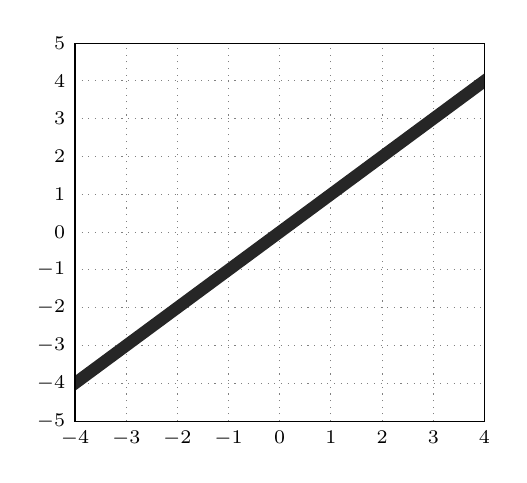
\begin{tikzpicture}[x=.65cm,y=.48cm,every node/.style={font=\scriptsize}]
\draw[step=1,dotted,gray] (-4,-5) grid (4,5);
\begin{scope}\clip (-4,-5) rectangle (4,5);
\fill[black!85] (-4,-4.2)--(4,3.8)--(4,4.2)--(-4,-3.8)--cycle;
\end{scope}
\draw (-4,-5) rectangle (4,5);
\foreach \x in {-4,-3,-2,-1,0,1,2,3,4}{\node[below] at (\x,-5) {$\x$};}
\foreach \y in {-5,-4,-3,-2,-1,0,1,2,3,4,5}{\node[left] at (-4,\y) {$\y$};}
\end{tikzpicture}\quad$\blacklozenge$
\end{center}

% Source: printed p. 160; PDF p. 169
\noindent\textit{Bài tập 4.3.3.11.}\keepwithnext

Nhắc lại rằng~(4.9) dùng các bảng để biểu diễn quan hệ; dùng thuật ngữ về bảng có thể hữu ích khi trả lời một số câu hỏi sau.
\begin{enumerate}[label=\alph*.]
\item Nếu $R\subseteq S\times S$ là một quan hệ hai ngôi, hãy tìm một cách tự nhiên để tạo từ nó một đồ thị $G_R$ có các đỉnh $S$.
\item Tập $A$ các mũi tên trong $G_R$ là gì?
\item Các hàm nguồn và đích $\mathrm{src},\mathrm{tgt}:A\to S$ trong $G_R$ là gì?
\item Xét bảy hàng số trong bảng bên trái của~(4.9), bỏ qua các dấu ba chấm. Vẽ đồ thị tương ứng.
\item Làm tương tự với bảng bên phải của~(4.9).\nobreak\hfill$\diamond$
\end{enumerate}

\noindent\textit{Lời giải 4.3.3.11.}\keepwithnext
\begin{enumerate}[label=\alph*.]
\item Ta có hai phép chiếu $\pi_1,\pi_2:S\times S\to S$ và một ánh xạ bao hàm $i:R\subseteq S\times S$. Do đó ta có một đồ thị
\[
\begin{tikzcd}[column sep=large]
R\arrow[r,shift left=.7ex,"\pi_1\circ i"]\arrow[r,shift right=.7ex,"\pi_2\circ i"']&S
\end{tikzcd}
\]
Ý tưởng là với mỗi hàng trong bảng, ta vẽ một mũi tên từ giá trị ở cột thứ nhất đến giá trị ở cột thứ hai.
\item Đó là $R$, có thể gọi là ``tập các hàng của bảng''.\ctfournote{Bản gốc, tr.~160, viết ``the number of rows in the table'' (số hàng của bảng). Ở đây đang hỏi một tập hợp, và $R$ là tập các cặp được ghi thành hàng; số hàng là lực lượng $|R|$, không phải tập $R$. Vì vậy, lời diễn giải được sửa thành ``tập các hàng''.}
\item Đó là $\pi_1\circ i$ và $\pi_2\circ i$, có thể gọi là ``cột thứ nhất và cột thứ hai của bảng''. Nói cách khác, $G_R:=(S,R,\pi_1\circ i,\pi_2\circ i)$.
\item Bảy mũi tên liền nét trong đồ thị sau tương ứng với bảy hàng được thể hiện trong bảng bên trái; ta thêm ba mũi tên nét đứt để hoàn thiện hình
% Source: printed p. 161; PDF p. 170
(chúng vẫn thỏa mãn quan hệ $\le$).
\begin{center}
\begin{tikzpicture}[>=Stealth,every node/.style={font=\small},vertex/.style={circle,fill,inner sep=1.2pt}]
\node at (1,3) {Một phần của $G_{m\le n}$};
\draw (-.8,-.8) rectangle (2.8,2.7);
\node[vertex,label=above right:{$0$}] (v0) at (0,2) {};
\node[vertex,label=above:{$1$}] (v1) at (2,2) {};
\node[vertex,label=below right:{$2$}] (v2) at (0,0) {};
\node[vertex,label=above right:{$3$}] (v3) at (2,0) {};
\draw[->] (v0)--(v1);\draw[->] (v0)--(v2);\draw[->] (v0)--(v3);\draw[->] (v1)--(v2);
\draw[->,dashed] (v1)--(v3);\draw[->,dashed] (v2)--(v3);
\draw[->] (v0) to[out=140,in=100,looseness=10] (v0);
\draw[->] (v1) to[out=80,in=30,looseness=10] (v1);
\draw[->] (v2) to[out=190,in=260,looseness=10] (v2);
\draw[->,dashed] (v3) to[out=-30,in=-90,looseness=10] (v3);
\end{tikzpicture}
\end{center}
\item Bảy hàng, bảy mũi tên:
\begin{samepage}
\begin{center}
\begin{tikzpicture}[>=Stealth,every node/.style={font=\small},vertex/.style={circle,fill,inner sep=1.2pt}]
\node at (1.6,1.3) {Một phần của $G_{|n-m|\le1}$};
\draw (-.65,-.65) rectangle (3.85,1);
\foreach \i in {0,1,2}{\node[vertex,label=below:{$\i$}] (v\i) at (1.6*\i,0) {};\draw[->] (v\i) to[out=130,in=50,looseness=10] (v\i);}
\draw[->] (v0) to[bend left=8] (v1);\draw[->] (v1) to[bend left=8] (v0);
\draw[->] (v1) to[bend left=8] (v2);\draw[->] (v2) to[bend left=8] (v1);
\end{tikzpicture}
\end{center}
\hfill$\blacklozenge$
\end{samepage}
\end{enumerate}

\noindent\textit{Bài tập 4.3.3.12.}\keepwithnext
\begin{enumerate}[label=\alph*.]
\item Nếu $(V,A,\mathrm{src},\mathrm{tgt})$ là một đồ thị, hãy tìm một cách tự nhiên để tạo từ nó một quan hệ hai ngôi $R\subseteq V\times V$.
\item Với đồ thị $G$ bên trái trong~(4.7), viết quan hệ hai ngôi tương ứng dưới dạng bảng.\nobreak\hfill$\diamond$
\end{enumerate}

\noindent\textit{Lời giải 4.3.3.12.}\keepwithnext
\begin{enumerate}[label=\alph*.]
\item Vì có các hàm $\mathrm{src},\mathrm{tgt}:A\to V$, tính chất phổ dụng của tích cho ta một hàm $\langle\mathrm{src},\mathrm{tgt}\rangle:A\to V\times V$. Đây chưa phải một quan hệ hai ngôi, vì nó có thể không đơn ánh. Vì vậy, cho $R\subseteq V\times V$ là ảnh của $\langle\mathrm{src},\mathrm{tgt}\rangle$; bây giờ ta đã có quan hệ hai ngôi mong muốn.
% Source: printed p. 162; PDF p. 171
\item
\[
\begin{array}{|r|r|}\hline1&2\\\hline1&4\\\hline2&3\\\hline5&6\\\hline\end{array}
\tag*{$\blacklozenge$}
\]
\end{enumerate}

\noindent\textit{Bài tập 4.3.3.13.}\keepwithnext
\begin{enumerate}[label=\alph*.]
\item Cho một quan hệ hai ngôi $R\subseteq S\times S$, bạn biết từ Bài tập~4.3.3.11 cách xây dựng một đồ thị từ nó, và từ Bài tập~4.3.3.12 cách tạo một quan hệ hai ngôi mới từ đồ thị ấy, hoàn thành một vòng đi rồi quay lại. Quan hệ thu được so với quan hệ ban đầu như thế nào?
\item Cho một đồ thị $G=(V,A,\mathrm{src},\mathrm{tgt})$, bạn biết từ Bài tập~4.3.3.12 cách tạo một quan hệ hai ngôi mới từ nó, và từ Bài tập~4.3.3.11 cách xây dựng một đồ thị mới từ quan hệ ấy, hoàn thành vòng đi rồi quay lại theo chiều ngược. Đồ thị thu được so với đồ thị ban đầu như thế nào?\nobreak\hfill$\diamond$
\end{enumerate}

\noindent\textit{Lời giải 4.3.3.13.}\keepwithnext
\begin{enumerate}[label=\alph*.]
\item Nó vẫn như cũ.
\item Nó khác đi. Đồ thị mới $G'$ không bao giờ có hai mũi tên cùng hướng. Nghĩa là trong đồ thị ban đầu $G$, ta có thể có hai mũi tên khác nhau $v_1\to v_2$, nhưng điều này không thể xảy ra trong đồ thị mới. Vì vậy đồ thị cũ và đồ thị mới có cùng số đỉnh, và có một mũi tên $v_1\to v_2$ trong $G$ khi và chỉ khi có một mũi tên $v_1\to v_2$ trong $G'$; nhưng nhiều mũi tên từ một đỉnh đến một đỉnh khác trong $G$ bị gộp thành một mũi tên duy nhất trong $G'$.\nobreak\hfill$\blacklozenge$
\end{enumerate}

\section{Thứ tự}

Người ta thường nghĩ một số tập hợp nhất định vốn có một thứ tự chính tắc. Chẳng hạn, ta có thể nghĩ rằng các số tự nhiên vốn có thứ tự trong đó $3<5$, hoặc các chữ cái trong bảng chữ cái vốn có thứ tự trong đó $b<e$. Nhưng thực ra, chúng ta đặt các thứ tự lên tập hợp, và chỉ là một số thứ tự được dùng phổ biến hơn. Chẳng hạn, ta có thể
% Sentence continues on printed p. 163.

% Source: printed p. 163; PDF p. 172
sắp thứ tự các chữ cái trong bảng chữ cái theo tần suất sử dụng; khi đó $e$ sẽ đứng trước $b$. Với những mục đích khác nhau, ta có thể đặt những thứ tự khác nhau trên cùng một tập hợp. Chẳng hạn, trong Ví dụ~4.4.3.2, ta cho một thứ tự khác trên các số tự nhiên, hữu ích trong lý thuyết số sơ cấp.

Trong khoa học, ta có thể sắp thứ tự tập các vật liệu theo hai cách khác nhau. Theo cách thứ nhất, ta xem vật liệu $A$ nhỏ hơn vật liệu $B$ nếu $A$ là một thành phần hay bộ phận của $B$; như vậy nước nhỏ hơn bê tông. Nhưng ta cũng có thể sắp thứ tự vật liệu dựa trên độ dẫn điện của chúng; khi đó bê tông nhỏ hơn nước. Mục này bàn về những loại thứ tự khác nhau.

\subsection{Định nghĩa tiền thứ tự, thứ tự bộ phận và thứ tự tuyến tính}

\noindent\textbf{Định nghĩa 4.4.1.1.} Cho $S$ là một tập hợp và $R\subseteq S\times S$ là một quan hệ hai ngôi trên $S$; nếu $(s,s')\in R$, ta viết $s\le s'$. Khi đó ta nói $R$ là một \emph{tiền thứ tự} nếu với mọi $s,s',s''\in S$, ta có
\begin{description}
\item[Tính phản xạ:] $s\le s$, và
\item[Tính bắc cầu:] nếu $s\le s'$ và $s'\le s''$ thì $s\le s''$.
\end{description}
Ta nói $R$ là một \emph{thứ tự bộ phận} nếu nó là một tiền thứ tự và thêm vào đó, với mọi $s,s'\in S$, ta có
\begin{description}
\item[Tính phản đối xứng:] Nếu $s\le s'$ và $s'\le s$ thì $s=s'$.
\end{description}
Ta nói $R$ là một \emph{thứ tự tuyến tính} nếu nó là một thứ tự bộ phận và thêm vào đó, với mọi $s,s'\in S$, ta có
\begin{description}
\item[Tính so sánh được:] Hoặc $s\le s'$ hoặc $s'\le s$.
\end{description}
Ta ký hiệu một tiền thứ tự (hoặc thứ tự bộ phận, hoặc thứ tự tuyến tính) như vậy là $(S,\le)$.

\noindent\textit{Bài tập 4.4.1.2.}\keepwithnext
\begin{enumerate}[label=\alph*.]
\item Quan hệ trong bảng bên trái của~(4.9) là một tiền thứ tự. Nó có phải một thứ tự tuyến tính không?
\item Chỉ ra rằng cả bảng ở giữa lẫn bảng bên phải trong~(4.9) đều thậm chí không phải tiền thứ tự.\nobreak\hfill$\diamond$
\end{enumerate}

\noindent\textit{Lời giải 4.4.1.2.}\keepwithnext
\begin{enumerate}[label=\alph*.]
\item Có.
% Source: printed p. 164; PDF p. 173
\item Nếu $\le$ biểu thị quan hệ ở giữa $n=5m$, ta không có tính phản xạ $(1\nleq1)$ lẫn tính bắc cầu ($25=5*5$ và $5=5*1$, nhưng $25\ne5*1$).\ctfournote{Bản gốc, tr.~164, in $25=5*1$ ở đẳng thức thứ nhất. Phản ví dụ cho tính bắc cầu phải dùng $1\le5$, $5\le25$ nhưng $1\nleq25$ theo quan hệ $n=5m$; vì vậy đẳng thức thứ nhất được sửa thành $25=5*5$.} Nếu $\le$ biểu thị quan hệ bên phải $|n-m|\le1$, ta có tính phản xạ nhưng không có tính bắc cầu.\nobreak\hfill$\blacklozenge$
\end{enumerate}

\noindent\textit{Ví dụ 4.4.1.3 (Thứ tự bộ phận nhưng không phải thứ tự tuyến tính).} Dưới đây là một olog cho các lá bài:
\stepcounter{equation}
\begin{equation}
\begin{tikzpicture}[>=Stealth,every node/.style={font=\footnotesize},concept/.style={draw,rectangle,align=center,inner sep=3pt,text width=1.65cm}]
\node[concept] (diamond) at (0,3.8) {một lá rô};
\node[concept] (heart) at (3,3.8) {một lá cơ};
\node[concept] (club) at (6,3.8) {một lá tép};
\node[concept] (spade) at (9,3.8) {một lá bích};
\node[concept] (red) at (1.5,2.55) {một lá bài đỏ};
\node[concept] (black) at (7.5,2.55) {một lá bài đen};
\node[concept] (card) at (4.5,1.15) {một lá bài};
\node[concept] (fourdiamond) at (0,1.15) {một lá 4 rô};
\node[concept] (blackqueen) at (9,1.15) {một lá Q đen};
\node[concept] (four) at (0,-.45) {một lá 4};
\node[concept] (numbered) at (3,-.45) {một lá bài số};
\node[concept] (face) at (6,-.45) {một lá bài hình};
\node[concept] (queen) at (9,-.45) {một lá Q};
\foreach \a/\b in {diamond/red,heart/red,club/black,spade/black,red/card,black/card,fourdiamond/diamond,fourdiamond/four,four/numbered,numbered/card,blackqueen/black,blackqueen/queen,queen/face,face/card}{\draw[->] (\a)--node[midway,above,sloped] {là}(\b);}
\end{tikzpicture}
\tag{4.10}
\end{equation}
Ta có thể đặt một quan hệ hai ngôi trên tập các hộp ở đây bằng cách nói $A\le B$ nếu có một đường đi $A\to B$. Ta thấy ngay đây là một tiền thứ tự, vì các đường đi có độ dài $0$ cho tính phản xạ, còn phép nối đường đi cho tính bắc cầu. Để thấy nó là một thứ tự bộ phận, ta chỉ cần nhận xét rằng không có vòng nào có độ dài dương.\ctfournote{Bản gốc, tr.~164, nói ``no loops of any length'' (không có vòng ở bất kỳ độ dài nào). Mọi đỉnh đều có đường đi tầm thường có độ dài $0$; để lập luận đúng, cần chỉ loại trừ các vòng có độ dài dương.} Nhưng thứ tự bộ phận này không phải thứ tự tuyến tính, vì không có đường đi (theo cả hai chiều), chẳng hạn, giữa $\ulcorner\text{một lá 4 rô}\urcorner$ và $\ulcorner\text{một lá Q đen}\urcorner$, nên nó vi phạm điều kiện so sánh được.

\noindent\textit{Nhận xét 4.4.1.4.} Chú ý rằng olog~(4.10) trong Ví dụ~4.4.1.3 là một olog tốt theo nghĩa: với bất kỳ tập bài nào (chẳng hạn chọn ngẫu nhiên 45 lá từ mỗi bộ trong bảy bộ bài rồi gom lại thành một chồng), ta có thể phân loại chúng theo olog ấy. Nói cách khác, mỗi hộp trong olog chỉ một tập con nào đó của chồng bài, và mỗi mũi tên chỉ một hàm giữa các tập này. Chẳng hạn, mũi tên $\ulcorner\text{một lá cơ}\urcorner\xrightarrow{\text{là}}\ulcorner\text{một lá bài đỏ}\urcorner$ là một hàm từ tập các lá cơ trong chồng bài đến tập các lá bài đỏ trong chồng bài.

\noindent\textit{Ví dụ 4.4.1.5 (Tiền thứ tự nhưng không phải thứ tự bộ phận).} Mọi quan hệ tương đương đều là một tiền thứ tự, nhưng chúng hiếm khi là thứ tự bộ phận. Chẳng hạn, nếu $S=\{1,2\}$ và đặt $R=S\times S$, thì đây là một quan hệ tương đương. Nó là tiền thứ tự nhưng không phải thứ tự bộ phận (vì $1\le2$ và $2\le1$, nhưng $1\ne2$, nên tính phản đối xứng không đúng).

% Source: printed p. 165; PDF p. 174
\noindent\textit{Ứng dụng 4.4.1.6.} Theo quan niệm cổ điển, ta xem thời gian là có thứ tự tuyến tính. Một mô hình là $(\mathbb{R},\le)$, thứ tự tuyến tính thông thường trên tập các số thực. Nhưng theo thuyết tương đối, thực ra không có một thứ tự duy nhất cho các sự kiện trong vũ trụ. Những người quan sát khác nhau quan sát đúng những thứ tự khác nhau trên tập các sự kiện.\hfill$\diamond\diamond$

\noindent\textit{Ví dụ 4.4.1.7 (Các thứ tự tuyến tính hữu hạn).} Cho $n\in\mathbb{N}$ là một số tự nhiên. Định nghĩa một thứ tự tuyến tính $[n]=(\{0,1,2,\ldots,n\},\le)$ theo cách tiêu chuẩn. Dưới dạng hình vẽ,
\[
[n]:=\begin{tikzcd}[column sep=large]
0\arrow[r,"\le"]&1\arrow[r,"\le"]&2\arrow[r,"\le"]&\cdots\arrow[r,"\le"]&n
\end{tikzcd}
\]
Mọi thứ tự tuyến tính hữu hạn khác rỗng, tức thứ tự tuyến tính trên một tập hữu hạn khác rỗng, đều có dạng trên.\ctfournote{Bản gốc, tr.~165, viết ``Every finite linear order'' mà không loại trừ tập rỗng. Các tập trong $[n]$ ở đây có $n+1$ phần tử với $n\in\mathbb{N}$, nên không bao gồm thứ tự duy nhất trên tập rỗng; điều kiện khác rỗng được bổ sung.} Nghĩa là mặc dù các nhãn có thể thay đổi, hình vẽ vẫn như nhau. Điều này có thể được làm chính xác khi cấu xạ giữa các thứ tự được định nghĩa (xem Định nghĩa~4.4.4.1).

\noindent\textit{Bài tập 4.4.1.8.}\keepwithnext

Cho $S=\{1,2,3\}$.
\begin{enumerate}[label=\alph*.]
\item Tìm một tiền thứ tự $R\subseteq S\times S$ sao cho tập $R$ nhỏ nhất có thể. Nó có phải một thứ tự bộ phận không? Có phải một thứ tự tuyến tính không?
\item Tìm một tiền thứ tự $R'\subseteq S\times S$ sao cho tập $R'$ lớn nhất có thể. Nó có phải một thứ tự bộ phận không? Có phải một thứ tự tuyến tính không?\nobreak\hfill$\diamond$
\end{enumerate}

\noindent\textit{Lời giải 4.4.1.8.}\keepwithnext

Viết $R$ và $R'$ thành các bảng:
\[
\begin{array}{|r|r|}\hline\multicolumn{2}{|c|}{R}\\\hline1&1\\\hline2&2\\\hline3&3\\\hline\end{array}
\qquad\qquad
\begin{array}{|r|r|}\hline\multicolumn{2}{|c|}{R'}\\\hline
1&1\\\hline1&2\\\hline1&3\\\hline2&1\\\hline2&2\\\hline2&3\\\hline3&1\\\hline3&2\\\hline3&3\\\hline
\end{array}
\]
% Source: printed p. 166; PDF p. 175
\begin{enumerate}[label=\alph*.]
\item $R$ là một thứ tự bộ phận nhưng không phải thứ tự tuyến tính, vì $1\nleq2$ và $2\nleq1$.
\item $R'$ không phải một thứ tự bộ phận, vì $1\le2$ và $2\le1$, nên không thể là thứ tự tuyến tính.\nobreak\hfill$\blacklozenge$
\end{enumerate}

\noindent\textit{Bài tập 4.4.1.9.}\keepwithnext
\begin{enumerate}[label=\alph*.]
\item Liệt kê mọi quan hệ tiền thứ tự có thể có trên tập $\{1,2\}$.
\item Với mọi $n\in\mathbb{N}$, có bao nhiêu thứ tự tuyến tính trên tập $\{1,2,3,\ldots,n\}$?
\item Công thức của bạn có đúng khi $n=0$ không?\nobreak\hfill$\diamond$
\end{enumerate}

\noindent\textit{Lời giải 4.4.1.9.}\keepwithnext
\begin{enumerate}[label=\alph*.]
\item
\[
\begin{array}{|r|r|}\hline\multicolumn{2}{|c|}{R_1}\\\hline1&1\\\hline2&2\\\hline\end{array}\qquad
\begin{array}{|r|r|}\hline\multicolumn{2}{|c|}{R_2}\\\hline1&1\\\hline1&2\\\hline2&2\\\hline\end{array}\qquad
\begin{array}{|r|r|}\hline\multicolumn{2}{|c|}{R_3}\\\hline1&1\\\hline2&1\\\hline2&2\\\hline\end{array}\qquad
\begin{array}{|r|r|}\hline\multicolumn{2}{|c|}{R_4}\\\hline1&1\\\hline1&2\\\hline2&1\\\hline2&2\\\hline\end{array}
\]
\item Giai thừa $n!=1*2*\cdots*n$.
\item Có, có một cách để sắp thứ tự tập rỗng, cụ thể là $\varnothing\subseteq\varnothing\times\varnothing$, và $0!=1$.\nobreak\hfill$\blacklozenge$
\end{enumerate}

\noindent\textit{Nhận xét 4.4.1.10.} Ta có thể vẽ mọi tiền thứ tự $(S,\le)$ thành một đồ thị có các đỉnh $S$ và một mũi tên $a\to b$ nếu $a\le b$. Đây chính là những đồ thị có hai tính chất sau với mọi đỉnh $a,b\in S$:
\begin{enumerate}
\item Có nhiều nhất một mũi tên $a\to b$.
\item Nếu có một đường đi từ $a$ đến $b$, thì có một mũi tên $a\to b$.
\end{enumerate}
Nếu $(S,\le)$ là một thứ tự bộ phận, thì đồ thị tương ứng còn có tính chất không có vòng đi qua các đỉnh khác nhau:
\begin{enumerate}[resume]
\item Nếu $n\in\mathbb{N}$ với $n\ge2$, thì mọi đường đi có độ dài $n$ bắt đầu tại $a$ và kết thúc tại $a$ chỉ đi qua đỉnh $a$.\ctfournote{Bản gốc, tr.~166, nói ``no paths of length $n$ that start at $a$ and end at $a$''. Điều đó không đúng, vì tính phản xạ đã cho một vòng $a\to a$, và lặp vòng này cho các đường đi kín ở mọi độ dài. Tính phản đối xứng chỉ loại trừ đường đi kín đi qua một đỉnh khác $a$: nếu đường đi đi qua $b$, ta có $a\le b$ và $b\le a$, nên $a=b$. Tính chất~3 được hiệu chỉnh theo nghĩa này.}
\end{enumerate}

% Source: printed p. 167; PDF p. 176
Nếu $(S,\le)$ là một thứ tự tuyến tính thì còn có thêm tính chất so sánh được:
\begin{enumerate}[resume]
\item Với mọi hai đỉnh $a,b$, có một mũi tên $a\to b$ hoặc một mũi tên $b\to a$.
\end{enumerate}
Cho một đồ thị $G$, ta có thể tạo một quan hệ hai ngôi $\le$ trên tập đỉnh $S$ như sau. Đặt $a\le b$ nếu có một đường đi từ $a$ đến $b$ trong $G$. Quan hệ này phản xạ và bắc cầu, nên là một tiền thứ tự. Nếu đồ thị thỏa mãn tính chất~3, thì tiền thứ tự sẽ là một thứ tự bộ phận; và nếu đồ thị còn thỏa mãn tính chất~4, thì thứ tự bộ phận sẽ là một thứ tự tuyến tính. Như vậy, đồ thị cho ta một cách tốt để hình dung các thứ tự.

\noindent\textit{Phương châm 4.4.1.11.}\keepwithnext
\begin{quote}\emph{Một đồ thị sinh ra một tiền thứ tự: $v\le w$ nếu có một đường đi $v\to w$.}\end{quote}

\noindent\textit{Bài tập 4.4.1.12.}\keepwithnext

Cho $G=(V,A,\mathrm{src},\mathrm{tgt})$ là đồ thị sau:
\begin{center}
\begin{tikzpicture}[>=Stealth,every node/.style={font=\small},vertex/.style={circle,fill,inner sep=1.2pt}]
\draw (-.5,-.5) rectangle (6.5,2.2);
\node[vertex,label=above:{$a$}] (a) at (0,1.5) {};
\node[vertex,label=above:{$b$}] (b) at (2,1.5) {};
\node[vertex,label=above:{$c$}] (c) at (4,1.5) {};
\node[vertex,label=above:{$d$}] (d) at (6,1.5) {};
\node[vertex,label=above:{$e$}] (e) at (0,0) {};
\node[vertex,label=above:{$f$}] (f) at (2,0) {};
\node[vertex,label=above:{$g$}] (g) at (4,0) {};
\draw[->] (a)--(b);\draw[->] (b) to[bend left=30] (c);\draw[->] (c) to[bend left=30] (b);
\draw[->] (c)--(d);\draw[->] (f)--(e);\draw[->] (f)--(g);\draw[->] (g)--(d);
\end{tikzpicture}
\end{center}
Trong tiền thứ tự tương ứng, những điều nào sau đây đúng?
\begin{enumerate}[label=\alph*.]
\item $a\le b$.
\item $a\le d$.
\item $c\le b$.
\item $b=c$.
\item $e\le f$.
\item $f\le d$.\nobreak\hfill$\diamond$
\end{enumerate}

\noindent\textit{Lời giải 4.4.1.12.}\keepwithnext
\begin{enumerate}[label=\alph*.]
\item Đúng.
% Source: printed p. 168; PDF p. 177
\item Đúng.
\item Đúng.
\item Sai (mặc dù điều này đúng trong thứ tự bộ phận tương ứng, mà ta chưa bàn đến).
\item Sai.
\item Đúng.\nobreak\hfill$\blacklozenge$
\end{enumerate}

\noindent\textit{Bài tập 4.4.1.13.}\keepwithnext
\begin{enumerate}[label=\alph*.]
\item Cho $S=\{1,2\}$. Tập $\mathbb{P}(S)$ các tập con của $S$ tạo thành một thứ tự bộ phận. Vẽ đồ thị tương ứng.
\item Lặp lại điều này cho $Q=\varnothing$, $R=\{1\}$ và $T=\{1,2,3\}$. Nghĩa là vẽ các thứ tự bộ phận trên $\mathbb{P}(Q)$, $\mathbb{P}(R)$ và $\mathbb{P}(T)$.
\item Bạn có thấy các khối lập phương $n$ chiều không?\nobreak\hfill$\diamond$
\end{enumerate}

\noindent\textit{Lời giải 4.4.1.13.}\keepwithnext
\begin{enumerate}[label=\alph*.]
\item
\begin{center}
\begin{tikzpicture}[>=Stealth,every node/.style={font=\small},vertex/.style={circle,fill,inner sep=1.2pt}]
\node at (1,3) {$\mathbb{P}(\{1,2\})$};\draw (-.95,-.85) rectangle (3.2,2.7);
\node[vertex,label=above:{$\varnothing$}] (a) at (0,2) {};
\node[vertex,label=above:{$\{1\}$}] (b) at (2,2) {};
\node[vertex,label=below left:{$\{2\}$}] (c) at (0,0) {};
\node[vertex,label=below right:{$\{1,2\}$}] (d) at (2,0) {};
\draw[->] (a)--(b);\draw[->] (a)--(c);\draw[->] (a)--(d);\draw[->] (b)--(d);\draw[->] (c)--(d);
\end{tikzpicture}
\end{center}
% Source: printed p. 169; PDF p. 178
\item
\begin{center}
\begin{tikzpicture}[>=Stealth,every node/.style={font=\small},vertex/.style={circle,fill,inner sep=1.2pt},scale=.88]
\node at (0,1.3) {$\mathbb{P}(\varnothing)$};\draw (-.45,-.45) rectangle (.45,.75);
\node[vertex,label=above:{$\varnothing$}] (q) at (0,0) {};
\node at (2.35,1.3) {$\mathbb{P}(\{1\})$};\draw (1.25,-.45) rectangle (3.8,.75);
\node[vertex,label=above:{$\varnothing$}] (r0) at (1.7,0) {};
\node[vertex,label=above:{$\{1\}$}] (r1) at (3.25,0) {};
\draw[->] (r0)--(r1);
\node at (7.2,3.85) {$\mathbb{P}(\{1,2,3\})$};\draw (4.1,-2.25) rectangle (10.95,3.35);
\node[vertex,label=above left:{$\varnothing$}] (t0) at (5,2.5) {};
\node[vertex,label=above right:{$\{1\}$}] (t1) at (7.8,2.5) {};
\node[vertex,label=left:{$\{3\}$}] (t3) at (6.3,1.2) {};
\node[vertex,label=right:{$\{1,3\}$}] (t13) at (9.1,1.2) {};
\node[vertex,label=below left:{$\{2\}$}] (t2) at (5,-.1) {};
\node[vertex,label=above right:{$\{1,2\}$}] (t12) at (7.8,-.1) {};
\node[vertex,label=below left:{$\{2,3\}$}] (t23) at (6.3,-1.4) {};
\node[vertex,label=below right:{$\{1,2,3\}$}] (t123) at (9.1,-1.4) {};
\foreach \a/\b in {t0/t1,t0/t2,t0/t3,t1/t12,t1/t13,t3/t13,t3/t23,t2/t12,t2/t23,t13/t123,t12/t123,t23/t123}{\draw[->] (\a)--(\b);}
\end{tikzpicture}
\end{center}
\item Có. Đồ thị gắn với $\mathbb{P}(\underline{n})$ trông như một khối lập phương $n$ chiều.\ctfournote{Các hình trong lời giải gốc giữ lại những mũi tên thể hiện hình lập phương và bỏ các vòng phản xạ; hình ba chiều còn bỏ một số mũi tên bắc cầu. Bản dịch giữ nguyên những mũi tên được vẽ. Để khôi phục đầy đủ quan hệ bao hàm, lấy tiền thứ tự sinh bởi các đường đi, như Phương châm~4.4.1.11.}\nobreak\hfill$\blacklozenge$
\end{enumerate}

\noindent\textbf{Định nghĩa 4.4.1.14.} Cho $(S,\le)$ là một tiền thứ tự. Một \emph{clique} là một tập con $S'\subseteq S$ sao cho với mỗi $a,b\in S'$, ta có $a\le b$.

\noindent\textit{Bài tập 4.4.1.15.}\keepwithnext

Đúng hay sai: Một thứ tự bộ phận là một tiền thứ tự không có clique? (Nếu sai, có một phát biểu gần với nó nhưng đúng không?)\hfill$\diamond$

\noindent\textit{Lời giải 4.4.1.15.}\keepwithnext

Sai. Mỗi phần tử luôn nằm trong clique chỉ gồm chính nó, nên nếu $X$ là một thứ tự bộ phận có ít nhất một phần tử, thì nó có một clique. Nhưng có một phát biểu gần với nó là đúng. Hãy định nghĩa một \emph{clique không tầm thường} là một clique gồm từ hai phần tử trở lên.

\noindent\textit{Phương châm.}
\begin{samepage}
\begin{quote}\emph{Một thứ tự bộ phận là một tiền thứ tự không có clique không tầm thường.}\end{quote}
\hfill$\blacklozenge$
\end{samepage}

Cũng như mọi quan hệ đều sinh ra một quan hệ tương đương (xem Mệnh đề~3.3.1.7), mọi quan hệ cũng sinh ra một tiền thứ tự.

\noindent\textit{Ví dụ 4.4.1.16.} Cho $X$ là một tập hợp và $R\subseteq X\times X$ là một quan hệ. Với các phần tử $x,y\in X$, ta nói có một \emph{$R$-đường đi} từ $x$ đến $y$ nếu tồn tại một số tự nhiên $n\in\mathbb{N}$ và các phần tử $x_0,x_1,\ldots,x_n\in X$ sao cho
% Source: printed p. 170; PDF p. 179
\begin{enumerate}
\item $x=x_0$;
\item $x_n=y$;
\item với mọi $i\in\mathbb{N}$, nếu $0\le i\le n-1$ thì $(x_i,x_{i+1})\in R$.
\end{enumerate}
Cho $\overline{R}$ biểu thị quan hệ trong đó $(x,y)\in\overline{R}$ nếu có một $R$-đường đi từ $x$ đến $y$. Ta gọi $\overline{R}$ là \emph{tiền thứ tự sinh bởi $R$}, và ghi nhận một số sự kiện về $\overline{R}$:
\begin{description}
\item[Tính bao hàm.] Nếu $(x,y)\in R$ thì $(x,y)\in\overline{R}$. Nghĩa là $R\subseteq\overline{R}$.
\item[Tính phản xạ.] Với mọi $x\in X$, ta có $(x,x)\in\overline{R}$.
\item[Tính bắc cầu.] Với mọi $x,y,z\in X$, nếu $(x,y)\in\overline{R}$ và $(y,z)\in\overline{R}$ thì $(x,z)\in\overline{R}$.
\end{description}
Hãy viết $x\le y$ nếu $(x,y)\in\overline{R}$. Để kiểm tra khẳng định về tính bao hàm, dùng $n=1$, để $x_0=x$ và $x_n=y$. Để kiểm tra tính phản xạ, dùng $n=0$, để $x=x_0=y$, và điều kiện~3 đúng một cách hiển nhiên vì không có chỉ số nào cần kiểm tra. Để kiểm tra tính bắc cầu, giả sử cho các $R$-đường đi $x=x_0\le x_1\le\cdots\le x_n=y$ và $y=y_0\le y_1\le\cdots\le y_p=z$; khi đó $x=x_0\le x_1\le\cdots\le x_n\le y_1\le\cdots\le y_p=z$ là một $R$-đường đi từ $x$ đến $z$.

Ta có thể biến bất kỳ quan hệ nào thành một tiền thứ tự theo một cách chính tắc. Dưới đây là một trường hợp cụ thể của ý tưởng ấy.

Cho $X=\{a,b,c,d\}$ và giả sử cho quan hệ $\{(a,b),(b,c),(b,d),(d,c),(c,c)\}$. Nó không phản xạ cũng không bắc cầu, nên không phải một tiền thứ tự. Để biến nó thành một tiền thứ tự, ta làm theo quy trình trên. Bắt đầu với các $R$-đường đi có độ dài $n=0$, ta đưa $\{(a,a),(b,b),(c,c),(d,d)\}$ vào $\overline{R}$. Các $R$-đường đi có độ dài $1$ thêm vào những phần tử ban đầu $\{(a,b),(b,c),(b,d),(d,c),(c,c)\}$. Sự lặp lại (chẳng hạn $(c,c)$) được phép, nhưng từ đây trong ví dụ này ta chỉ viết những phần tử mới. Các $R$-đường đi có độ dài $2$ thêm $\{(a,c),(a,d)\}$ vào $\overline{R}$. Ta có thể kiểm tra rằng các $R$-đường đi có độ dài $3$ trở lên không thêm gì mới vào $\overline{R}$, nên ta đã hoàn tất. Quan hệ
\[
\overline{R}=\{(a,a),(b,b),(c,c),(d,d),(a,b),(b,c),(b,d),(d,c),(a,c),(a,d)\}
\]
phản xạ và bắc cầu, nên là một tiền thứ tự.

\noindent\textit{Bài tập 4.4.1.17.}\keepwithnext

Cho $X=\{a,b,c,d,e,f\}$ và cho $R=\{(a,b),(b,c),(b,d),(d,e),(f,a)\}$.
\begin{enumerate}[label=\alph*.]
\item Tiền thứ tự $\overline{R}$ sinh bởi $R$ là gì?
\item Nó có phải một thứ tự bộ phận không?\nobreak\hfill$\diamond$
\end{enumerate}

% Source: printed p. 171; PDF p. 180
\noindent\textit{Lời giải 4.4.1.17.}\keepwithnext

Bắt đầu bằng cách vẽ đồ thị tương ứng, giúp ta hình dung.
\begin{center}
\begin{tikzpicture}[>=Stealth,every node/.style={font=\small},vertex/.style={circle,fill,inner sep=1.2pt}]
\draw (-.5,-.5) rectangle (6.5,2.2);
\node[vertex,label=above:{$f$}] (f) at (0,1.5) {};
\node[vertex,label=above:{$a$}] (a) at (2,1.5) {};
\node[vertex,label=above:{$b$}] (b) at (4,1.5) {};
\node[vertex,label=above:{$c$}] (c) at (6,1.5) {};
\node[vertex,label=below:{$d$}] (d) at (4,0) {};
\node[vertex,label=above:{$e$}] (e) at (6,0) {};
\draw[->] (f)--(a);\draw[->] (a)--(b);\draw[->] (b)--(c);\draw[->] (b)--(d);\draw[->] (d)--(e);
\end{tikzpicture}
\end{center}
\begin{enumerate}[label=\alph*.]
\item Nó chưa phải một tiền thứ tự ngay từ đầu, vì ta cần đưa vào mọi đường đi, có tất cả 19 đường đi. Bạn có thể thấy $R$ ban đầu chính là các đường đi có độ dài $1$, ở một đoạn phía dưới trong bảng:
\[
\begin{array}{|c|c|}\hline\multicolumn{2}{|c|}{\overline R}\\\hline
a&a\\\hline b&b\\\hline c&c\\\hline d&d\\\hline e&e\\\hline f&f\\\hline
a&b\\\hline b&c\\\hline b&d\\\hline d&e\\\hline f&a\\\hline
a&c\\\hline a&d\\\hline b&e\\\hline f&b\\\hline
a&e\\\hline f&c\\\hline f&d\\\hline f&e\\\hline
\end{array}
\]
\item Có. Không có clique không tầm thường nào.\nobreak\hfill$\blacklozenge$
\end{enumerate}

\noindent\textit{Bài tập 4.4.1.18.}\keepwithnext

Cho $X$ là tập những người, và cho $R\subseteq X\times X$ là quan hệ với $(x,y)\in R$ nếu $x$ là con của $y$. Mô tả tiền thứ tự sinh bởi $R$ bằng ngôn ngữ thông thường.\hfill$\diamond$

\noindent\textit{Lời giải 4.4.1.18.}\keepwithnext

Đó là tiền thứ tự hậu duệ: $x\le y$ nếu $x$ là hậu duệ của $y$. Nhưng hãy chú ý: trong tiền thứ tự này, mọi người đều được xem là hậu duệ của chính mình.\hfill$\blacklozenge$

\subsection{Giao và hợp}

Cho $X$ là một tập hợp bất kỳ. Nhắc lại từ Định nghĩa~3.4.4.9 rằng tập lũy thừa của $X$, ký hiệu $\mathbb{P}(X)$, là tập các tập con của $X$. Có một thứ tự tự nhiên trên $\mathbb{P}(X)$ cho bởi quan hệ tập con,
% Source: printed p. 172; PDF p. 181
như trong Bài tập~4.4.1.13. Cho hai phần tử $a,b\in\mathbb{P}(X)$, ta có thể xem chúng là các tập con của $X$ và lấy giao của chúng làm một phần tử của $\mathbb{P}(X)$, ký hiệu $a\cap b$. Ta cũng có thể xem chúng là các tập con của $X$ và lấy hợp của chúng làm một phần tử của $\mathbb{P}(X)$, ký hiệu $a\cup b$. Các phép giao và hợp được khái quát hóa trong định nghĩa sau.

\noindent\textbf{Định nghĩa 4.4.2.1.} Cho $(S,\le)$ là một tiền thứ tự, và cho $s,t\in S$ là các phần tử. Một \emph{giao} (meet) của $s$ và $t$ là một phần tử $w\in S$ thỏa mãn tính chất phổ dụng sau:
\begin{itemize}
\item $w\le s$ và $w\le t$,
\item với mọi $x\in S$, nếu $x\le s$ và $x\le t$ thì $x\le w$.
\end{itemize}
Nếu $w$ là một giao của $s$ và $t$, ta viết $w\cong s\wedge t$.

Một \emph{hợp} (join) của $s$ và $t$ là một phần tử $w\in S$ thỏa mãn tính chất phổ dụng sau:
\begin{itemize}
\item $s\le w$ và $t\le w$,
\item với mọi $x\in S$, nếu $s\le x$ và $t\le x$ thì $w\le x$.
\end{itemize}
Nếu $w$ là một hợp của $s$ và $t$, ta viết $w\cong s\vee t$.

Nghĩa là giao của $s$ và $t$ là phần tử lớn nhất nhỏ hơn cả hai, tức một \emph{cận dưới lớn nhất}; còn hợp của $s$ và $t$ là phần tử nhỏ nhất lớn hơn cả hai, tức một \emph{cận trên nhỏ nhất}. Chú ý rằng giao của $s$ và $t$ có thể chính là $s$ hoặc $t$.

Có thể $s$ và $t$ có nhiều hơn một giao (hoặc nhiều hơn một hợp). Tuy nhiên, theo tính chất phổ dụng, bất kỳ hai giao nào của $s$ và $t$ đều phải nằm trong cùng một clique (và với hợp cũng vậy).

\noindent\textit{Bài tập 4.4.2.2.}\keepwithnext

Xét thứ tự bộ phận trong Ví dụ~4.4.1.3.
\begin{enumerate}[label=\alph*.]
\item Hợp của $\ulcorner\text{một lá rô}\urcorner$ và $\ulcorner\text{một lá cơ}\urcorner$ là gì?
\item Giao của $\ulcorner\text{một lá bài đen}\urcorner$ và $\ulcorner\text{một lá Q}\urcorner$ là gì?
\item Giao của $\ulcorner\text{một lá rô}\urcorner$ và $\ulcorner\text{một lá bài}\urcorner$ là gì?\nobreak\hfill$\diamond$
\end{enumerate}

\noindent\textit{Lời giải 4.4.2.2.}\keepwithnext
\begin{enumerate}[label=\alph*.]
\item $\ulcorner\text{một lá rô}\urcorner\vee\ulcorner\text{một lá cơ}\urcorner=\ulcorner\text{một lá bài đỏ}\urcorner$.
\item $\ulcorner\text{một lá bài đen}\urcorner\wedge\ulcorner\text{một lá Q}\urcorner=\ulcorner\text{một lá Q đen}\urcorner$.
% Source: printed p. 173; PDF p. 182
\item $\ulcorner\text{một lá rô}\urcorner\wedge\ulcorner\text{một lá bài}\urcorner=\ulcorner\text{một lá rô}\urcorner$.\nobreak\hfill$\blacklozenge$
\end{enumerate}

Không phải bất kỳ hai phần tử nào của một tiền thứ tự cũng cần có giao, và chúng cũng không nhất thiết có hợp.

\noindent\textit{Bài tập 4.4.2.3.}\keepwithnext
\begin{enumerate}[label=\alph*.]
\item Nếu có thể, tìm hai phần tử trong thứ tự bộ phận của Ví dụ~4.4.1.3 không có giao.\footnote{Dùng tiền thứ tự được thể hiện trong hình, không dùng bất kỳ phép hoàn thiện nào của những gì được viết ở đó.}
\item Nếu có thể, tìm hai phần tử không có hợp (trong tiền thứ tự ấy).\nobreak\hfill$\diamond$
\end{enumerate}

\noindent\textit{Lời giải 4.4.2.3.}\keepwithnext
\begin{enumerate}[label=\alph*.]
\item Không có giao của $\ulcorner\text{một lá cơ}\urcorner$ và $\ulcorner\text{một lá tép}\urcorner$; không lá bài nào đồng thời thuộc cả hai loại.
\item Mọi hai phần tử ở đây đều có hợp. Nhưng chú ý rằng một số hợp này là ``sai'', vì olog chưa đầy đủ. Chẳng hạn, ta có $\ulcorner\text{một lá 4}\urcorner\vee\ulcorner\text{một lá Q}\urcorner=\ulcorner\text{một lá bài}\urcorner$, trong khi câu trả lời đúng phải là $\ulcorner\text{một lá bài là lá 4 hoặc lá Q}\urcorner$.\nobreak\hfill$\blacklozenge$
\end{enumerate}

\noindent\textit{Bài tập 4.4.2.4.}\keepwithnext

Như đã nói, tập lũy thừa $S:=\mathbb{P}(X)$ của bất kỳ tập $X$ nào tự nhiên có cấu trúc thứ tự bộ phận. Các phần tử $s\in S$ tương ứng với các tập con $s\subseteq X$, và ta đặt $s\le t$ khi và chỉ khi $s\subseteq t$ như các tập con của $X$. Giao của hai phần tử là giao của chúng như các tập con của $X$, $s\wedge t=s\cap t$, còn hợp của hai phần tử là hợp của chúng như các tập con của $X$, $s\vee t=s\cup t$.
\begin{enumerate}[label=\alph*.]
\item Có thể trang bị một cấu trúc monoid trên tập $S$ mà công thức nhân được cho bởi các giao không? Nếu có, phần tử đơn vị là gì?
\item Có thể trang bị một cấu trúc monoid trên tập $S$ mà công thức nhân được cho bởi các hợp không? Nếu có, phần tử đơn vị là gì?\nobreak\hfill$\diamond$
\end{enumerate}

% Source: printed p. 174; PDF p. 183
\noindent\textit{Lời giải 4.4.2.4.}\keepwithnext
\begin{enumerate}[label=\alph*.]
\item Có. Phần tử đơn vị là tập con $X\subseteq X$, vì với mọi $s\in\mathbb{P}(X)$, ta có $X\wedge s=X\cap s=s$. Vì vậy monoid là $(\mathbb{P}(X),X,\cap)$.
\item Có. Phần tử đơn vị là tập con $\varnothing\subseteq X$, vì với mọi $s\in\mathbb{P}(X)$, ta có $\varnothing\vee s=\varnothing\cup s=s$. Vì vậy monoid là $(\mathbb{P}(X),\varnothing,\cup)$.\nobreak\hfill$\blacklozenge$
\end{enumerate}

\noindent\textit{Ví dụ 4.4.2.5 (Cây).} Một \emph{cây}, tức một hệ thống các nút và nhánh, tất cả đều phát ra từ một nút duy nhất gọi là \emph{gốc}, là một thứ tự bộ phận nhưng nói chung không phải thứ tự tuyến tính. Một cây $(T,\le)$ có thể được định hướng về gốc (khi đó gốc là phần tử lớn nhất của thứ tự bộ phận) hoặc ra xa gốc (khi đó gốc là phần tử nhỏ nhất); ta chỉ xét trường hợp thứ nhất.

Một cây được vẽ dưới dạng đồ thị trong~(4.11). Gốc được gắn nhãn $e$.
\stepcounter{equation}
\begin{equation}
\begin{tikzpicture}[>=Stealth,every node/.style={font=\small},vertex/.style={circle,fill,inner sep=1.2pt}]
\node[vertex,label=above:{$e$}] (e) at (0,0) {};
\node[vertex,label=above:{$b$}] (b) at (1.5,1.1) {};
\node[vertex,label=above:{$c$}] (c) at (3,1.1) {};
\node[vertex,label=above:{$a$}] (a) at (4.5,2.2) {};
\node[vertex,label=above:{$d$}] (d) at (4.5,1.1) {};
\node[vertex,label=above:{$f$}] (f) at (4.5,0) {};
\node[vertex,label=above:{$g$}] (g) at (1.5,-1.1) {};
\node[vertex,label=above:{$h$}] (h) at (3,-1.1) {};
\node[vertex,label=above:{$i$}] (i) at (3,-2.2) {};
\foreach \x/\y in {a/c,d/c,f/c,c/b,b/e,g/e,h/g,i/g}{\draw[->] (\x)--(\y);}
\end{tikzpicture}
\tag{4.11}
\end{equation}
Trong một cây, mọi cặp phần tử $s,t\in T$ đều có một hợp $s\vee t$ (tổ tiên chung gần nhất của chúng). Mặt khác, nếu $s$ và $t$ có một giao $c=s\wedge t$, thì hoặc $c=s$ hoặc $c=t$.\ctfournote{Bản gốc, tr.~174, viết ``a join $s\wedge t$'' ở câu thứ nhất, và ``have a join $c=s\vee t$'' ở câu thứ hai. Với định hướng về gốc, tổ tiên chung gần nhất là hợp, ký hiệu $s\vee t$; còn giao chỉ tồn tại khi hai nút so sánh được và bằng một trong hai nút. Hai ký hiệu và từ ``join'' trong câu thứ hai được sửa tương ứng. Các lời giải~4.4.2.6 xác nhận cách dùng này.}

\noindent\textit{Bài tập 4.4.2.6.}\keepwithnext

Xét cây được vẽ trong~(4.11).
\begin{enumerate}[label=\alph*.]
\item Hợp $i\vee h$ là gì?
\item Hợp $h\vee b$ là gì?
\item Giao $b\wedge a$ là gì?
\item Giao $b\wedge g$ là gì?\nobreak\hfill$\diamond$
\end{enumerate}

% Source: printed p. 175; PDF p. 184
\noindent\textit{Lời giải 4.4.2.6.}\keepwithnext
\begin{enumerate}[label=\alph*.]
\item $i\vee h=g$.
\item $h\vee b=e$.
\item $b\wedge a=a$.
\item $b\wedge g$ không tồn tại.\nobreak\hfill$\blacklozenge$
\end{enumerate}

\subsection{Thứ tự đối}

\noindent\textbf{Định nghĩa 4.4.3.1.} Cho $\mathcal{S}:=(S,\le)$ là một tiền thứ tự. \emph{Tiền thứ tự đối}, ký hiệu $\mathcal{S}^{\mathrm{op}}$, là tiền thứ tự $(S,\le^{\mathrm{op}})$ có cùng tập phần tử nhưng $s\le^{\mathrm{op}}s'$ khi và chỉ khi $s'\le s$.

\noindent\textit{Ví dụ 4.4.3.2.} Xét tiền thứ tự $\mathcal{N}:=(\mathbb{N},\text{là ước của})$, trong đó $a$ là ước của $b$ nếu ``$b$ chia cho $a$ được số nguyên'', tức tồn tại $n\in\mathbb{N}$ sao cho $a*n=b$. Vì vậy $5$ là ước của $35$, v.v. Khi đó $\mathcal{N}^{\mathrm{op}}$ là tập các số tự nhiên nhưng $m\le n$ khi và chỉ khi $m$ là một bội của $n$. Vì vậy $6\le2$ và $6\le3$, nhưng $6\nleq4$.

\noindent\textit{Bài tập 4.4.3.3.}\keepwithnext

Giả sử $\mathcal{S}:=(S,\le)$ là một tiền thứ tự.
\begin{enumerate}[label=\alph*.]
\item Nếu $\mathcal{S}$ là một thứ tự bộ phận, thì $\mathcal{S}^{\mathrm{op}}$ cũng là thứ tự bộ phận không?
\item Nếu $\mathcal{S}$ là một thứ tự tuyến tính, thì $\mathcal{S}^{\mathrm{op}}$ là thứ tự tuyến tính không?\nobreak\hfill$\diamond$
\end{enumerate}

\noindent\textit{Lời giải 4.4.3.3.}\keepwithnext
\begin{enumerate}[label=\alph*.]
\item Có. Nếu $\mathcal{S}$ không có clique không tầm thường, thì $\mathcal{S}^{\mathrm{op}}$ cũng không có.
\item Có. Nếu mọi hai phần tử của $\mathcal{S}$ đều so sánh được, thì mọi hai phần tử của $\mathcal{S}^{\mathrm{op}}$ cũng vậy.\nobreak\hfill$\blacklozenge$
\end{enumerate}

\noindent\textit{Bài tập 4.4.3.4.}\keepwithnext

Giả sử $\mathcal{S}:=(S,\le)$ là một tiền thứ tự, và $s_1,s_2\in S$ có hợp $s_1\vee s_2=t$ trong $\mathcal{S}$. Tiền thứ tự $\mathcal{S}^{\mathrm{op}}$ có cùng các phần tử như $\mathcal{S}$. $t$ có phải hợp của $s_1$ và $s_2$ trong $\mathcal{S}^{\mathrm{op}}$, hay là giao của chúng, hay không nhất thiết là giao cũng không nhất thiết là hợp của chúng?\hfill$\diamond$

% Source: printed p. 176; PDF p. 185
\noindent\textit{Lời giải 4.4.3.4.}\keepwithnext

Đó là giao của chúng.\hfill$\blacklozenge$

\subsection{Cấu xạ giữa các thứ tự}

Một thứ tự $(S,\le)$, dù là tiền thứ tự, thứ tự bộ phận hay thứ tự tuyến tính, gồm một tập hợp và một quan hệ hai ngôi. Để có thể so sánh hai thứ tự, các tập hợp và các quan hệ của chúng phải có thể được so sánh theo cách thích hợp.

\noindent\textbf{Định nghĩa 4.4.4.1.} Cho $\mathcal{S}:=(S,\le)$ và $\mathcal{S}':=(S',\le')$ là các tiền thứ tự (tương ứng, thứ tự bộ phận hoặc thứ tự tuyến tính). Một \emph{cấu xạ giữa các tiền thứ tự} (tương ứng, thứ tự bộ phận hoặc thứ tự tuyến tính) $f$ từ $\mathcal{S}$ đến $\mathcal{S}'$, ký hiệu $f:\mathcal{S}\to\mathcal{S}'$, là một hàm $f:S\to S'$ sao cho với mọi cặp phần tử $s_1,s_2\in S$, nếu $s_1\le s_2$ thì $f(s_1)\le'f(s_2)$.

\noindent\textit{Ví dụ 4.4.4.2.} Cho $X$ và $Y$ là các tập hợp, và cho $f:X\to Y$ là một hàm. Khi đó, với mọi tập con $X'\subseteq X$, ảnh $f(X')\subseteq Y$ của nó là một tập con (xem Bài tập~2.1.2.8). Vì vậy ta có một hàm $F:\mathbb{P}(X)\to\mathbb{P}(Y)$ được cho bằng phép lấy ảnh. Đây là một cấu xạ giữa các thứ tự bộ phận $(\mathbb{P}(X),\subseteq)\to(\mathbb{P}(Y),\subseteq)$. Thật vậy, nếu $a\subseteq b$ trong $\mathbb{P}(X)$, thì $f(a)\subseteq f(b)$ trong $\mathbb{P}(Y)$.

\noindent\textit{Ứng dụng 4.4.4.3.} Người ta thường nói rằng một nhóm chỉ mạnh bằng thành viên yếu nhất của nó. Điều này có đúng với vật liệu không? Giả thuyết rằng một vật liệu chỉ mạnh bằng thành phần yếu nhất của nó có thể được hiểu như sau.

Nhắc lại từ đầu Mục~4.4 (trang~162 của nguyên bản) rằng ta có thể đặt vài thứ tự khác nhau trên tập $M$ các vật liệu. Một ví dụ là thứ tự theo thành phần ($m\le_Cm'$ nếu $m$ là một nguyên liệu hay thành phần của $m'$). Một thứ tự khác được cho bởi độ bền: $m\le_Sm'$ nếu $m'$ bền hơn $m$ (trong một bối cảnh cố định).

Có đúng là nếu vật liệu $m$ là thành phần của vật liệu $m'$, thì độ bền của $m'$ nhỏ hơn hoặc bằng độ bền của $m$ không? Về mặt toán học, câu hỏi sẽ là: Có một cấu xạ tiền thứ tự $(M,\le_C)\to(M,\le_S)^{\mathrm{op}}$ không?\ctfournote{Để cấu xạ này mã hóa đúng giả thuyết vừa phát biểu, hàm nền cần là hàm đồng nhất trên $M$. Bản gốc chỉ hỏi sự tồn tại của một cấu xạ mà không chỉ rõ điều này; một hàm khác, chẳng hạn hàm hằng, có thể bảo toàn thứ tự mà không diễn đạt quan hệ về độ bền của cùng các vật liệu.}\nobreak\hfill$\diamond\diamond$

\noindent\textit{Bài tập 4.4.4.4.}\keepwithnext

Cho $X$ và $Y$ là các tập hợp, và cho $f:X\to Y$ là một hàm. Khi đó, với mọi tập con $Y'\subseteq Y$, nghịch ảnh $f^{-1}(Y')\subseteq X$ của nó là một tập con (xem Định nghĩa~3.2.1.12). Vì vậy ta có một hàm $F:\mathbb{P}(Y)\to\mathbb{P}(X)$ được cho bằng phép lấy nghịch ảnh. Nó có phải một cấu xạ giữa các thứ tự bộ phận không?\hfill$\diamond$

\noindent\textit{Lời giải 4.4.4.4.}\keepwithnext

Trước hết hãy đặt phần bàn luận trên một cơ sở cụ thể bằng một olog
\begin{center}
\begin{tikzpicture}[>=Stealth,every node/.style={font=\small}]
\node[draw,rectangle,label=above:{$X$}] (person) at (0,0) {một người};
\node[draw,rectangle,label=above:{$Y$}] (country) at (5,0) {một quốc gia};
\draw[->] (person)--node[above,font=\footnotesize] {sống ở}(country);
\end{tikzpicture}
\end{center}

% Source: printed p. 177; PDF p. 186
Bây giờ, cho bất kỳ tập các quốc gia $Y'\subseteq Y$, ta có thể xét tập $f^{-1}(Y')$ những người sống ở (một trong) các quốc gia đó: đây là nghịch ảnh. Câu hỏi này hỏi rằng nếu Mary chọn một tập các quốc gia $M\subseteq Y$ và John chọn tất cả những quốc gia ấy cùng một vài quốc gia nữa, $M\subseteq J$, thì tập những người sống ở các quốc gia do John chọn có chứa tập những người sống ở các quốc gia do Mary chọn không, $f^{-1}(M)\subseteq f^{-1}(J)$? Rõ ràng là có. Vì vậy $F=f^{-1}(-):\mathbb{P}(Y)\to\mathbb{P}(X)$ là một cấu xạ giữa các thứ tự bộ phận.\hfill$\blacklozenge$

\noindent\textit{Ví dụ 4.4.4.5.} Cho $S$ là một tập hợp. Cấu trúc tiền thứ tự nhỏ nhất có thể đặt trên $S$ là nói $a\le b$ khi và chỉ khi $a=b$. Quan hệ này đúng là phản xạ và bắc cầu, và được gọi là \emph{tiền thứ tự rời rạc} trên $S$.

Cấu trúc tiền thứ tự lớn nhất có thể đặt trên $S$ là nói $a\le b$ với mọi $a,b\in S$. Quan hệ này cũng phản xạ và bắc cầu, và được gọi là \emph{tiền thứ tự thô (indiscrete)} trên $S$.

\noindent\textit{Bài tập 4.4.4.6.}\keepwithnext

Cho $S$ là một tập hợp, và cho $(T,\le_T)$ là một tiền thứ tự. Cho $\le_D$ là tiền thứ tự rời rạc trên $S$.
\begin{enumerate}[label=\alph*.]
\item Một cấu xạ tiền thứ tự $(S,\le_D)\to(T,\le_T)$ là một hàm $S\to T$ thỏa mãn một số tính chất (xem Định nghĩa~4.4.4.1). Những hàm $S\to T$ nào xuất hiện theo cách này?
\item Cho một cấu xạ tiền thứ tự $(T,\le_T)\to(S,\le_D)$, ta được một hàm $T\to S$. Xét theo $\le_T$, những hàm $T\to S$ nào xuất hiện theo cách này?\nobreak\hfill$\diamond$
\end{enumerate}

\noindent\textit{Lời giải 4.4.4.6.}\keepwithnext
\begin{enumerate}[label=\alph*.]
\item Tất cả. Mọi hàm $S\to T$ đều tôn trọng tiền thứ tự rời rạc.
\item Ta được đúng những hàm $f:T\to S$ có tính chất sau với mọi $t_1,t_2\in T$: nếu $t_1\le_Tt_2$ thì $f(t_1)=f(t_2)$.\nobreak\hfill$\blacklozenge$
\end{enumerate}

\noindent\textit{Bài tập 4.4.4.7.}\keepwithnext

Cho $S$ là một tập hợp, và cho $(T,\le_T)$ là một tiền thứ tự. Cho $\le_I$ là tiền thứ tự thô trên $S$, như trong Ví dụ~4.4.4.5.
\begin{enumerate}[label=\alph*.]
\item Cho một cấu xạ tiền thứ tự $(S,\le_I)\to(T,\le_T)$, ta được một hàm $S\to T$. Xét theo $\le_T$, những hàm $S\to T$ nào xuất hiện theo cách này?
\item Cho một cấu xạ tiền thứ tự $(T,\le_T)\to(S,\le_I)$, ta được một hàm $T\to S$. Xét theo $\le_T$, những hàm $T\to S$ nào xuất hiện theo cách này?\hfill$\diamond$
\end{enumerate}

% Source: printed p. 178; PDF p. 187
\noindent\textit{Lời giải 4.4.4.7.}\keepwithnext
\begin{enumerate}[label=\alph*.]
\item Ta được đúng những hàm $f:S\to T$ có tính chất sau: tồn tại một clique $T'\subseteq T$ sao cho $f(S)\subseteq T'$.
\item Tất cả.\nobreak\hfill$\blacklozenge$
\end{enumerate}

\subsection{Những ứng dụng khác}
\subsubsection*{4.4.5.1\quad Phân loại sinh học}

Phân loại sinh học là một phương pháp chia tập các sinh vật thành những lớp khác nhau, gọi là các taxon. Thực ra, một hệ thống phân loại như vậy, chẳng hạn một cây phát sinh chủng loại, có thể được hiểu như một thứ tự bộ phận $C$ trên tập các taxon. Việc gán bậc điển hình cho những taxon này, gồm giới, ngành, v.v., có thể được hiểu như một cấu xạ thứ tự $f:C\to[n]$ với một $n\in\mathbb{N}$ nào đó.

Chẳng hạn, ta có thể có một cây (xem Ví dụ~4.4.2.5) trông như thế này:
\begin{center}
\begin{tikzpicture}[>=Stealth,every node/.style={font=\footnotesize},vertex/.style={circle,fill,inner sep=1.2pt}]
\node[vertex,label=left:{Sự sống}] (life) at (0,0) {};
\node[vertex,label=above:{Archaea}] (archaea) at (2,2) {};
\node[vertex,label=above:{Bacteria}] (bacteria) at (2,0) {};
\node[vertex,label=below:{Eukaryota}] (eukaryota) at (2,-2) {};
\node[vertex,label=above:{Pyrodicticum}] (pyro) at (5,2) {};
\node[vertex,label=above:{Spirochetes}] (spiro) at (5,1) {};
\node[vertex,label=above:{Aquifex}] (aquifex) at (5,0) {};
\node[vertex,label=above:{Nấm}] (fungi) at (5,-1) {};
\node[vertex,label=above:{Động vật}] (animals) at (5,-2) {};
\node (dots) at (7,-2) {$\cdots$};
\node[vertex,label=above:{HomoSapien}] (human) at (9.5,-2) {};
\foreach \a/\b in {archaea/life,bacteria/life,eukaryota/life,pyro/archaea,spiro/bacteria,aquifex/bacteria,fungi/eukaryota,animals/eukaryota,human/dots,dots/animals}{\draw[->] (\a)--(\b);}
\end{tikzpicture}
\end{center}
Ta cũng có một thứ tự tuyến tính trông như sau:
\begin{center}
\begin{tikzpicture}[>=Stealth,every node/.style={font=\footnotesize},vertex/.style={circle,fill,inner sep=1.2pt}]
\node[vertex,label=above:{Sự sống}] (life) at (0,0) {};
\node[vertex,label=above:{Vực}] (domain) at (1.8,0) {};
\node[vertex,label=above:{Giới}] (kingdom) at (3.6,0) {};
\node[vertex,label=above:{Ngành}] (phylum) at (5.4,0) {};
\node (dots) at (7.2,0) {$\cdots$};
\node[vertex,label=above:{Chi}] (genus) at (9,0) {};
\node[vertex,label=above:{Loài}] (species) at (10.8,0) {};
\foreach \a/\b in {species/genus,genus/dots,dots/phylum,phylum/kingdom,kingdom/domain,domain/life}{\draw[->] (\a)--(\b);}
\end{tikzpicture}
\end{center}
và hệ thống gán bậc đặt Eukaryota ở bậc Vực, Homo Sapien ở bậc Loài, là một hàm bảo toàn thứ tự từ các chấm ở hình trên đến các chấm ở hình dưới; nghĩa là đó là một cấu xạ tiền thứ tự.

% Source: printed p. 179; PDF p. 188
\noindent\textbf{Bài tập 4.4.5.2.}\keepwithnext
Vì cây phát sinh chủng loại là một cây nên nó có mọi hợp.
\begin{enumerate}[label=\alph*.]
\item Xác định hợp của chó và người.
\item Nếu ta không yêu cầu thứ tự bộ phận phát sinh chủng loại phải là một cây, thì việc hai taxon (các nút trong thứ tự bộ phận phát sinh chủng loại), chẳng hạn $a$ và $b$, có giao $c$ với $c\ne a$ và $c\ne b$ có ý nghĩa gì?\nobreak\hfill$\diamond$
\end{enumerate}

\noindent\textbf{Lời giải 4.4.5.2.}\keepwithnext
\begin{enumerate}[label=\alph*.]
\item Chó và người có hợp là lớp ``động vật có vú''.
\item Các điều kiện $a\wedge b\ne a$ và $a\wedge b\ne b$ có nghĩa là không có $a\le b$ cũng không có $b\le a$. Vì vậy, tình huống lạ này có nghĩa là taxon $c$ được phân loại như một taxon con của cả taxon $a$ lẫn taxon $b$, và là taxon con lớn nhất như vậy.\nobreak\hfill$\blacklozenge$
\end{enumerate}

\noindent\textbf{Bài tập 4.4.5.3.}\keepwithnext
\begin{enumerate}[label=\alph*.]
\item Trong lĩnh vực khoa học mà bạn yêu thích, có hệ thống phân loại thú vị nào thực sự là một thứ tự không?
\item Chọn một hệ thống như vậy; giao có ý nghĩa gì trong bối cảnh đó?\nobreak\hfill$\diamond$
\end{enumerate}

\noindent\textbf{Lời giải 4.4.5.3.}\keepwithnext
\begin{enumerate}[label=\alph*.]
\item Trong địa lý, có lẽ ta có thể phân loại các vùng chính trị theo việc chúng là các hiệp hội khu dân cư, thành phố/quận, bang/tỉnh, quốc gia hay thế giới.
\item Hợp của hai vùng chính trị sẽ là vùng nhỏ nhất chứa cả hai; chẳng hạn $\text{Chicago}\vee\text{North Carolina}=\text{Hoa Kỳ}$.\ctfournote{Nguyên bản hỏi về ``meets'' trong Bài tập~4.4.5.3(b), nhưng lời giải lại nói ``The join of two political regions''. Bản dịch giữ nguyên sự khác biệt giữa câu hỏi về giao và câu trả lời về hợp.}\nobreak\hfill$\blacklozenge$
\end{enumerate}

% Source: printed p. 180; PDF p. 189
\subsubsection*{4.4.5.4\quad Bảo mật}

Việc bảo mật, chẳng hạn bảo mật thông tin nhạy cảm, dựa trên hai yếu tố: mức cho phép tiếp cận thông tin mật và nhu cầu được biết. Mức cho phép có thể gồm các cấp như mật, tối mật, tuyệt mật. Nhưng có lẽ ta còn có thể thêm ``chỉ Tổng thống được đọc'' và một số cấp khác, chẳng hạn ``bất kỳ ai''.

\noindent\textbf{Bài tập 4.4.5.5.}\keepwithnext
Bạn thấy mức cho phép tiếp cận thông tin mật có vẻ là một tiền thứ tự, một thứ tự bộ phận hay một thứ tự tuyến tính?\nobreak\hfill$\diamond$

\noindent\textbf{Lời giải 4.4.5.5.}\keepwithnext
Có vẻ đó là một thứ tự tuyến tính.\nobreak\hfill$\blacklozenge$

``Nhu cầu được biết'' là một cách phân loại con người khác. Đối với mỗi mẩu thông tin, ta không nhất thiết muốn mọi người biết nó, ngay cả mọi người có mức cho phép đã chỉ định. Thông tin chỉ được phổ biến cho những người cần biết.

\noindent\textbf{Bài tập 4.4.5.6.}\keepwithnext
Cho $P$ là tập tất cả mọi người, và cho $\mathcal I$ là tập tất cả các mẩu thông tin mà chính phủ biết. Với mỗi tập con $I\subseteq\mathcal I$, cho $K(I)\subseteq P$ là tập những người cần biết mọi mẩu thông tin trong $I$. Cho $S=\{K(I)\mid I\subseteq\mathcal I\}$ là tập tất cả các nhóm ``cần được biết'', với quan hệ tập con được ký hiệu là $\le$.
\begin{enumerate}[label=\alph*.]
\item $(S,\le)$ có phải là một tiền thứ tự không? Nếu không, hãy tìm một tiền thứ tự gần với nó.
\item Nếu $I_1\subseteq I_2$, ta luôn có $K(I_1)\le K(I_2)$, hay $K(I_2)\le K(I_1)$, hay có thể không có cả hai?
\item Tiền thứ tự $(S,\le)$ có mọi giao không?
\item Tiền thứ tự $(S,\le)$ có mọi hợp không?\nobreak\hfill$\diamond$
\end{enumerate}

\noindent\textbf{Lời giải 4.4.5.6.}\keepwithnext
\begin{enumerate}[label=\alph*.]
\item Có, $(S,\le)$ là một tiền thứ tự.
\item Nếu Alice cần biết mọi mẩu thông tin trong $I_1$, và $I_1\subseteq I_2$, điều này không có nghĩa là cô ấy cần biết mọi thứ trong $I_2$; chiều ngược lại mới đúng. Vì thế $K(I_2)\le K(I_1)$. Một cách nhìn khác là: nếu $I_1\subseteq I_2$, thì ``cần biết $I_2$'' là một mức cho phép cao hơn, nên ít người có mức đó hơn.
% Source: printed p. 181; PDF p. 190
\item Nếu bạn cần biết mọi thứ trong $I_1$ và mọi thứ trong $I_2$, thì bạn cần biết mọi thứ trong $I_1\cup I_2$. Dĩ nhiên, nếu bạn cần biết mọi thứ trong $I_1\cup I_2$, thì bạn cần biết mọi thứ trong $I_1$ và mọi thứ trong $I_2$. Vì thế $K(I_1\cup I_2)=K(I_1)\wedge K(I_2)$. Có, $(S,\le)$ có mọi giao.
\item Có. Với hai nhóm $W_1,W_2\in S$, hợp của chúng là nhóm nhỏ nhất thuộc $S$ chứa cả hai:
\[
W_1\vee W_2=\bigcap\{K(I)\mid I\subseteq\mathcal I,\ W_1\cup W_2\subseteq K(I)\}.
\]
Tập các cận trên trong công thức này không rỗng vì chứa $K(\varnothing)=P$. Hơn nữa, giao của một họ các nhóm $K(I)$ vẫn thuộc $S$, bởi $\bigcap_\alpha K(I_\alpha)=K(\bigcup_\alpha I_\alpha)$. Do đó công thức thực sự xác định một phần tử của $S$ và một hợp.\ctfournote{Đây là lời giải đã được sửa. Nguyên bản lập luận: gom những người cần biết $I_1$ và những người cần biết $I_2$ vào một phòng; có nhất thiết tồn tại một tập thông tin $I_3$ mà đúng nhóm này cần biết không? Tác giả cho rằng không nhất thiết, rồi kết luận ``So I would say `no.'' Lập luận đó hỏi liệu hợp tập hợp $K(I_1)\cup K(I_2)$ có thuộc $S$ hay không. Hợp trong thứ tự $S$ chỉ cần là cận trên nhỏ nhất trong $S$, và có thể lớn hơn hợp tập hợp. Tính đóng của $S$ đối với các giao cùng với phần tử lớn nhất $P$ bảo đảm cận trên nhỏ nhất này tồn tại.}\nobreak\hfill$\blacklozenge$
\end{enumerate}

\subsubsection*{4.4.5.7\quad Không gian và địa lý}

Xét các đường cong kín có thể vẽ trong mặt phẳng $\mathbb R^2$, chẳng hạn đường tròn, elip và các đường cong hình hạt đậu. Phần trong của những đường cong kín này (không gồm chính đường biên) được gọi là các \emph{tập mở cơ sở} trong $\mathbb R^2$. Điểm tốt của một phần trong $U$ như vậy là mọi điểm $p\in U$ đều không nằm trên biên; vì thế dù $p$ gần biên của $U$ đến đâu, vẫn luôn có một tập mở cơ sở rất nhỏ bao quanh $p$ và nằm hoàn toàn trong $U$. Thực ra, hợp của bất kỳ họ tập mở cơ sở nào vẫn có tính chất này. Nghĩa là, một \emph{tập mở} trong $\mathbb R^2$ là bất kỳ tập con $U\subseteq\mathbb R^2$ nào có thể tạo thành bằng hợp của một họ tập mở cơ sở.

\noindent\textbf{Ví dụ 4.4.5.8.}\keepwithnext
Cho $U=\{(x,y)\in\mathbb R^2\mid x>0\}$. Để thấy $U$ là tập mở, hãy định nghĩa các tập sau: với bất kỳ $a,b\in\mathbb R$, cho $S(a,b)$ là hình vuông có các cạnh song song với các trục, cạnh dài $1$, với đỉnh trên bên trái là $(a,b)$. Lưu ý rằng $S(a,b)$ là một đường cong kín, nên nếu ta cho $S'(a,b)$ là phần trong của $S(a,b)$, thì mỗi $S'(a,b)$ là một tập mở cơ sở. Bây giờ $U$ là hợp của $S'(a,b)$ trên họ tất cả $a>0$ và tất cả $b$,
\[
U=\bigcup_{\substack{a,b\in\mathbb R\\a>0}}S'(a,b),
\]
nên $U$ là tập mở.

\noindent\textbf{Ví dụ 4.4.5.9.}\keepwithnext
Ý tưởng tập mở mở rộng sang những không gian khác ngoài $\mathbb R^2$. Chẳng hạn, trên Trái Đất, ta có thể định nghĩa một tập mở cơ sở là phần trong của bất kỳ vùng nào mà ta có thể vẽ một đường cong kín bao quanh (bằng một cây bút theo nghĩa ẩn dụ), và định nghĩa tập mở là hợp của các tập mở cơ sở này.

\noindent\textbf{Bài tập 4.4.5.10.}\keepwithnext
Cho $(S,\subseteq)$ là thứ tự bộ phận gồm các tập con mở trên Trái Đất như được định nghĩa trong Ví dụ~4.4.5.9.
% Source: printed p. 182; PDF p. 191
\begin{enumerate}[label=\alph*.]
\item Nếu $\le$ là quan hệ tập con, thì $(S,\le)$ là một thứ tự bộ phận, chỉ là một tiền thứ tự, hay không phải cả hai?
\item Nó có các giao không?
\item Nó có các hợp không?\nobreak\hfill$\diamond$
\end{enumerate}

\noindent\textbf{Lời giải 4.4.5.10.}\keepwithnext
\begin{enumerate}[label=\alph*.]
\item Đó là một thứ tự bộ phận.
\item Nó có các giao (được cho bởi phép giao tập hợp).
\item Nó có các hợp (được cho bởi phép hợp tập hợp).\nobreak\hfill$\blacklozenge$
\end{enumerate}

\noindent\textbf{Bài tập 4.4.5.11.}\keepwithnext
Cho $S$ là tập các tập con mở của Trái Đất như được định nghĩa trong Ví dụ~4.4.5.9. Với mỗi tập con mở của Trái Đất, giả sử ta biết khoảng nhiệt độ ghi nhận được trên toàn bộ $s$ (nghĩa là nhiệt độ thấp nhất và cao nhất trên vùng này). Vì thế, với mỗi phần tử $s\in S$, ta gán một khoảng $T(s):=\{x\in\mathbb R\mid a\le x\le b\}$. Tập $V$ các khoảng của $\mathbb R$ có thể được sắp thứ tự bộ phận bằng quan hệ tập con.
\begin{enumerate}[label=\alph*.]
\item Phép gán $T:S\to V$ có phải là một cấu xạ thứ tự không?
\item Nếu có, nó có bảo toàn giao hay hợp không? Gợi ý: nó không bảo toàn cả hai.\nobreak\hfill$\diamond$
\end{enumerate}

\noindent\textbf{Lời giải 4.4.5.11.}\keepwithnext
\begin{enumerate}[label=\alph*.]
\item Giả sử $s$ là một vùng con của $s'$, chẳng hạn New Mexico là một vùng con của Bắc Mỹ. Câu hỏi này hỏi liệu khoảng nhiệt độ ghi nhận được trên toàn bộ New Mexico có phải là tập con của khoảng nhiệt độ ghi nhận được trên toàn bộ Bắc Mỹ hay không; dĩ nhiên là có.
\item Câu hỏi về giao là: nếu ta lấy hai vùng $s$ và $s'$ rồi giao chúng, thì khoảng nhiệt độ trên $s\cap s'$ có bằng giao $T(s)\cap T(s')$ không? Rõ ràng, nếu một nhiệt độ $t$ được ghi nhận ở đâu đó trong $s\cap s'$, thì nó được ghi nhận ở đâu đó trong $s$ và ở đâu đó trong $s'$, nên $T(s\cap s')\subseteq T(s)\cap T(s')$. Nhưng có đúng rằng nếu một nhiệt độ được ghi nhận ở đâu đó trong $s$ và ở đâu đó trong $s'$, thì nó phải được ghi nhận ở đâu đó trong $s\cap s'$ không? Không, điều đó sai. Vì thế $T$ không bảo toàn giao.
% Source: printed p. 183; PDF p. 192

Câu hỏi về hợp là: nếu ta lấy hợp của hai vùng $s$ và $s'$, thì khoảng nhiệt độ trên $s\cup s'$ có bằng hợp của hai khoảng trong thứ tự $V$ không? Nếu $T(s)=[a,b]$ và $T(s')=[a',b']$, thì nhiệt độ thấp nhất trên vùng hợp là $\min(a,a')$, còn nhiệt độ cao nhất là $\max(b,b')$. Do đó
\[
T(s\cup s')=[\min(a,a'),\max(b,b')]=T(s)\vee_V T(s').
\]
Đây là khoảng nhỏ nhất chứa cả $T(s)$ và $T(s')$, hay bao lồi của hợp tập hợp $T(s)\cup T(s')$. Vì thế $T$ quả thực bảo toàn hợp.\ctfournote{Đoạn chứng minh về hợp đã được sửa. Nguyên bản lập luận rằng một nhiệt độ được ghi nhận trong $s\cup s'$ thì được ghi nhận trong $s$ hoặc trong $s'$ (hoặc cả hai), suy ra $T(s\cup s')\subseteq T(s)\cup T(s')$; chiều ngược lại được chứng minh tương tự, rồi kết luận ``$T(s\cup s')=T(s)\cup T(s')$''. Nhưng $T(s)$ được định nghĩa là toàn bộ khoảng từ nhiệt độ thấp nhất đến nhiệt độ cao nhất, chứ không chỉ tập các nhiệt độ thực sự được ghi nhận. Hợp tập hợp của hai khoảng rời nhau không phải là một khoảng và không bằng khoảng nhiệt độ của vùng hợp. Hợp trong thứ tự các khoảng là bao lồi của hợp tập hợp, nên kết luận bảo toàn hợp vẫn đúng với công thức đã sửa.}\nobreak\hfill$\blacklozenge$
\end{enumerate}

\noindent\textbf{Bài tập 4.4.5.12.}\keepwithnext
\begin{enumerate}[label=\alph*.]
\item Bạn có thể nghĩ ra một không gian liên quan đến một lĩnh vực khoa học mà trong đó việc gán một khoảng số thực cho mỗi tập mở là hợp lý, tương tự như Bài tập~4.4.5.11, không? Chẳng hạn, với một mẫu vật liệu chịu ứng suất, có lẽ độ biến dạng trên mỗi tập mở bằng cách nào đó nằm trong một khoảng?
\item Kiểm tra rằng phép gán của bạn, mà bạn có thể ký hiệu như trong Bài tập~4.4.5.11 là $T:S\to V$, là một cấu xạ thứ tự.
\item Nó tác động thế nào đối với giao và/hoặc hợp?\nobreak\hfill$\diamond$
\end{enumerate}

\noindent\textbf{Lời giải 4.4.5.12.}\keepwithnext
\begin{enumerate}[label=\alph*.]
\item Xét các con đường ở Hoa Kỳ, và cho $S$ là tập các tập mở trong không gian này; các phần tử của nó là những vùng đường khác nhau. Với $V$ vẫn là tập các khoảng trong $\mathbb R$, ta có thể lấy hàm $T:S\to V$ là khoảng trọng lượng được phép trên toàn bộ một vùng đường nhất định. Lưu ý rằng điều này khác về bản chất với Bài tập~4.4.5.11: $T(s)$ không nói đến những trọng lượng được phép ở \emph{đâu đó} trong $s$, mà nói đến những trọng lượng được phép ở \emph{mọi nơi} trong $s$.
\item Phép gán $T$ này không phải là một cấu xạ thứ tự, nhưng nó là một cấu xạ thứ tự $T:S^{\mathrm{op}}\to V$. Lý do là nếu $s\subseteq s'$, thì một trọng lượng được phép trên toàn bộ $s$ chưa chắc được phép trên toàn bộ $s'$, nhưng chiều ngược lại đúng.
\item Một trọng lượng được phép trên toàn bộ $s\cup s'$ khi và chỉ khi nó được phép trên toàn bộ $s$ và trên toàn bộ $s'$, nên ta có $T(s\cup s')=T(s)\cap T(s')$. Nghĩa là, $T$ gửi các hợp trong $S$ (tức các giao trong $S^{\mathrm{op}}$) đến các giao trong $V$.\nobreak\hfill$\blacklozenge$
\end{enumerate}

% Source: printed p. 184; PDF p. 193
\section{Cơ sở dữ liệu: lược đồ và thể hiện}

Đến đây, chương này đã bàn về những đối tượng cổ điển của toán học. Phần hiện tại nói về cơ sở dữ liệu, những đối tượng cổ điển của khoa học máy tính. Chúng thực sự là ``phạm trù và hàm tử, dù chưa gọi tên'' (xem Định lý~5.4.2.3).

\subsection{Cơ sở dữ liệu là gì?}

Dữ liệu, đặc biệt là tập các quan sát được thực hiện trong thí nghiệm, giữ vai trò chính trong mọi loại khoa học. Để hữu ích, dữ liệu phải được tổ chức, thường dưới dạng trình bày gồm hàng và cột gọi là bảng. Các cột thuộc những bảng khác nhau có thể tham chiếu đến cùng một dữ liệu.

Một cơ sở dữ liệu là một tập hợp các bảng, trong đó mỗi bảng $T$ gồm một tập cột và một tập hàng. Ta giải thích sơ lược vai trò của bảng, cột và hàng như sau. Sự tồn tại của bảng $T$ gợi ý sự tồn tại của một phương pháp cố định để quan sát những đối tượng hoặc sự kiện thuộc một kiểu nhất định. Mỗi cột $c$ trong $T$ quy định một loại hoặc phương pháp quan sát duy nhất, sao cho dữ liệu nằm trong bất kỳ ô nào ở cột $c$ đều chỉ một quan sát thuộc loại đó. Mỗi hàng $r$ trong $T$ có một sự kiện hoặc đối tượng nguồn cố định, có thể được quan sát bằng các phương pháp do các cột quy định. Ô $(r,c)$ chỉ quan sát thuộc loại $c$ trên sự kiện $r$. Mọi hàng trong $T$ phải tham chiếu đến những đối tượng hoặc sự kiện có thể nhận diện duy nhất và thuộc cùng một kiểu; tên của bảng $T$ phải chỉ kiểu đó.

\noindent\textbf{Ví dụ 4.5.1.1.}\keepwithnext
Khi graphene bị biến dạng (kéo dài theo một hệ số $x\ge1$), nó chịu ứng suất (mang một lực theo hướng kéo dài). Dưới đây là một tập dữ liệu giả lập:
\stepcounter{equation}
\begin{equation}
\begin{gathered}
\begin{array}{|l|l|r|r|}\hline
\multicolumn{4}{|c|}{\text{Mẫu graphene}}\\\hline
\text{ID}&\text{Nguồn}&\text{Ứng suất}&\text{Biến dạng}\\\hline
\text{A118-1}&\text{C Smkt}&0&0\\\hline
\text{A118-2}&\text{C Smkt}&0.02&20\\\hline
\text{A118-3}&\text{C Smkt}&0.05&40\\\hline
\text{A118-4}&\text{AC}&0.04&37\\\hline
\text{A118-5}&\text{AC}&0.1&80\\\hline
\text{A118-6}&\text{C Plat}&0.1&82\\\hline
\end{array}\\[1.5ex]
\begin{array}{|l|l|l|}\hline
\multicolumn{3}{|c|}{\text{Nhà cung cấp}}\\\hline
\text{ID}&\text{Tên đầy đủ}&\text{Điện thoại}\\\hline
\text{C Smkt}&\text{Carbon Supermarket}&\text{(541) 781-6611}\\\hline
\text{AC}&\text{Advanced Chemical}&\text{(410) 693-0818}\\\hline
\text{C Plat}&\text{Carbon Platform}&\text{(510) 719-2857}\\\hline
\text{McD}&\text{McDonard's Burgers}&\text{(617) 244-4400}\\\hline
\text{APP}&\text{Acme Pen and Paper}&\text{(617) 823-5603}\\\hline
\end{array}
\end{gathered}\tag{4.12}
\end{equation}
Trong bảng mang tên ``Mẫu graphene'' ở (4.12), các hàng chỉ các mẫu graphene, và bảng được đặt tên theo đó. Mỗi mẫu graphene có thể được quan sát theo nhà cung cấp nguồn của nó, độ biến dạng mà nó phải chịu và ứng suất mà nó mang. Những quan sát này là các cột. Trong bảng mang tên ``Nhà cung cấp'' ở (4.12), các hàng chỉ những nhà cung cấp các loại hàng hóa khác nhau, và bảng được đặt tên theo đó. Mỗi nhà cung cấp có thể được quan sát theo tên đầy đủ và số điện thoại của mình; đó là các cột.

% Source: printed p. 185; PDF p. 194
Trong bảng mang tên ``Mẫu graphene'' ở (4.12), có vẻ hoặc mỗi mẫu graphene chỉ được dùng một lần, hoặc người ghi dữ liệu không theo dõi những mẫu nào đã được dùng lại. Nếu những chi tiết đó trở nên quan trọng về sau, phòng thí nghiệm có thể muốn thay đổi cách bố trí bảng Mẫu graphene bằng cách thêm một cột thích hợp. Có thể thực hiện việc này bằng các cấu xạ lược đồ (xem Mục~5.4.1).

\subsubsection*{4.5.1.2\quad Khóa chính, khóa ngoại và cột dữ liệu}

Các bảng ở (4.12) có cấu trúc nhiều hơn một chút so với ấn tượng ban đầu. Mỗi bảng có một \emph{cột ID chính}, ở bên trái, cùng với một số \emph{cột dữ liệu} và một số \emph{cột khóa ngoại}. Cột khóa chính có nhiệm vụ nhận diện duy nhất những hàng khác nhau. Mỗi cột dữ liệu chứa dữ liệu cơ bản thuộc một loại nhất định. Có lẽ điều thú vị nhất về mặt cấu trúc là các cột khóa ngoại, vì chúng liên kết bảng này với bảng khác, tạo ra một mẫu liên kết giữa các bảng. Mỗi cột khóa ngoại chứa dữ liệu cần được mở ra thêm. Do đó nó tham chiếu đến một \emph{bảng ngoại} khác, cụ thể là cột ID chính của bảng ấy. Ở (4.12), cột Nguồn là một khóa ngoại đến bảng Nhà cung cấp.

Đây là một ví dụ khác, lấy từ Spivak~[39].

\noindent\textbf{Ví dụ 4.5.1.3.}\keepwithnext
Xét việc ghi chép cần thiết để vận hành một cửa hàng bách hóa. Ta theo dõi một tập nhân viên và một tập bộ phận. Với mỗi nhân viên $e$, ta theo dõi
\begin{enumerate}[label=E.\arabic*]
\item tên của $e$, thuộc kiểu \texttt{FirstNameString},
\item họ của $e$, thuộc kiểu \texttt{LastNameString},
\item người quản lý của $e$, là một \texttt{Employee},
\item bộ phận mà $e$ \textbf{làm việc tại}, là một \texttt{Department}.
\end{enumerate}
Với mỗi bộ phận $d$, ta theo dõi
\begin{enumerate}[label=D.\arabic*]
\item tên của $d$, thuộc kiểu \texttt{DepartmentNameString},
\item thư ký của $d$, là một \texttt{Employee}.
\end{enumerate}
Ta có thể giả sử E.1, E.2 và D.1 là các cột dữ liệu (tham chiếu đến những loại tên khác nhau), còn E.3, E.4 và D.2 là các cột khóa ngoại (tham chiếu đến người quản lý, thư ký, v.v.).

% Source: printed p. 186; PDF p. 195
Các bảng ở (4.13) cho thấy cơ sở dữ liệu như vậy có thể trông thế nào tại một thời điểm cụ thể.
\stepcounter{equation}
\begin{equation}
\begin{gathered}
\begin{array}{|l|l|l|l|l|}\hline
\multicolumn{5}{|c|}{\text{Nhân viên (Employee)}}\\\hline
\text{ID}&\text{Tên (first)}&\text{Họ (last)}&\text{Quản lý (manager)}&\text{Làm tại (worksIn)}\\\hline
101&\text{David}&\text{Hilbert}&103&\text{q10}\\\hline
102&\text{Bertrand}&\text{Russell}&102&\text{x02}\\\hline
103&\text{Emmy}&\text{Noether}&103&\text{q10}\\\hline
\end{array}\\[1.5ex]
\begin{array}{|l|l|l|}\hline
\multicolumn{3}{|c|}{\text{Bộ phận (Department)}}\\\hline
\text{ID}&\text{Tên (name)}&\text{Thư ký (secretary)}\\\hline
\text{q10}&\text{Sales}&101\\\hline
\text{x02}&\text{Production}&102\\\hline
\end{array}
\end{gathered}\tag{4.13}
\end{equation}

\subsubsection*{4.5.1.4\quad Quy tắc nghiệp vụ}

Nhìn các bảng ở (4.13), ta có thể nhận ra vài mẫu hình. Thứ nhất, mọi nhân viên làm việc cùng bộ phận với người quản lý của mình. Thứ hai, thư ký của mỗi bộ phận làm việc tại bộ phận đó. Có lẽ doanh nghiệp dựa vào những quy tắc này để tổ chức mình. Khi ấy cơ sở dữ liệu phải áp đặt các quy tắc đó, nghĩa là nó phải kiểm tra mỗi khi dữ liệu được cập nhật rằng dữ liệu tuân thủ các quy tắc:
\stepcounter{equation}
\begin{equation}
\begin{minipage}{.93\linewidth}
\begin{description}
\item[Quy tắc 1] Với mọi nhân viên $e$, \textbf{người quản lý} của $e$ \textbf{làm việc tại} cùng bộ phận mà $e$ \textbf{làm việc tại}.
\item[Quy tắc 2] Với mọi bộ phận $d$, \textbf{thư ký} của $d$ \textbf{làm việc tại} bộ phận $d$.
\end{description}
\end{minipage}\tag{4.14}
\end{equation}
Các phát biểu E.1, E.2, E.3, E.4, D.1 và D.2 trong Ví dụ~4.5.1.3 cùng với Quy tắc~1 và Quy tắc~2 tạo thành \emph{lược đồ} của cơ sở dữ liệu. Điều này được hình thức hóa trong Mục~4.5.2.

\subsubsection*{4.5.1.5\quad Cột dữ liệu như khóa ngoại}

Để mọi thứ nhất quán, ta thậm chí có thể nói rằng các cột dữ liệu là những loại khóa ngoại cụ thể. Nghĩa là, mỗi cột dữ liệu tạo thành một khóa ngoại đến một \emph{bảng lá} không phân nhánh nào đó, không có dữ liệu bổ sung.

\noindent\textbf{Ví dụ 4.5.1.6.}\keepwithnext
Xét lại Ví dụ~4.5.1.3. Lưu ý rằng các tên và họ thuộc một kiểu riêng, điều mà ta gần như đã bỏ qua. Ta sẽ thôi bỏ qua chúng bằng cách thêm ba bảng, như sau:

% Source: printed p. 187; PDF p. 196
\stepcounter{equation}
\begin{equation}
\begin{gathered}
\begin{array}{|l||}\hline
\texttt{FirstNameString}\\\hline \text{ID}\\\hline
\text{Alan}\\\hline\text{Alice}\\\hline\text{Bertrand}\\\hline
\text{Carl}\\\hline\text{David}\\\hline\text{Emmy}\\\hline\vdots\\\hline
\end{array}
\quad
\begin{array}{|l||}\hline
\texttt{LastNameString}\\\hline \text{ID}\\\hline
\text{Arden}\\\hline\text{Hilbert}\\\hline\text{Jones}\\\hline
\text{Noether}\\\hline\text{Russell}\\\hline\vdots\\\hline
\end{array}\\[1.5ex]
\begin{array}{|l||}\hline
\texttt{DepartmentNameString}\\\hline \text{ID}\\\hline
\text{Marketing}\\\hline\text{Production}\\\hline\text{Sales}\\\hline\vdots\\\hline
\end{array}
\end{gathered}\tag{4.15}
\end{equation}
Kết hợp lại, (4.13) và (4.15) tạo thành một tập hợp gồm năm bảng, mỗi bảng đều có tính chất rằng mọi cột hoặc là khóa chính hoặc là khóa ngoại. Khái niệm cột dữ liệu nay được bao hàm trong khái niệm cột khóa ngoại. Mỗi cột hoặc là một khóa chính (mỗi bảng có một cột, được gắn nhãn ID), hoặc là một cột khóa ngoại (tất cả những cột còn lại).

\subsection{Lược đồ}

Các hình ở đây, gần như là đồ thị, phải nắm bắt cách bố trí khái niệm mà dữ liệu tuân theo, và chưa cần quan tâm đến các mẩu dữ liệu riêng lẻ có thể điền vào các bảng tại thời điểm hiện tại. Trước hết ta đi từ ví dụ; định nghĩa chính xác của lược đồ được cho trong Định nghĩa~4.5.2.7.

\noindent\textit{Ví dụ 4.5.2.1.}\keepwithnext
Trong các Ví dụ~4.5.1.3 và~4.5.1.6, ta đã có cách bố trí khái niệm cho một cửa hàng bách hóa, cùng một số bảng ví dụ. Ta được yêu cầu theo dõi nhân viên, bộ phận và sáu loại dữ liệu (E.1, E.2, E.3, E.4, D.1 và D.2), và
% Source: printed p. 188; PDF p. 197
tuân theo hai quy tắc (Quy tắc~1, Quy tắc~2). Tất cả được tóm tắt trong hình sau:
\stepcounter{equation}
\begin{equation}
\begin{gathered}
\mathcal C:=\text{Lược đồ cho các bảng (4.13) và (4.15) tuân theo (4.14)}\\[1ex]
\begin{array}{c}
\texttt{Employee manager worksIn}\simeq\texttt{Employee worksIn}\\
\texttt{Department secretary worksIn}\simeq\texttt{Department}
\end{array}\\[1.5ex]
\begin{tikzpicture}[>=Stealth,every node/.style={font=\scriptsize},vertex/.style={circle,fill,inner sep=1.2pt}]
\draw (-1.3,-2.7) rectangle (9.1,1.6);
\node[vertex,label=above:{\shortstack{Nhân viên\\\texttt{Employee}}}] (e) at (1.2,0) {};
\node[vertex,label=above:{\shortstack{Bộ phận\\\texttt{Department}}}] (d) at (7.5,0) {};
\node[vertex,label=below:{\shortstack{Chuỗi tên\\\texttt{FirstNameString}}}] (f) at (0,-1.65) {};
\node[vertex,label=below:{\shortstack{Chuỗi họ\\\texttt{LastNameString}}}] (l) at (3.8,-1.65) {};
\node[vertex,label=below:{\shortstack{Chuỗi tên bộ phận\\\texttt{DepartmentNameString}}}] (n) at (7.5,-1.65) {};
\draw[->] (e) to[loop left,min distance=9mm,looseness=6] node[left]{\shortstack{quản lý\\\texttt{manager}}}(e);
\draw[->] (e) to[bend left=7] node[above]{\shortstack{làm việc tại\\\texttt{worksIn}}}(d);
\draw[->] (d) to[bend left=7] node[below]{\shortstack{thư ký\\\texttt{secretary}}}(e);
\draw[->] (e)--node[left=5pt]{\shortstack{tên\\\texttt{first}}}(f);
\draw[->] (e)--node[below left=3pt]{\shortstack{họ\\\texttt{last}}}(l);
\draw[->] (d)--node[right]{\shortstack{tên\\\texttt{name}}}(n);
\end{tikzpicture}
\end{gathered}\tag{4.16}
\end{equation}
Năm bảng trong (4.13) và (4.15) xuất hiện dưới dạng năm đỉnh; đây cũng là số cột ID chính. Sáu cột khóa ngoại trong (4.13) và (4.15) xuất hiện dưới dạng sáu mũi tên; mỗi mũi tên đi từ một bảng đến một bảng ngoại. Hai quy tắc trong (4.14) xuất hiện dưới dạng các khai báo ở trên cùng của (4.16). Các khai báo tương đương đường đi này được giải thích trong Định nghĩa~4.5.2.3.

\noindent\textit{Bài tập 4.5.2.2.}\keepwithnext
Tạo một lược đồ (gồm các chấm và mũi tên) mô tả cách bố trí khái niệm của thông tin được trình bày trong Ví dụ~4.5.1.1.\nobreak\hfill$\diamond$

\noindent\textit{Lời giải 4.5.2.2.}\ctfournote{Nhãn trong sơ đồ gốc là \texttt{StressInt}, nhưng các giá trị ứng suất ở bảng~(4.12), như $0.02$ và $0.05$, không phải số nguyên. Bản dịch giữ nguyên tên \texttt{StressInt} và dùng nhãn mô tả ``Giá trị ứng suất'', không xem tên này là một khẳng định rằng các giá trị đều nguyên.}
\begin{samepage}
\begin{center}
\begin{tikzpicture}[>=Stealth,every node/.style={font=\scriptsize},vertex/.style={circle,fill,inner sep=1.2pt}]
\draw (-1.3,-2.6) rectangle (9,1);
\node[vertex,label=above:{\shortstack{Mẫu graphene\\\texttt{GrapheneSample}}}] (g) at (0,0) {};
\node[vertex,label=above:{\shortstack{Nhà cung cấp\\\texttt{Supplier}}}] (s) at (7.5,0) {};
\node[vertex,label=below:{\shortstack{Giá trị ứng suất\\\texttt{StressInt}}}] (st) at (0,-1.5) {};
\node[vertex,label=below:{\shortstack{Số nguyên biến dạng\\\texttt{StrainInt}}}] (str) at (2.8,-1.5) {};
\node[vertex,label=below:{\shortstack{Chuỗi tên\\\texttt{NameString}}}] (nm) at (5.2,-1.5) {};
\node[vertex,label=below:{\shortstack{Số điện thoại\\\texttt{PhoneNum}}}] (ph) at (7.5,-1.5) {};
\draw[->] (g)--node[above]{\shortstack{nguồn\\\texttt{source}}}(s);
\draw[->] (g)--node[left]{\shortstack{Ứng suất\\\texttt{Stress}}}(st);
\draw[->] (g)--node[above right]{\shortstack{Biến dạng\\\texttt{Strain}}}(str);
\draw[->] (s)--node[above left]{\shortstack{Tên đầy đủ\\\texttt{Full Name}}}(nm);
\draw[->] (s)--node[right]{\shortstack{Điện thoại\\\texttt{Phone}}}(ph);
\end{tikzpicture}
\end{center}
\hfill$\blacklozenge$
\end{samepage}

Để định nghĩa lược đồ, trước hết ta phải định nghĩa khái niệm đồng dư cho một đồ thị $G$ bất kỳ. Nói sơ lược, một đồng dư là một quan hệ tương đương chỉ ra những đường đi khác nhau trong $G$ liên hệ với nhau thế nào (xem Mục~4.3.2). Một khái niệm đồng dư cho monoid
% Source: printed p. 189; PDF p. 198
đã được cho trong Định nghĩa~4.1.1.17, và khái niệm hiện tại là một sự khái quát của nó. Ngoài tính phản xạ, đối xứng và bắc cầu, một đồng dư còn có hai loại tính chất bổ sung: các đường đi đồng dư phải có cùng nguồn và đích, và phép hợp thành các đường đi đồng dư với các đường đi đồng dư khác phải cho ra các đường đi đồng dư. Một cách hình thức, ta có Định nghĩa~4.5.2.3.

\noindent\textbf{Định nghĩa 4.5.2.3.}\keepwithnext
Cho $G=(V,A,\mathrm{src},\mathrm{tgt})$ là một đồ thị, và cho $\operatorname{Path}_G$ ký hiệu tập các đường đi trong $G$ (xem Định nghĩa~4.3.2.1). Một \emph{khai báo tương đương đường đi} (viết tắt PED) là một biểu thức dạng $p\simeq q$, trong đó $p,q\in\operatorname{Path}_G$ có cùng nguồn và đích, $\mathrm{src}(p)=\mathrm{src}(q)$ và $\mathrm{tgt}(p)=\mathrm{tgt}(q)$.

Một \emph{đồng dư trên $G$} là một quan hệ $\simeq$ trên $\operatorname{Path}_G$ có các tính chất sau:
\begin{enumerate}
\item Quan hệ $\simeq$ là một quan hệ tương đương.
\item Nếu $p\simeq q$, thì $\mathrm{src}(p)=\mathrm{src}(q)$.
\item Nếu $p\simeq q$, thì $\mathrm{tgt}(p)=\mathrm{tgt}(q)$.
\item Giả sử có các đường đi $p,p':a\to b$ và $q,q':b\to c$. Nếu $p\simeq p'$ và $q\simeq q'$, thì $(p\mathbin{+\!+}q)\simeq(p'\mathbin{+\!+}q')$.
\end{enumerate}

\noindent\textit{Nhận xét 4.5.2.4.}\keepwithnext
Bất kỳ tập khai báo tương đương đường đi (PED) nào cũng sinh ra một đồng dư. Chứng minh điều này tương tự chứng minh Mệnh đề~4.1.1.18. Ta thường lược bỏ sự phân biệt giữa một đồng dư và một tập PED sinh ra nó.

Ý tưởng cơ bản để sinh một đồng dư từ một tập $R$ các PED là làm như sau. Trước hết tìm quan hệ tương đương do $R$ sinh ra. Sau đó, mỗi khi có các đường đi $p,p':a\to b$ và $q,q':b\to c$ với $p\simeq p'$ và $q\simeq q'$,
\begin{center}
\begin{tikzpicture}[>=Stealth,every node/.style={font=\small},vertex/.style={circle,fill,inner sep=1.2pt}]
\node[vertex,label=left:{$a$}] (a) at (0,0) {};
\node[vertex,label=above:{$b$}] (b) at (4.2,0) {};
\node[vertex,label=right:{$c$}] (c) at (8.4,0) {};
\foreach \x/\y/\n in {1/1/au,3.2/1/bu,1/-1/ad,3.2/-1/bd,5.2/1/bu2,7.4/1/cu,5.2/-1/bd2,7.4/-1/cd}{\node[vertex] (\n) at (\x,\y) {};}
\foreach \l/\r/\n in {au/bu/u1,ad/bd/d1,bu2/cu/u2,bd2/cd/d2}{\node (\n) at ($(\l)!.5!(\r)$) {$\cdots$};\draw[->](\l)--(\n);\draw[->](\n)--(\r);}
\foreach \l/\r in {a/au,bu/b,a/ad,bd/b,b/bu2,cu/c,b/bd2,cd/c}{\draw[->](\l)--(\r);}
\draw[->,dashed] (a) to[bend left=22] node[below]{$p$}(b);
\draw[->,dashed] (a) to[bend right=22] node[above]{$p'$}(b);
\draw[->,dashed] (b) to[bend left=22] node[below]{$q$}(c);
\draw[->,dashed] (b) to[bend right=22] node[above]{$q'$}(c);
\node at (2.1,0) {$\simeq$};\node at (6.3,0) {$\simeq$};
\end{tikzpicture}
\end{center}
thì thêm quan hệ $(p\mathbin{+\!+}q)\simeq(p'\mathbin{+\!+}q')$ vào $R$.

% Source: printed p. 190; PDF p. 199
\noindent\textit{Bài tập 4.5.2.5.}\keepwithnext
Giả sử có đồ thị $G$ sau, với PED ${}_b[w,x]\simeq{}_b[y,z]$:
\begin{center}
\begin{tikzpicture}[>=Stealth,every node/.style={font=\small},vertex/.style={circle,fill,inner sep=1.2pt}]
\draw (-.4,-1.5) rectangle (5.4,1.5);
\node[vertex,label=above:{$a$}](a) at (0,0) {};
\node[vertex,label=above:{$b$}](b) at (1.6,0) {};
\node[vertex,label=above:{$c$}](c) at (3.3,1) {};
\node[vertex,label=below:{$d$}](d) at (3.3,-1) {};
\node[vertex,label=above:{$e$}](e) at (5,0) {};
\draw[->](a)--node[above]{$v$}(b);
\draw[->](b)--node[above left]{$w$}(c);
\draw[->](c)--node[above right]{$x$}(e);
\draw[->](b)--node[below left]{$y$}(d);
\draw[->](d)--node[below right]{$z$}(e);
\end{tikzpicture}
\end{center}
Trong đồng dư do PED ấy sinh ra, có đúng là ${}_a[v,w,x]\simeq{}_a[v,y,z]$ không?\nobreak\hfill$\diamond$

\noindent\textit{Lời giải 4.5.2.5.}\keepwithnext
Có. Vì một đồng dư là một quan hệ tương đương trên $\operatorname{Paths}(G)$, nên đặc biệt nó có tính phản xạ, và ta có ${}_a[v]\simeq{}_a[v]$. Do đó
\[
{}_a[v,w,x]={}_a[v]\mathbin{+\!+}{}_b[w,x]
\simeq{}_a[v]\mathbin{+\!+}{}_b[y,z]={}_a[v,y,z].
\tag*{$\blacklozenge$}
\]

\noindent\textit{Bài tập 4.5.2.6.}\keepwithnext
Xét đồ thị ở (4.16) và hai khai báo ở phía trên. Chúng sinh ra một đồng dư.
\begin{enumerate}[label=\alph*.]
\item Có đúng rằng PED sau là một phần tử của đồng dư này không?
\[
\begin{gathered}
\texttt{Employee manager manager worksIn}\\
\overset{?}{\simeq}\texttt{Employee worksIn}
\end{gathered}
\]
\item Còn PED này thì sao?
\[
\texttt{Employee worksIn secretary}\overset{?}{\simeq}\texttt{Employee}
\]
\item Còn PED này?
\[
\begin{gathered}
\texttt{Department secretary manager worksIn name}\\
\overset{?}{\simeq}\texttt{Department name}
\end{gathered}\tag*{$\diamond$}
\]
\end{enumerate}

% Source: printed p. 191; PDF p. 200
\noindent\textit{Lời giải 4.5.2.6.}\keepwithnext
\begin{enumerate}[label=\alph*.]
\item Có; mọi nhân viên, kể cả người quản lý của một nhân viên, đều làm việc cùng bộ phận với người quản lý của mình.
\[
\begin{aligned}
&\texttt{Employee manager manager worksIn}\\
&\quad\simeq\texttt{Employee manager worksIn}\\
&\quad\simeq\texttt{Employee worksIn}
\end{aligned}
\]
\item Không; điều này không suy ra từ các khai báo. Một nhân viên không nhất thiết là thư ký của bộ phận mà người ấy làm việc tại.
\item Có; đây là phép suy diễn:
\[
\begin{aligned}
&\texttt{Department secretary manager worksIn name}\\
&\quad\simeq\texttt{Department secretary worksIn name}\\
&\quad\simeq\texttt{Department name}.
\end{aligned}\tag*{$\blacklozenge$}
\]
\end{enumerate}

\noindent\textbf{Định nghĩa 4.5.2.7.}\keepwithnext
Một \emph{lược đồ cơ sở dữ liệu} (hay đơn giản là \emph{lược đồ}) $\mathcal C$ gồm một cặp $\mathcal C:=(G,\simeq)$, trong đó $G$ là một đồ thị và $\simeq$ là một đồng dư trên $G$.

\noindent\textit{Ví dụ 4.5.2.8.}\keepwithnext
Hình (4.16) biểu diễn một đồ thị với hai PED; chúng sinh ra một đồng dư, như đã bàn trong Nhận xét~4.5.2.4. Do đó đây là một lược đồ cơ sở dữ liệu.

Một lược đồ có thể được chuyển thành một hệ thống bảng, mỗi bảng có một khóa chính và một số khóa ngoại tham chiếu đến những bảng khác, như đã bàn ở Mục~4.5.1. Định nghĩa~4.5.2.7 cho ta một cách hiểu chính xác về khái niệm lược đồ; các quy tắc sau mô tả cách chuyển nó thành cách bố trí bảng.

\noindent\textit{Quy tắc thực hành tốt 4.5.2.9.}\keepwithnext
Việc chuyển một lược đồ $\mathcal C=(G,\simeq)$ thành cách bố trí bảng phải được thực hiện như sau:
\begin{enumerate}[label=(\roman*)]
\item Phải có một bảng cho mỗi đỉnh trong $G$; nếu đỉnh có tên thì bảng phải mang tên đó.
\item Mỗi bảng phải có một cột ngoài cùng bên trái gọi là ID, được ngăn với những cột khác bằng một đường thẳng đứng kép.
\item Với mỗi mũi tên $a$ trong $G$ có đỉnh nguồn $s:=\mathrm{src}(a)$ và đỉnh đích $t:=\mathrm{tgt}(a)$, phải có một cột khóa ngoại $a$ trong bảng $s$, tham chiếu đến bảng $t$; nếu mũi tên $a$ có tên thì cột $a$ phải mang tên đó.
\end{enumerate}

% Source: printed p. 192; PDF p. 201
\noindent\textit{Ví dụ 4.5.2.10 (Hệ động lực rời rạc).}\keepwithnext
Xét lược đồ
\stepcounter{equation}
\begin{equation}
\mathcal{L}oop:=
\begin{tikzpicture}[baseline=-.5ex,>=Stealth,vertex/.style={circle,fill,inner sep=1.2pt}]
\draw(-1.65,-.6)rectangle(.6,.9);
\node[vertex,label=above:{$s$}](s)at(0,0){};
\draw[->](s)to[loop left,min distance=8mm,looseness=7]node[left]{$f$}(s);
\end{tikzpicture}\tag{4.17}
\end{equation}
trong đó đồng dư là tầm thường (nghĩa là được sinh bởi tập rỗng các PED). Lược đồ này khá thú vị. Nó mã hóa một tập $s$ và một hàm $f:s\to s$. Một đối tượng như vậy được gọi là một \emph{hệ động lực rời rạc}. Ta hình dung $s$ là tập các trạng thái; với bất kỳ trạng thái $x\in s$ nào, hàm $f$ mã hóa khái niệm \emph{trạng thái kế tiếp} $f(x)\in s$. Chẳng hạn,
\stepcounter{equation}
\begin{equation}
\begin{array}{|c||c|}\hline
\multicolumn{2}{|c|}{s}\\\hline
\text{ID}&f\\\hline
\text{A}&\text{B}\\\hline\text{B}&\text{C}\\\hline\text{C}&\text{C}\\\hline
\text{D}&\text{B}\\\hline\text{E}&\text{C}\\\hline\text{F}&\text{G}\\\hline
\text{G}&\text{H}\\\hline\text{H}&\text{G}\\\hline
\end{array}
\quad\text{\ldots biểu diễn bằng hình \ldots}\quad
\begin{tikzpicture}[baseline=0,>=Stealth,every node/.style={font=\small},vertex/.style={circle,fill,inner sep=1.2pt}]
\draw(-.4,-2.55)rectangle(3.65,1);
\foreach\n/\x/\y in {A/0/0,B/1.3/0,C/2.6/0,D/0/-1,E/1.3/-1,F/0/-2,G/1.3/-2,H/2.6/-2}{\node[vertex,label=above:{$\n$}](\n)at(\x,\y){};}
\foreach\a/\b in {A/B,B/C,D/B,E/C,F/G}{\draw[->](\a)--(\b);}
\draw[->](C)to[loop right,min distance=7mm,looseness=6](C);
\draw[->](G)to[bend left=25](H);\draw[->](H)to[bend left=25](G);
\end{tikzpicture}\tag{4.18}
\end{equation}

\noindent\textit{Ứng dụng 4.5.2.11.}\keepwithnext
Hình dung một vũ trụ tất định với thời gian lượng tử, trong đó có những bước thời gian rời rạc. Ta mô hình hóa nó như một hệ động lực rời rạc, nghĩa là một bảng dạng (4.18). Với mỗi trạng thái có thể có của vũ trụ, ta đưa một hàng vào bảng. Trạng thái ở thời điểm kế tiếp được ghi trong cột thứ hai.\footnote{Nếu muốn tính không tất định, nghĩa là một phân phối xác suất làm trạng thái kế tiếp, ta có thể dùng monad. Xem Mục~7.3.4.2.}\nobreak\hfill$\diamond\diamond$

\noindent\textit{Ví dụ 4.5.2.12 (Hệ phân cấp hữu hạn).}\keepwithnext
Lược đồ $\mathcal{L}oop$ cũng có thể được dùng để mã hóa các hệ phân cấp, chẳng hạn quan hệ người quản lý trong các Ví dụ~4.5.1.3 và~4.5.2.1,
\begin{center}
\begin{tikzpicture}[>=Stealth,vertex/.style={circle,fill,inner sep=1.2pt}]
\draw(-2,-.6)rectangle(.55,.9);
\node[vertex,label=above:{$E$}](e)at(0,0){};
\draw[->](e)to[loop left,min distance=8mm,looseness=7]node[left,font=\scriptsize]{\shortstack{quản lý\\\texttt{mgr}}}(e);
\end{tikzpicture}
\end{center}
Tuy nhiên, một vấn đề với điều này là chỉ cần lược đồ có một vòng lặp, thì nó có thể có vô hạn đường đi (chẳng hạn tương ứng với người quản lý của người quản lý của người quản lý của \ldots{} của người quản lý của một nhân viên).

% Source: printed p. 193; PDF p. 202
Đôi khi ta biết rằng trong một công ty nhất định, quá trình đó cuối cùng dừng lại; một ví dụ nổi tiếng là công ty kem Ben and Jerry's chỉ có bảy cấp. Khi ấy ta biết rằng người quản lý cấp tám của một nhân viên bằng người quản lý cấp bảy của người ấy. Có thể mã hóa điều này bằng PED
\[
\begin{gathered}
{}_E[\texttt{mgr},\texttt{mgr},\texttt{mgr},\texttt{mgr},\texttt{mgr},\texttt{mgr},\texttt{mgr},\texttt{mgr}]\\
\simeq{}_E[\texttt{mgr},\texttt{mgr},\texttt{mgr},\texttt{mgr},\texttt{mgr},\texttt{mgr},\texttt{mgr}]
\end{gathered}
\]
hay ngắn gọn hơn, ${}_E[\texttt{mgr}]^8={}_E[\texttt{mgr}]^7$.

\noindent\textit{Bài tập 4.5.2.13.}\keepwithnext
Có một PED không tầm thường trên $\mathcal{L}oop$ đúng với dữ liệu trong Ví dụ~4.5.2.10.
\begin{enumerate}[label=\alph*.]
\item Đó là PED nào?
\item Có bao nhiêu lớp tương đương của các đường đi trong $\mathcal{L}oop$ sau khi bạn áp đặt quan hệ ấy?\nobreak\hfill$\diamond$
\end{enumerate}

\noindent\textit{Lời giải 4.5.2.13.}\keepwithnext
\begin{enumerate}[label=\alph*.]
\item $f^4=f^2$ (hay, nếu muốn thật tỉ mỉ, ${}_s[f,f,f,f]\simeq{}_s[f,f]$).
\item Có bốn: ${}_s[]$, ${}_s[f]$, ${}_s[f,f]$ và ${}_s[f,f,f]$. Mọi đường đi dài hơn đều tương đương với một trong bốn đường đi này.\nobreak\hfill$\blacklozenge$
\end{enumerate}

\noindent\textit{Bài tập 4.5.2.14.}\keepwithnext
Cho $P$ là một chương trình chơi cờ vua, chơi với chính nó. Với bất kỳ thế cờ nào (trong đó thế cờ bao gồm lịch sử ván đấu cho đến lúc đó), $P$ sẽ đi một nước.
\begin{enumerate}[label=\alph*.]
\item Đây có phải là một ví dụ về hệ động lực rời rạc không?
\item Các quy tắc kết thúc ván đấu bằng thắng hoặc hòa được thể hiện thế nào trong mô hình này? (Hãy tra cứu trên mạng cách kết thúc ván cờ vua nếu bạn chưa biết.)\nobreak\hfill$\diamond$
\end{enumerate}

\noindent\textit{Lời giải 4.5.2.14.}\keepwithnext
\begin{enumerate}[label=\alph*.]
\item Có, miễn là chương trình tất định (nghĩa là nó đi cùng một nước mỗi khi ở cùng một thế cờ).
% Source: printed p. 194; PDF p. 203
\item Ta cần tạo những thế cờ gọi là ``trắng thắng'', ``đen thắng'' và ``hòa''. Nước đi duy nhất từ thế cờ ``trắng thắng'' dẫn đến ``trắng thắng''; tương tự đối với ``đen thắng'' và ``hòa''.\nobreak\hfill$\blacklozenge$
\end{enumerate}

\subsubsection*{4.5.2.15\quad Biểu diễn lược đồ bằng olog}

Đến đây chắc đã rõ rằng một lược đồ cơ sở dữ liệu chẳng qua là một olog được ngụy trang. Khác biệt chủ yếu nằm ở các yêu cầu về khả năng đọc của olog. Phần này có một bổ sung quan trọng: lược đồ và olog có thể được điền dữ liệu vào. Ngược lại, ta đã thấy rằng cơ sở dữ liệu không khó hiểu hơn olog.

\noindent\textit{Ví dụ 4.5.2.16.}\keepwithnext
Xét olog
\stepcounter{equation}
\begin{equation}
\begin{tikzpicture}[baseline=-.5ex,>=Stealth,every node/.style={font=\small}]
\node[draw](m)at(0,0){một vệ tinh};
\node[draw](p)at(5,0){một hành tinh};
\draw[->](m)--node[above]{quay quanh}(p);
\end{tikzpicture}\tag{4.19}
\end{equation}
Ta có thể ghi lại một số thể hiện của quan hệ này bằng bảng sau:
\stepcounter{equation}
\begin{equation}
\begin{array}{|l||l|}\hline
\multicolumn{2}{|c|}{\text{quay quanh}}\\\hline
\text{một vệ tinh}&\text{một hành tinh}\\\hline
\text{Mặt Trăng}&\text{Trái Đất}\\\hline
\text{Phobos}&\text{Sao Hỏa}\\\hline
\text{Deimos}&\text{Sao Hỏa}\\\hline
\text{Ganymede}&\text{Sao Mộc}\\\hline
\text{Titan}&\text{Sao Thổ}\\\hline
\end{array}\tag{4.20}
\end{equation}
Rõ ràng, bảng thể hiện này có thể được cập nhật khi chủ sở hữu olog phát hiện thêm những vệ tinh (bằng kính thiên văn, trò chuyện hay nghiên cứu).

\noindent\textit{Bài tập 4.5.2.17.}\keepwithnext
Thực ra, Ví dụ~4.5.2.16 chưa tuân theo Quy tắc~4.5.2.9. Hãy tuân thủ nghiêm ngặt các quy tắc đó và chép dữ liệu từ (4.20) sang những bảng phù hợp với lược đồ (4.19).\nobreak\hfill$\diamond$

% Source: printed p. 195; PDF p. 204
\noindent\textit{Lời giải 4.5.2.17.}\keepwithnext
\[
\begin{array}{|l||l|}\hline
\multicolumn{2}{|c|}{\text{một vệ tinh}}\\\hline
\text{ID}&\text{quay quanh}\\\hline
\text{Mặt Trăng}&\text{Trái Đất}\\\hline
\text{Phobos}&\text{Sao Hỏa}\\\hline
\text{Deimos}&\text{Sao Hỏa}\\\hline
\text{Ganymede}&\text{Sao Mộc}\\\hline
\text{Titan}&\text{Sao Thổ}\\\hline
\end{array}
\qquad
\begin{array}{|l||}\hline
\text{một hành tinh}\\\hline\text{ID}\\\hline
\text{Trái Đất}\\\hline\text{Sao Hỏa}\\\hline
\text{Sao Mộc}\\\hline\text{Sao Thổ}\\\hline
\end{array}
\tag*{$\blacklozenge$}
\]

\noindent\textit{Bài tập 4.5.2.18.}\keepwithnext
\begin{enumerate}[label=\alph*.]
\item Viết một lược đồ (olog) với các ô $\ulcorner\text{một vật tôi sở hữu}\urcorner$ và $\ulcorner\text{một nơi}\urcorner$, cùng một mũi tên có thể giúp một người nhớ mình đã quyết định cất những đồ vật lặt vặt ở đâu.
\item Nhãn nào thích hợp cho mũi tên?
\item Điền một số hàng vào tập bảng tương ứng cho trường hợp của chính bạn.\nobreak\hfill$\diamond$
\end{enumerate}

\noindent\textit{Lời giải 4.5.2.18.}\keepwithnext
\begin{enumerate}[label=\alph*.]
\item
\begin{center}
\begin{tikzpicture}[>=Stealth,every node/.style={font=\small}]
\node[draw](t)at(0,0){một vật tôi sở hữu};
\node[draw](p)at(6,0){một nơi};
\draw[->](t)--node[above]{được cất ở}(p);
\end{tikzpicture}
\end{center}
\item Tôi nghĩ ``được cất ở'' là ổn.
\item
\[
\begin{gathered}
\begin{array}{|l||l|}\hline
\multicolumn{2}{|c|}{\text{một vật tôi sở hữu}}\\\hline
\text{ID}&\text{được cất ở}\\\hline
\text{hộ chiếu}&\text{tủ hồ sơ}\\\hline
\text{chìa khóa dự phòng}&\text{ngăn kéo giữa của bàn}\\\hline
\text{găng tay}&\text{tủ gần cửa trước}\\\hline
\text{ô lớn}&\text{tủ gần cửa trước}\\\hline
\end{array}\\[1.5ex]
\begin{array}{|l||}\hline
\text{một nơi}\\\hline\text{ID}\\\hline
\text{tủ hồ sơ}\\\hline\text{ngăn kéo giữa của bàn}\\\hline
\text{tủ gần cửa trước}\\\hline
\end{array}
\end{gathered}
\tag*{$\blacklozenge$}
\]
\end{enumerate}

% Source: printed p. 196; PDF p. 205
\noindent\textit{Bài tập 4.5.2.19.}\keepwithnext
Xét olog\keepwithnext
\begin{center}
\begin{tikzpicture}[>=Stealth,every node/.style={font=\small}]
\node[draw,label=above:{$C$}](c)at(0,0){một người con};
\node[draw,label=above:{$F$}](f)at(6,0){một người cha};
\draw[->](c)--node[above]{có cha là}(f);
\draw[->](f)to[bend right=27]node[above]{có người con cao nhất là}(c);
\draw[->](f)to[bend left=27]node[below]{có người con nhỏ tuổi nhất là}(c);
\end{tikzpicture}
\end{center}
\begin{enumerate}[label=\alph*.]
\item Những khai báo tương đương đường đi nào thích hợp cho olog này? Nếu muốn, bạn có thể dùng $y:F\to C$, $t:F\to C$ và $f:C\to F$ cho ``nhỏ tuổi nhất'', ``cao nhất'' và ``cha''.
\item Có bao nhiêu PED trong đồng dư?\nobreak\hfill$\diamond$
\end{enumerate}

\noindent\textit{Lời giải 4.5.2.19.}\keepwithnext
\begin{enumerate}[label=\alph*.]
\item Có hai: $F.t.f\simeq F$ và $F.y.f\simeq F$, có nghĩa là ``người con cao nhất của một người cha $F$ có cha là $F$'' và ``người con nhỏ tuổi nhất của một người cha $F$ có cha là $F$''.
\item Có vô hạn PED trong đồng dư này, bao gồm ${}_F[t,f,t]\simeq{}_F[t]$ và ${}_F[t,f,y]\simeq{}_F[y]$. Nhưng đồng dư được sinh bởi chỉ hai PED, là những PED trong phần~(a).\nobreak\hfill$\blacklozenge$
\end{enumerate}

\subsection{Thể hiện}

Cho một lược đồ cơ sở dữ liệu $(G,\simeq)$, một thể hiện của nó chỉ là một nhóm bảng mà dữ liệu tuân theo cách bố trí đã chỉ định. Các thể hiện xuất hiện khắp phần trước, rõ nhất trong quan hệ giữa lược đồ (4.16) và các bảng (4.13), (4.15), cũng như giữa lược đồ (4.17) và bảng (4.18). Sau đây là định nghĩa toán học.

\noindent\textbf{Định nghĩa 4.5.3.1.}\keepwithnext
Cho $\mathcal C=(G,\simeq)$, trong đó $G=(V,A,\mathrm{src},\mathrm{tgt})$. Một \emph{thể hiện trên $\mathcal C$}, ký hiệu $(\mathrm{PK},\mathrm{FK}):\mathcal C\to\Set$, được định nghĩa như sau: ta công bố một số thành phần (A.~phần ID chính, B.~phần khóa ngoại) rồi chứng minh rằng chúng tuân theo một luật (1.~bảo toàn đồng dư). Cụ thể, ta công bố
\begin{enumerate}[label=\Alph*.]
\item một hàm $\mathrm{PK}:V\to\Set$, nghĩa là với mỗi đỉnh $v\in V$, ta đưa ra một tập $\mathrm{PK}(v)$;\footnote{Các phần tử của $\mathrm{PK}(v)$ được liệt kê dưới dạng các hàng của bảng $v$, hay chính xác hơn là các ô ngoài cùng bên trái của những hàng này.}
% Source: printed p. 197; PDF p. 206
\item với mỗi mũi tên $a\in A$ có $v=\mathrm{src}(a)$ và $w=\mathrm{tgt}(a)$, một hàm $\mathrm{FK}(a):\mathrm{PK}(v)\to\mathrm{PK}(w)$.\footnote{Mũi tên $a$ tương ứng với một cột; với mỗi hàng $r\in\mathrm{PK}(v)$, ô $(r,a)$ chứa dữ liệu $\mathrm{FK}(a)(r)$.}
\end{enumerate}
Sau đó ta phải chứng minh rằng luật sau đúng với mọi đỉnh $v,w$ và mọi đường đi $p={}_v[a_1,a_2,\ldots,a_m]$ và $q={}_v[a'_1,a'_2,\ldots,a'_n]$ từ $v$ đến $w$:
\begin{enumerate}
\item Nếu $p\simeq q$, thì với mọi $x\in\mathrm{PK}(v)$, ta có
\[
\begin{aligned}
&\mathrm{FK}(a_m)\circ\cdots\circ\mathrm{FK}(a_2)\circ\mathrm{FK}(a_1)(x)\\
&\qquad=\mathrm{FK}(a'_n)\circ\cdots\circ\mathrm{FK}(a'_2)\circ\mathrm{FK}(a'_1)(x)
\end{aligned}
\]
trong $\mathrm{PK}(w)$.
\end{enumerate}

\noindent\textit{Bài tập 4.5.3.2.}\keepwithnext
Xét olog ở (4.21):\footnote{Văn bản ở đáy khung trong (4.21) là bản tóm tắt của một sự kiện, nghĩa là một tương đương đường đi trong olog. Theo các quy tắc hình thức để diễn đạt một sự kiện bằng tiếng Anh (xem (2.20)), nó sẽ được đọc như sau. Cho $x$, một email gửi cho chính mình, xét những điều sau. Ta biết rằng $x$ là một email gửi cho chính mình, là một email, được gửi bởi một người mà ta gọi là $P(x)$. Ta cũng biết rằng $x$ là một email gửi cho chính mình, là một email, được gửi đến một người mà ta gọi là $Q(x)$. Sự kiện: mỗi khi $x$ là một email gửi cho chính mình, ta có $P(x)=Q(x)$.}
\stepcounter{equation}
\begin{equation}
\mathcal C:=
\begin{tikzpicture}[baseline=-.5ex,>=Stealth,every node/.style={font=\scriptsize}]
\draw (-1.75,-2.05) rectangle (9.1,1.1);
\node[draw,text width=2.8cm,align=center](s)at(0,0){một email gửi cho chính mình};
\node[draw](e)at(4,0){một email};
\node[draw](p)at(7.8,0){một người};
\draw[->](s)--node[above]{là}(e);
\draw[->](e)to[bend left=22]node[above]{được gửi bởi}(p);
\draw[->](e)to[bend right=22]node[below]{được gửi đến}(p);
\node[anchor=north,text width=10cm,align=left,font=\small] at (3.7,-1.05) {Một email gửi cho chính mình là một email được gửi bởi cùng người mà nó được gửi đến.};
\end{tikzpicture}\tag{4.21}
\end{equation}
Có thể coi nó là một lược đồ mà các bảng sau là một thể hiện:
\stepcounter{equation}
\begin{equation}
\begin{gathered}
\begin{array}{|l||l|}\hline
\multicolumn{2}{|c|}{\text{một email gửi cho chính mình}}\\\hline
\text{ID}&\text{là}\\\hline
\text{SEm1207}&\text{Em1207}\\\hline
\text{SEm1210}&\text{Em1210}\\\hline
\text{SEm1211}&\text{Em1211}\\\hline
\end{array}\\[1.5ex]
\begin{array}{|l||l|l|}\hline
\multicolumn{3}{|c|}{\text{một email}}\\\hline
\text{ID}&\text{được gửi bởi}&\text{được gửi đến}\\\hline
\text{Em1206}&\text{Bob}&\text{Sue}\\\hline
\text{Em1207}&\text{Carl}&\text{Carl}\\\hline
\text{Em1208}&\text{Sue}&\text{Martha}\\\hline
\text{Em1209}&\text{Chris}&\text{Bob}\\\hline
\text{Em1210}&\text{Chris}&\text{Chris}\\\hline
\text{Em1211}&\text{Julia}&\text{Julia}\\\hline
\text{Em1212}&\text{Martha}&\text{Chris}\\\hline
\end{array}
\quad
\begin{array}{|l||}\hline
\text{một người}\\\hline\text{ID}\\\hline
\text{Bob}\\\hline\text{Carl}\\\hline\text{Chris}\\\hline
\text{Julia}\\\hline\text{Martha}\\\hline\text{Sue}\\\hline
\end{array}
\end{gathered}\tag{4.22}
\end{equation}
% Source: printed p. 198; PDF p. 207
\begin{enumerate}[label=\alph*.]
\item Tập $\mathrm{PK}(\ulcorner\text{một email}\urcorner)$ là gì?
\item Tập $\mathrm{PK}(\ulcorner\text{một người}\urcorner)$ là gì?
\item Hàm $\mathrm{FK}(\xrightarrow{\text{được gửi bởi}}):\mathrm{PK}(\ulcorner\text{một email}\urcorner)\to\mathrm{PK}(\ulcorner\text{một người}\urcorner)$ là gì?
\item Diễn giải các câu ở đáy $\mathcal C$ như cách diễn đạt bằng tiếng Anh của một khai báo tương đương đường đi (PED) đơn giản.
\item Thể hiện (4.22) có thỏa mãn PED của bạn không; nghĩa là luật~1 trong Định nghĩa~4.5.3.1 có đúng không?\nobreak\hfill$\diamond$
\end{enumerate}

\noindent\textit{Lời giải 4.5.3.2.}\keepwithnext
\begin{enumerate}[label=\alph*.]
\item
\[
\begin{aligned}
\mathrm{PK}(\ulcorner\text{một email}\urcorner)=\{&\text{Em1206},\text{Em1207},\text{Em1208},\\
&\text{Em1209},\text{Em1210},\text{Em1211},\text{Em1212}\}.
\end{aligned}
\]
\item $\mathrm{PK}(\ulcorner\text{một người}\urcorner)=\{\text{Bob},\text{Carl},\text{Chris},\text{Julia},\text{Martha},\text{Sue}\}$.
\item Đó là hai cột đầu tiên trong bảng \emph{một email} ở (4.22). Chẳng hạn, ta có
\[
\begin{aligned}
\mathrm{FK}(\xrightarrow{\text{được gửi bởi}})(\text{Em1206})&=\text{Bob},\\
\mathrm{FK}(\xrightarrow{\text{được gửi bởi}})(\text{Em1207})&=\text{Carl}.
\end{aligned}
\]
\item Có hai đường đi từ $\ulcorner\text{một email gửi cho chính mình}\urcorner$ đến $\ulcorner\text{một người}\urcorner$ (cụ thể là người gửi và người nhận của email tương ứng). Ta khai báo chúng tương đương.
\item Có. Ta có thể kiểm tra rằng các email Em1207, Em1210 và Em1211 có người gửi trùng với người nhận (lần lượt là Carl, Chris và Julia).\nobreak\hfill$\blacklozenge$
\end{enumerate}

\noindent\textit{Ví dụ 4.5.3.3 (Bảng tác động của monoid).}\keepwithnext
Trong Ví dụ~4.1.2.9, ta đã thấy cách nắm bắt một monoid $\mathcal M$ bằng một olog chỉ có một đối tượng. Khi xem nó là một lược đồ cơ sở dữ liệu, điều này có nghĩa là chỉ có một bảng. Mỗi phần tử sinh của $\mathcal M$ sẽ là một cột của bảng. Khái niệm thể hiện cơ sở dữ liệu cho một lược đồ như vậy (xem Định nghĩa~4.5.3.1) khớp hoàn toàn với khái niệm bảng tác động trong Mục~4.1.3. Lưu ý rằng một monoid có thể tác động lên chính nó; khi ấy bảng tác động này là bảng nhân của monoid, như trong Ví dụ~4.1.3.2. Nhưng nó cũng có thể tác động lên bất kỳ tập nào khác, như trong Ví dụ~4.1.3.1. Nếu $\mathcal M$ tác động lên một tập $S$, thì tập các hàng trong bảng tác động sẽ là $S$.

\noindent\textit{Bài tập 4.5.3.4.}\keepwithnext
Vẽ (dưới dạng đồ thị) một lược đồ mà bảng (4.1), ở trang~133 của nguyên bản, có vẻ là một thể hiện.\nobreak\hfill$\diamond$

% Source: printed p. 199; PDF p. 208
\noindent\textit{Lời giải 4.5.3.4.}\keepwithnext
Cả ba cột có cùng kiểu dữ liệu, nên ta có thể đoán rằng chỉ có một ô trong olog, nghĩa là một đỉnh trong đồ thị.
\begin{center}
\begin{tikzpicture}[>=Stealth,vertex/.style={circle,fill,inner sep=1.2pt}]
\node[vertex,label=above:{$S$}](s)at(0,0){};
\draw[->](s)to[loop right,min distance=8mm,looseness=7]node[right]{$a$}(s);
\draw[->](s)to[loop left,min distance=8mm,looseness=7]node[left]{$b$}(s);
\end{tikzpicture}
\end{center}
Một liên hệ mà ta có thể thấy là (4.1) có liên quan đến một tác động, nghĩa là nó tương ứng với một hàm $\Sigma\times S\to S$. Bằng phép curry hóa, ta có một hàm $\Sigma\to\Hom(S,S)$. Quả thực, ta thấy $\Sigma=\{a,b\}$ trong hình trên dưới dạng các ánh xạ từ $S$ đến chính nó.\nobreak\hfill$\blacklozenge$

\noindent\textit{Bài tập 4.5.3.5.}\keepwithnext
Giả sử $\mathcal M$ là một monoid và một thể hiện nào đó của nó được viết dưới dạng bảng, chẳng hạn như bảng (4.1). Có thể $\mathcal M$ là một nhóm. Bằng chứng nào trong một bảng thể hiện của $\mathcal M$ có thể gợi ý rằng $\mathcal M$ là một nhóm?\nobreak\hfill$\diamond$

\noindent\textit{Lời giải 4.5.3.5.}\keepwithnext
Nếu không có giá trị lặp lại trong bất kỳ cột nào của bảng tác động, điều đó gợi ý rằng $\mathcal M$ có thể là một nhóm. Tại sao? Trước hết lưu ý rằng mỗi cột của bảng tác động tương ứng với một phần tử của $\mathcal M$. Giả sử $\mathcal M=(M,e,\star)$ là một nhóm. Khi ấy với mọi phần tử $m\in M$, có một $m^{-1}$ sao cho $m\star m^{-1}=m^{-1}\star m=e$. Nhưng khi đó, trên các khóa ngoại (nghĩa là trong các cột của bảng), ta có
\[
\mathrm{FK}(m)\circ\mathrm{FK}(m^{-1})=\mathrm{FK}(m^{-1})\circ\mathrm{FK}(m)=\mathrm{id}.
\]
Nói cách khác, $\mathrm{FK}(m)$ là một song ánh. Nếu giả sử bảng hữu hạn, điều này tương đương với việc không có giá trị lặp lại trong cột $m$.\nobreak\hfill$\blacklozenge$

\subsubsection*{4.5.3.6\quad Đường đi qua một cơ sở dữ liệu}

Cho $\mathcal C:=(G,\simeq)$ là một lược đồ, và cho $(\mathrm{PK},\mathrm{FK}):\mathcal C\to\Set$ là một thể hiện trên $\mathcal C$. Khi ấy với mỗi mũi tên $a:v\to w$ trong $G$, ta có một hàm $\mathrm{FK}(a):\mathrm{PK}(v)\to\mathrm{PK}(w)$. Các hàm có thể được hợp thành, nên thực ra với mỗi đường đi qua $G$, ta có một hàm. Cụ thể, nếu $p={}_{v_0}[a_1,a_2,\ldots,a_n]$ là một đường đi từ $v_0$ đến $v_n$, thì thể hiện cung cấp một hàm
\[
\begin{gathered}
\mathrm{FK}(p):=\mathrm{FK}(a_n)\circ\cdots\circ\mathrm{FK}(a_2)\circ\mathrm{FK}(a_1)\\
:\mathrm{PK}(v_0)\longrightarrow\mathrm{PK}(v_n),
\end{gathered}
\]
hàm này đã xuất hiện lần đầu như một phần của Luật~1 trong Định nghĩa~4.5.3.1.

% Source: printed p. 200; PDF p. 209
\noindent\textit{Ví dụ 4.5.3.7.}\keepwithnext
Xét lược đồ cửa hàng bách hóa trong Ví dụ~4.5.2.1. Cụ thể hơn, xét đường đi
\[{}_{\texttt{Employee}}[\texttt{worksIn},\texttt{secretary},\texttt{last}]\]
trong (4.16), đi từ \texttt{Employee} đến \texttt{LastNameString}. Thể hiện cho phép ta diễn giải đường đi này như một hàm từ tập nhân viên đến tập các họ; đây có thể là một hàm hữu ích trong môi trường văn phòng ngoài đời. Thể hiện ở (4.13) sẽ cho hàm sau:
\[
\begin{array}{|l||l|}\hline
\multicolumn{2}{|c|}{\text{Nhân viên (Employee)}}\\\hline
\text{ID}&\text{Họ của thư ký}\\\hline
101&\text{Hilbert}\\\hline102&\text{Russell}\\\hline103&\text{Hilbert}\\\hline
\end{array}
\]

\noindent\textit{Bài tập 4.5.3.8.}\keepwithnext
Xét đường đi $p:={}_s[f,f]$ trên lược đồ $\mathcal{L}oop$ ở (4.17). Dùng thể hiện ở (4.18), trong đó $\mathrm{PK}(s)=\{A,B,C,D,E,F,G,H\}$, hãy diễn giải $p$ như một hàm $\mathrm{PK}(s)\to\mathrm{PK}(s)$ và viết nó dưới dạng bảng hai cột, như trong Ví dụ~4.5.3.7.\nobreak\hfill$\diamond$

\noindent\textit{Lời giải 4.5.3.8.}\keepwithnext
Để tiện theo dõi, thể hiện ở (4.18) được trình bày lại bên trái; lời giải bài tập nằm bên phải.
\[
\begin{array}{|c||c|}\hline
\multicolumn{2}{|c|}{s}\\\hline\text{ID}&f\\\hline
A&B\\\hline B&C\\\hline C&C\\\hline D&B\\\hline
E&C\\\hline F&G\\\hline G&H\\\hline H&G\\\hline
\end{array}
\qquad\qquad
\begin{array}{|c||c|}\hline
\multicolumn{2}{|c|}{s}\\\hline\text{ID}&p=f\circ f\\\hline
A&C\\\hline B&C\\\hline C&C\\\hline D&C\\\hline
E&C\\\hline F&H\\\hline G&G\\\hline H&H\\\hline
\end{array}
\tag*{$\blacklozenge$}
\]

\noindent\textit{Bài tập 4.5.3.9.}\keepwithnext
Cho một thể hiện $(\mathrm{PK},\mathrm{FK})$ trên một lược đồ $\mathcal C$, và cho một đường đi tầm thường $p$ (nghĩa là $p$ có độ dài $0$; nó bắt đầu ở một đỉnh nhưng không đi đâu cả), $p$ cho ra hàm nào dưới dạng $\mathrm{FK}(p)$?\nobreak\hfill$\diamond$

% Source: printed p. 201; PDF p. 210
\noindent\textit{Lời giải 4.5.3.9.}\keepwithnext
Cho $c$ là miền xác định (và đối miền) của đường đi tầm thường $p$. Khi ấy $\mathrm{FK}(p):\mathrm{PK}(c)\to\mathrm{PK}(c)$ là hàm đồng nhất, $\mathrm{id}_{\mathrm{PK}(c)}$.\nobreak\hfill$\blacklozenge$

% Source: printed p. 202; PDF p. 211
% This source page is blank.

